\documentclass[draft, aspectratio=169]{beamer}


% \mode<presentation>
\setbeamertemplate{navigation symbols}{}
\let\tempone\itemize
\let\temptwo\enditemize
\renewenvironment{itemize}{\tempone\addtolength{\itemsep}{0.5\baselineskip}}{\temptwo}
% \usepackage[texcoord,grid,gridunit=mm,gridcolor=red!10,subgridcolor=green!10]{eso-pic}

\usepackage{multimedia}
\usepackage{fancyvrb, verbatimbox}

\usepackage[absolute,overlay]{textpos}

%%%%%%%%%%%%%%%%%%%%%%
\usepackage{beamerthemeshadow}
\usepackage[normalem]{ulem}
\usepackage{xcolor}
\usepackage{hyperref}
\usepackage{pgffor}
\usepackage{booktabs}
\usepackage{graphicx}
\graphicspath{{figs/}}
\usepackage{amssymb}
\usepackage{bbm}
\usepackage{tabularx}
\usepackage{tikz,etoolbox}
\usepackage{tikz,amsmath,siunitx}
\usepackage{xmpmulti}


\usetikzlibrary{arrows,snakes,backgrounds,patterns,matrix,shapes,fit,calc,shadows,plotmarks}
\usepackage{subcaption}
\usepackage{pgf}
\usepackage{latexsym}
\usepackage{amsfonts}
\usepackage{amssymb}
\usepackage{amsthm}
\usepackage[noend]{algpseudocode}
\usepackage{algorithm}
\usepackage{amsmath}
\usepackage{tabularx}
\usepackage{xcolor}
\usepackage[absolute,overlay]{textpos}
\usetikzlibrary{tikzmark,shapes,arrows,positioning,automata,positioning,spy,matrix,scopes,chains}
\newcommand{\digs}[2]{\hphantom{999}\llap{#1}\,+\,\hphantom{999}\llap{#2}}

\def\research#1{\begin{textblock*}{60mm}(100mm,7mm)\centerline{\textcolor{white}{ \footnotesize #1}}\end{textblock*}}



\setbeamersize{text margin left=6mm}
\setbeamersize{text margin right=6mm}
\renewcommand{\insertnavigation}[1]{}
\setbeamertemplate{headline}{}
\setbeamertemplate{footline}{}
\usefonttheme{professionalfonts}
\setbeamercovered{transparent}
\mode<presentation>
\linespread{1.25}
\newcommand{\thetitle}[1]{{\begin{center}\structure{{#1}}\end{center}}}
\DeclareMathOperator{\Tr}{Tr} 
\DeclareMathOperator{\JSD}{JSD} 

\newcommand{\boldA}{\boldsymbol{A}}
\newcommand{\boldB}{\boldsymbol{B}}
\newcommand{\boldC}{\boldsymbol{C}}
\newcommand{\boldD}{\boldsymbol{D}}
\newcommand{\boldE}{\boldsymbol{E}}
\newcommand{\boldF}{\boldsymbol{F}}
\newcommand{\boldG}{\boldsymbol{G}}
\newcommand{\boldH}{\boldsymbol{H}}
\newcommand{\boldI}{\boldsymbol{I}}
\newcommand{\boldJ}{\boldsymbol{J}}
\newcommand{\boldK}{\boldsymbol{K}}
\newcommand{\boldL}{\boldsymbol{L}}
\newcommand{\boldM}{\boldsymbol{M}}
\newcommand{\boldN}{\boldsymbol{N}}
\newcommand{\boldO}{\boldsymbol{O}}
\newcommand{\boldP}{\boldsymbol{P}}
\newcommand{\boldQ}{\boldsymbol{Q}}
\newcommand{\boldR}{\boldsymbol{R}}
\newcommand{\boldS}{\boldsymbol{S}}
\newcommand{\boldT}{\boldsymbol{T}}
\newcommand{\boldU}{\boldsymbol{U}}
\newcommand{\boldV}{\boldsymbol{V}}
\newcommand{\boldW}{\boldsymbol{W}}
\newcommand{\boldX}{\boldsymbol{X}}
\newcommand{\boldY}{\boldsymbol{Y}}
\newcommand{\boldZ}{\boldsymbol{Z}}
\newcommand{\bolda}{\boldsymbol{a}}
\newcommand{\boldb}{\boldsymbol{b}}
\newcommand{\boldc}{\mathbf{c}}
\newcommand{\boldd}{\boldsymbol{d}}
\newcommand{\bolde}{\boldsymbol{e}}
\newcommand{\boldf}{\boldsymbol{f}}
\newcommand{\boldg}{\boldsymbol{g}}
\newcommand{\boldh}{\boldsymbol{h}}
\newcommand{\boldi}{\boldsymbol{i}}
\newcommand{\boldj}{\boldsymbol{j}}
\newcommand{\boldk}{\boldsymbol{k}}
\newcommand{\boldl}{\boldsymbol{l}}
\newcommand{\boldm}{\boldsymbol{m}}
\newcommand{\boldn}{\boldsymbol{n}}
\newcommand{\boldo}{\boldsymbol{o}}
\newcommand{\boldp}{\boldsymbol{p}}
\newcommand{\boldq}{\boldsymbol{q}}
\newcommand{\boldr}{\boldsymbol{r}}
\newcommand{\bolds}{\boldsymbol{s}}
\newcommand{\boldt}{\boldsymbol{t}}
\newcommand{\boldu}{\boldsymbol{u}}
\newcommand{\boldv}{\boldsymbol{v}}
\newcommand{\boldw}{\boldsymbol{w}}
\newcommand{\boldx}{\mathbf{x}}
\newcommand{\boldy}{\boldsymbol{y}}
\newcommand{\boldz}{\mathbf{z}}

\newcommand{\mcA}{\mathcal{A}}
\newcommand{\mcB}{\mathcal{B}}
\newcommand{\mcC}{\mathcal{C}}
\newcommand{\mcD}{\mathcal{D}}
\newcommand{\mcE}{\mathcal{E}}
\newcommand{\mcF}{\mathcal{F}}
\newcommand{\mcG}{\mathcal{G}}
\newcommand{\mcH}{\mathcal{H}}
\newcommand{\mcI}{\mathcal{I}}
\newcommand{\mcJ}{\mathcal{J}}
\newcommand{\mcK}{\mathcal{K}}
\newcommand{\mcL}{\mathcal{L}}
\newcommand{\mcM}{\mathcal{M}}
\newcommand{\mcN}{\mathcal{N}}
\newcommand{\mcO}{\mathcal{O}}
\newcommand{\mcP}{\mathcal{P}}
\newcommand{\mcQ}{\mathcal{Q}}
\newcommand{\mcR}{\mathcal{R}}
\newcommand{\mcS}{\mathcal{S}}
\newcommand{\mcT}{\mathcal{T}}
\newcommand{\mcU}{\mathcal{U}}
\newcommand{\mcV}{\mathcal{V}}
\newcommand{\mcW}{\mathcal{W}}
\newcommand{\mcX}{\mathcal{X}}
\newcommand{\mcY}{\mathcal{Y}}
\newcommand{\mcZ}{\mathcal{Z}}

\newcommand{\reals}{\ensuremath{\mathbb{R}}}
\newcommand{\integers}{\ensuremath{\mathbb{Z}}}
\newcommand{\rationals}{\ensuremath{\mathbb{Q}}}
\newcommand{\naturals}{\ensuremath{\mathbb{N}}}
\newcommand{\trans}{\ensuremath{\mathsf{T}}}
\newcommand{\ident}{\boldsymbol{I}}
\newcommand{\bzero}{\boldsymbol{0}}

\newcommand{\balpha}{\boldsymbol{\alpha}}
\newcommand{\bbeta}{\boldsymbol{\beta}}
\newcommand{\bdelta}{\boldsymbol{\delta}}
\newcommand{\boldeta}{\boldsymbol{\eta}}
\newcommand{\bkappa}{\boldsymbol{\kappa}}
\newcommand{\bgamma}{\boldsymbol{\gamma}}
\newcommand{\bmu}{\boldsymbol{\mu}}
\newcommand{\bphi}{\boldsymbol{\phi}}
\newcommand{\bpi}{\boldsymbol{\pi}}
\newcommand{\bpsi}{\boldsymbol{\psi}}
\newcommand{\bsigma}{\boldsymbol{\sigma}}
\newcommand{\btheta}{\boldsymbol{\theta}}
\newcommand{\bxi}{\boldsymbol{\xi}}
\newcommand{\bGamma}{\boldsymbol{\Gamma}}
\newcommand{\bLambda}{\boldsymbol{\Lambda}}
\newcommand{\bOmega}{\boldsymbol{\Omega}}
\newcommand{\bPhi}{\boldsymbol{\Phi}}
\newcommand{\bPi}{\boldsymbol{\Pi}}
\newcommand{\bPsi}{\boldsymbol{\Psi}}
\newcommand{\bSigma}{\boldsymbol{\Sigma}}
\newcommand{\bTheta}{\boldsymbol{\Theta}}
\newcommand{\bUpsilon}{\boldsymbol{\Upsilon}}
\newcommand{\bXi}{\boldsymbol{\Xi}}
\newcommand{\bepsilon}{\boldsymbol{\epsilon}}

\def\argmin{\operatornamewithlimits{arg\,min}}
\def\argmax{\operatornamewithlimits{arg\,max}}

\newcommand{\given}{\,|\,}
\newcommand{\param}{; \,}

\newcommand{\distNorm}{\mathcal{N}}

\newcommand{\E}{\mathbb{E}}
\newcommand{\ind}{\mathbb{1}}
\newcommand{\Hess}{\mathrm{H}}
\DeclareMathOperator*{\KL}{KL}
\DeclareMathOperator*{\ELBO}{ELBO}
\DeclareMathOperator*{\RELU}{ReLU}
\DeclareMathOperator*{\MLP}{MLP}
\DeclareMathOperator*{\LSTM}{LSTM}
\DeclareMathOperator*{\RNN}{RNN}
\DeclareMathOperator*{\RNNLM}{RNNLM}
\DeclareMathOperator*{\softmax}{softmax}
\DeclareMathOperator*{\enc}{enc}
\DeclareMathOperator*{\gen}{gen}
\DeclareMathOperator*{\sal}{sal}
\DeclareMathOperator*{\encsal}{input-sal}
\DeclareMathOperator*{\clip}{clip}


\usepackage{color}
\usepackage{blindtext}
\usepackage{multirow}
\usepackage{rotating}
\usepackage[all,dvips]{xy}
\usepackage{colortbl}
\usepackage{graphicx}
\usepackage{verbatim}
\usepackage{framed}
\usepackage{natbib}
\usepackage[labelformat=empty]{caption}
\newcommand{\air}{\vspace{0.25cm}}
\newcommand{\mair}{\vspace{-0.25cm}}

\setbeamertemplate{navigation symbols}{}%remove navigation symbols
\renewcommand{\rmdefault}{crm}
\definecolor{vermillion}{RGB}{213,94,0}
\definecolor{orange}{RGB}{230,159,0}
\definecolor{skyblue}{RGB}{86,180,233}
\definecolor{bluegreen}{RGB}{90,143,41}
% \definecolor{bluegreen}{RGB}{0,158,115}
\definecolor{myyellow}{RGB}{240,228,66} % i dunno if this is the same as standard yellow
\definecolor{myblue}{RGB}{0,114,178}
\definecolor{vermillion}{RGB}{213,94,0}
\definecolor{redpurple}{RGB}{204,121,167}
\definecolor{lightgrey}{RGB}{234,234,234}
\usepackage{tikz}
\usetikzlibrary{fit,positioning}
\usetikzlibrary{bayesnet}
\usetikzlibrary{arrows}
\usetikzlibrary{decorations.pathreplacing}
% \setbeamerfont{alerted text}{series=\bfseries}
% \setbeamerfont{structure}{series=\bfseries}
% Needed for diakgrams.
\def\im#1#2{
  \node(#1) [scale=#2]{\pgfbox[center,top]{\pgfuseimage{#1}}
};}
% \input{pictures_header}
% make smaller citations
\let\realcitep\citep
\renewcommand*{\citep}[1]{{\scriptsize \realcitep{#1}}}
\let\realcitet\citet
\renewcommand*{\citet}[1]{{\scriptsize \realcitet{#1}}}
\setcitestyle{square,semicolon,aysep={}}

%%%%%%%%%%%%%%%%%%%%%%%%%%%%%%%%%%%%%%%%%%%%%%%%%%%%

\title[]{Learning How to Say It: \\ 
Language Generation post Deep Learning 
}
\author[]{Alexander M Rush}
\institute[Harvard SEAS]{
  % \begin{center}
  %   \includegraphics[width=5cm]{harvardnlp}
  % \end{center}
  \vspace{0.5cm}
  {\Large }\\

  { }
}

%%%%%%%%%%%%%%%%%%%%%%%%%%%%%%%%%%%%%%%%%%%%%
\makeatletter
\long\def\beamer@@frametitle[#1]#2{%
  \beamer@ifempty{#2}{}{%
    \gdef\insertframetitle{\centering{#2\ifnum\beamer@autobreakcount>0\relax{}\space\usebeamertemplate*{frametitle continuation}\fi}}%
  \gdef\beamer@frametitle{#2}%
  \gdef\beamer@shortframetitle{#1}%
}%
}
\makeatother
%%%%%%%%%%%%%%%%%%%%%%%%%%%%%%%%%%%%%%%%%%%%%

\date{}
%\usetheme{Madrid}
\usetheme[hideothersubsections]{Singapore}
\definecolor{darkgreen}{rgb}{0.13, 0.55, 0.13}
\definecolor{darkpurple}{rgb}{0.55, 0.0, 0.55}

\AtBeginSection[]
{
  \begin{frame}
  \tableofcontents[currentsection,hideothersubsections]
  \end{frame}
}

\AtBeginSubsection[]
{
  \begin{frame}
  \tableofcontents[currentsection,
        currentsubsection,
        subsectionstyle=show/shaded/hide]
  \end{frame}
}


\def\argmax{\operatornamewithlimits{arg\,max}}
\def\kargmax{\operatornamewithlimits{K-arg\,max}}
\setbeamercovered{transparent}


\begin{document}
\maketitle

%%% Local Variables:
%%% TeX-master: "slides"
%%% End:


% \begin{frame}{The Modern Text Generation Challenge}
%   \begin{center}
% \begin{tikzpicture}
% \node{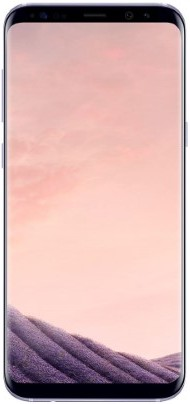
\includegraphics[width=5cm]{galaxy}};
% \end{tikzpicture}
%   \end{center}
% \end{frame}

% \begin{frame}{Machine Learning for Multiclass Prediction}
%   \[ {y} = g({x}; {\theta}) \]
% \end{frame}

\begin{frame}{Machine Learning for Multiclass Classification}


  \begin{center}
    \begin{tikzpicture}
      \node(a) [rectangle,  xshift=-5cm, scale=0.6, draw,thick,fill=blue!0, rounded corners, inner sep =5pt] {
        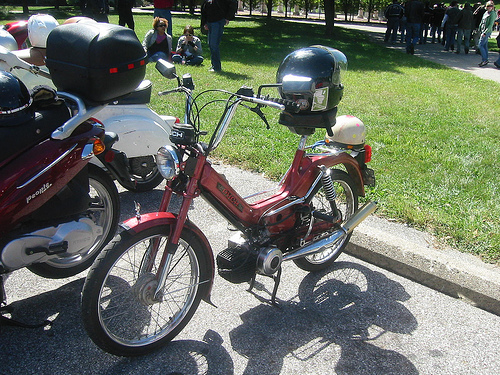
\includegraphics[width=7cm]{moped}};
      \node [rounded corners, above =(0.2cm) of a] {\alert<1>{$x$}};


      \visible<2->{
      \node(gal){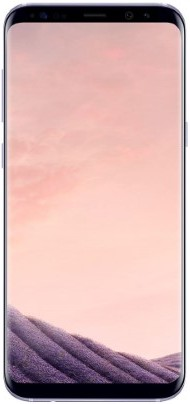
\includegraphics[width=1.5cm]{galaxy}};
      \node [rounded corners, above =(0.2cm) of gal] {\alert<2>{$g(\cdot; \alert<4>{\theta})$}};
\path[draw, ->] (a) --  (a -|  gal.west) ;
    }



\visible<3->{

  \node (b) [xshift=4.2cm, rectangle, draw,thick,fill=blue!0,text width=8em, rounded corners, inner sep =5pt, minimum height=1em, text centered]{\baselineskip=50pt  \centering Moped};
  \node [rounded corners, above = (0.2cm) of b] {\alert<3>{$y$}};
  \path[draw, <-] (b) --  (b -| gal.east);
  }

\end{tikzpicture}
\end{center}
\note{If you have seen any problem in machine learning, its probably multiclass prediction. Here we are given an input x, which is passed to a model g, to predict a label y. The model's parameters $\theta$ 
are set by looking at a large set of labeled examples. A major story in the last decade of machine learning has been the improvement of these types of tasks based on deep learning models. Deep learning 
here describes the form and structure of the model g and its parameters theta.   }
\end{frame}


\begin{frame}{Machine Learning for Text Generation}

  \[ \alert<3>{y^*_{1:T}} = \argmax_{y_{\tikzmark{opt}1:T}} \alert<4>{f}(\alert<3>{y_{1:T}}, \tikzmark{input}\alert<2>{x}; \tikzmark{nn}\alert<4>{\theta}) \]

% \begin{tikzpicture}[
%   remember picture,
%   overlay]

% \node (ptdex) [below left=  of {pic cs:pd}] {Output};
% \node (ptdexa) [below right =  of {pic cs:nn}] {Neural Network};
% \node (ptdexb) [below = of {pic cs:opt}] {Optimization};
% \node (ptdexc) [below = of {pic cs:input}] {Input};
% \draw[->] (ptdex.north) -- ({pic cs:pd});
% \draw[->] (ptdexa.north) -- ({pic cs:nn});
% \draw[->] (ptdexb.north) -- ({pic cs:opt});
% \draw[->] (ptdexc.north) -- ({pic cs:input});
% \end{tikzpicture}

  \begin{itemize}
    \pause
  \item Input \alert<2>{$x$},  \textit{what to talk about}
    \air
    \pause
  \item Output text \alert<3>{$y^*_{1:T}$}, \textit{how to say it}
    \air
    \pause
  \item Model \alert<4>{$f(.; \theta)$}, learned from data
  \end{itemize}
\end{frame}


\begin{frame}{Part 1: Generating Text}
  \begin{center}
    \begin{tikzpicture}
      \node[draw, fill=yellow, thick, rounded corners] (app) at (0mm,
      0mm) {Applications};
    \end{tikzpicture}
  \end{center}
\end{frame}


\begin{frame}{Machine Translation}
  \begin{center}
    \begin{tikzpicture}

      \node (gal) {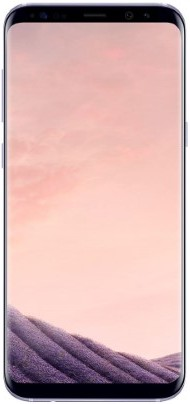
\includegraphics[width=1.5cm]{galaxy}};
      \node [rounded corners, above =(0.2cm) of gal] {$f$};

      \node (a) [rectangle, yshift=1cm, xshift=-5cm, scale=0.8, draw,thick,fill=blue!0,text width=16em, rounded corners, inner sep =5pt, minimum height=1em] {
        Yalitza Aparicio acababa de graduarse de una escuela para maestros y aun no tenia empleo cuando el proceso de busqueda de actrices para la ultima pelicula de Alfonso Cuaron llego a su natal Tlaxiaco, Oaxaca.
};
      \path[draw, ->] (a) --  (a -|  gal.west) ;


      \node [rounded corners, above =(0.2cm) of a] {\alert<1>{$x$}};

      \visible<2>{
        \node(b) [xshift=4.5cm, yshift=-1cm, rectangle, scale=0.8, draw,thick,fill=blue!0,text width=12em, rounded corners, inner sep =5pt, minimum height=1em]{\baselineskip=50pt \small
          Yalitza Aparicio had just finished her teaching degree and didn't yet have a job when the Mexican director Alfonso Cuaron held a casting call in her home of Tlaxiaco, Oaxaca, for the lead role in his semi-autobiographical drama, ``Roma.''
          \par};

        \node [rounded corners, above = (0.2cm) of b] {\alert<2>{$y^*_{1:T}$}};
        \path[draw, <-] (b) --  (b -| gal.east) ;
      }
    \end{tikzpicture}
  \end{center} 
\end{frame}


\begin{frame}{Translation Performance}
  

\textbf{Evaluation Metric:} 

Target:\  \
\texttt{[Yalitza Aparicio had] just [finished her] teaching [degree] .}
\air 

Predict:
\texttt{[Yalitza Aparicio had] recently [finished her] [degree]. }
\pause

\air 
\textbf{Deep Learning Performance:} 
  \begin{center}
     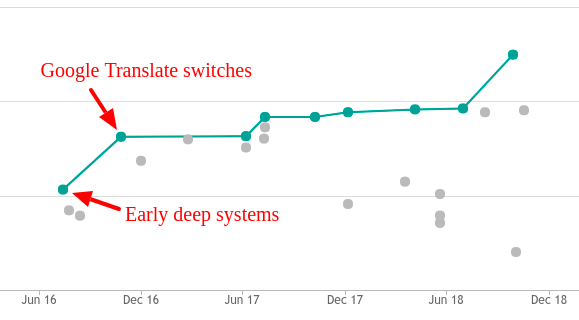
\includegraphics[width=8cm]{wmt}
  \end{center}
\end{frame}

\begin{frame}{Sentence Summarization }




  \begin{center}
    \begin{tikzpicture}

      \node (gal) {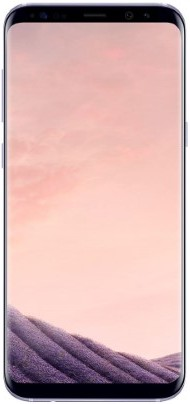
\includegraphics[width=1.5cm]{galaxy}};
      \node [rounded corners, above =(0.2cm) of gal] {$f$};


      \node (a) [rectangle, yshift=1cm, xshift=-5cm, scale=0.8, draw,thick,fill=blue!0,text width=20em, rounded corners, inner sep =5pt, minimum height=1em] {
        \small
        Cambodian leader Hun Sen on friday rejected opposition parties' demands for talks outside the country, accusing them of trying to ``internationalize'' the political crisis.};
      \path<2>[draw, ->] (a) --  (a -|  gal.west) ;


      \node [rounded corners, above =(0.2cm) of a] {\alert<1>{$x$}};

      \visible<2>{
        \node(b) [xshift=4.5cm, yshift=-1cm, rectangle, scale=0.8, draw,thick,fill=blue!0,text width=12em, rounded corners, inner sep =5pt, minimum height=1em]{\baselineskip=50pt \small
          Cambodian government rejects opposition's call for talks abroad
          \par};

        \node [rounded corners, above = (0.2cm) of b] {\alert<2>{$y_{1:T}$}};
        \path[draw, <-] (b) --  (b -| gal.east) ;
      }
    \end{tikzpicture}
  \end{center}
\end{frame}


\begin{frame}{GigaWord Dataset}
  \research{\citet{Rush2015} w/ Facebook}

  \begin{center}
    
\includegraphics[width=7cm]{ap}
  \end{center}
  \begin{itemize}
  \item Several million headlines paired with article leads.
  \item Simple model for  abstractive summarization / compression. 
  \item Benchmark dataset for early deep summarization work.
  \end{itemize}
\end{frame}



\begin{frame}{Sentence Summarization}

  \begin{center}
    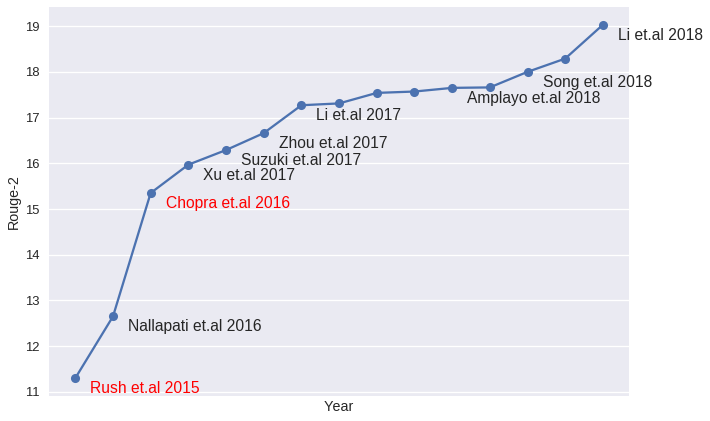
\includegraphics[height=0.75\textheight]{Gigaword}
  \end{center}

\end{frame}

\begin{frame}{Document Summary}
  \begin{center}
    \begin{tikzpicture}

      \node{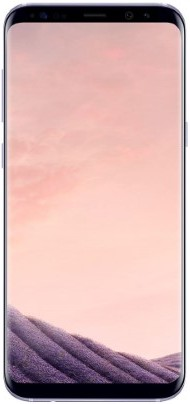
\includegraphics[width=1.5cm]{galaxy}};



      \node(a) [rectangle, yshift=0.2cm, xshift=-5cm, scale=0.6, draw,thick,fill=blue!0,text width=25em, rounded corners, inner sep =5pt, minimum height=1em] {
        \small
        London, England  (reuters) -- Harry Potter star Daniel Radcliffe gains access to a reported \$20 million fortune as he turns 18 on monday, but he insists the money won't  cast a spell on him. Daniel Radcliffe as harry potter in ``Harry Potter and the Order of the Phoenix'' to the disappointment of gossip columnists around the world , the young actor says he has no plans to fritter his cash away on fast cars , drink and celebrity parties . `` i do n't plan to be one of those people who , as soon as they turn 18 , suddenly buy themselves a massive sports car collection or something similar , '' he told an australian interviewer earlier this month . `` i do n't think i 'll be particularly extravagant '' . `` the things i like buying are things that cost about 10 pounds -- books and cds and dvds . '' at 18 , radcliffe will be able to gamble in a casino , buy a drink in a pub or see the horror film `` hostel : part ii , '' currently six places below his number one movie on the uk box office chart  . details of how he 'll mark his landmark birthday are under wraps . his agent and publicist had no comment on his plans . `` i 'll definitely have some sort of party , '' he said in an interview $\ldots$ %`` hopefully none of you will be reading about it . '' radcliffe 's earnings from the first five potter films have been held in a trust fund which he has not been able to touch . despite his growing fame and riches , the actor says he is keeping his feet firmly on the ground . `` people are always $\ldots$
};

\path[draw, ->] (a) --  (a -|  gal.west) ;

\visible<2>{
  \node (b) [xshift=4.2cm, yshift=-0.2cm, rectangle, scale=0.8, draw,thick,fill=blue!0,text width=12em, rounded corners, inner sep =5pt, minimum height=1em]{\baselineskip=50pt \footnotesize
    Harry Potter star Daniel Radcliffe gets \$20m fortune as he turns 18 monday. Young actor says he has no plans to fritter his cash away. Radcliffe 's earnings from first five potter films have been held in trust fund.  \par};
  \path[draw, <-] (b) --  (b -| gal.east);
  }

\end{tikzpicture}
\end{center}
\end{frame}


\begin{frame}{Document Summarization}
  \begin{center}
    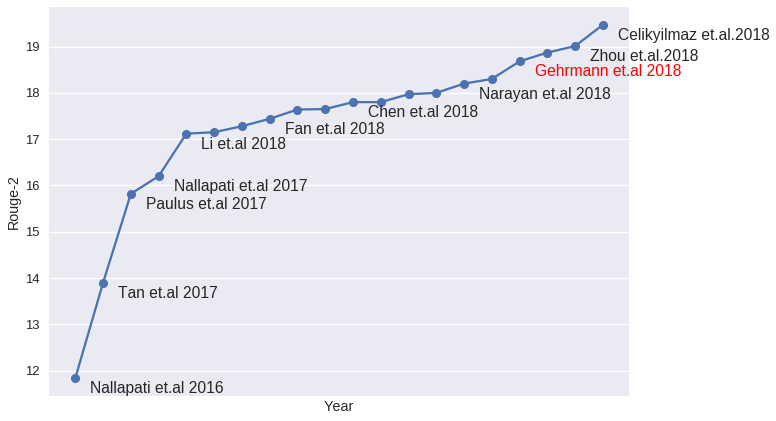
\includegraphics[height=0.75\textheight]{CNNDM}
  \end{center}
\end{frame}


\begin{frame}{Talk about Data }

  \research{\cite{EMNLP2017}}
  \begin{center}
\begin{tikzpicture}
\node[]{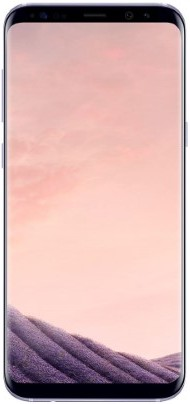
\includegraphics[width=1.5cm]{galaxy}};



\node(a)[xshift=-4.5cm, draw, scale=0.5, inner sep=10pt, rounded corners, text width=26em]{
\small
  \begin{center}

\begin{tabular}{lcccccc}
\toprule
{} & WIN & LOSS & PTS & FG\_PCT & RB & AS \ldots \\
TEAM &           &             &          &             &          &          \\
\midrule
Heat      &        11 &          12 &      103 &          49 &       47 &       27 \\
Hawks     &         7 &          15 &       95 &          43 &       33 &       20 \\
\bottomrule
\end{tabular}
\vspace{0.5cm}

\begin{tabular}{lccccccccc}
\toprule
{} &  AS &    RB &   PT &  FG &  FGA & CITY  $\ldots$ \\
PLAYER      &      &      &      &       &      &      &           \\
\midrule
Tyler Johnson    &    5 &    2 &  27 &    8 &   16 &     Miami \\
Dwight Howard    &    11 &    17 &  23 &    9 &   11 &   Atlanta \\
Paul Millsap     &    2 &    9 &  21 &    8 &   12 &   Atlanta \\
Goran Dragic     &    4 &    2 &  21 &    8 &   17 &     Miami \\
Wayne Ellington  &    2 &    3 &  19 &    7 &   15 &     Miami \\
Dennis Schroder  &    7 &    4 &  17 &    8 &   15 &   Atlanta \\
Rodney McGruder  &    5 &    5 &  11 &    3 &    8 &     Miami \\
\ldots \\
\bottomrule
\end{tabular}
  \end{center}
};

\path[draw, ->] (a) --  (a -|  gal.west) ;


% \node[inner sep=1pt, rounded corners, text width=15em, xshift=-4cm,]{\small
%   \begin{center}
% \vspace{0.5cm}
% \footnotesize
% \begin{tabular}{lcccccc}
% \toprule
% {} & W & L & PTS &  \ldots \\
% TEAM &           &             &          &                      \\
% \midrule
% Heat   &        11 &          12 &      103 &     \ldots      \\
% Hawks  &         7 &          15 &       95 &     \ldots      \\
% \bottomrule

% \vspace*{0.3cm}
% \end{tabular}

% % \begin{tabular}{lccccccccc}
% % \toprule
% % {} &  AS &    RB &   PT &  FG &  FGA & CITY  $\ldots$ \\
% % PLAYER      &      &      &      &       &      &      &           \\
% % \midrule
% % Tyler Johnson    &    5 &    2 &  27 &    8 &   16 &     Miami \\
% % Dwight Howard    &    11 &    17 &  23 &    9 &   11 &   Atlanta \\
% % Paul Millsap     &    2 &    9 &  21 &    8 &   12 &   Atlanta \\
% % Goran Dragic     &    4 &    2 &  21 &    8 &   17 &     Miami \\
% % Wayne Ellington  &    2 &    3 &  19 &    7 &   15 &     Miami \\
% % Dennis Schroder  &    7 &    4 &  17 &    8 &   15 &   Atlanta \\
% % Rodney McGruder  &    5 &    5 &  11 &    3 &    8 &     Miami \\
% % \ldots \\
% % \bottomrule
% % \end{tabular}

%   \end{center}




% };
 % \node [xshift=-3.5cm, rectangle, draw,thick,fill=blue!0,text width=8em, rounded corners, inner sep =5pt, minimum height=1em]{\baselineskip=50pt \footnotesize The Atlanta Hawks defeated the Miami Heat, 103 - 95, at Philips Arena on Wednesday. Atlanta  ... \par};
\visible<2>{\node(b) [xshift=4.5cm,scale=0.5,  rectangle, draw,thick,fill=blue!0,text width=26em, rounded corners, inner sep =10pt, minimum height=1em]{\baselineskip=100pt \large  The Atlanta Hawks defeated the Miami Heat, 103 - 95, at Philips Arena on Wednesday. Atlanta was in desperate need of a win and they were able to take care of a shorthanded Miami team here. Defense was key for the Hawks, as they held the Heat to 42 percent shooting and forced them to commit 16 turnovers. Atlanta also dominated in the paint, winning the rebounding battle, 47 - 34, and outscoring them in the paint 58 - 26. The Hawks shot 49 percent from the field and assisted on 27 of their 43 made baskets. This was a near wire-to-wire win for the Hawks, as Miami held just one lead in the first five minutes. Miami ( 7 - 15 ) are as beat-up as anyone right now and it's taking a toll on the heavily used starters. Hassan Whiteside really struggled in this game, as he amassed eight points, 12 rebounds and one blocks on 4 - of - 12 shooting ... \par};

  \path[draw, <-] (b) --  (b -| gal.east);
}
% \visible<2>{\node[xshift=3.5cm, rectangle, draw,thick,fill=blue!0,text width=8em, rounded corners, inner sep =5pt, minimum height=1em]{\baselineskip=50pt \footnotesize The Atlanta Hawks defeated the Miami Heat, 103 - 95, at Philips Arena on Wednesday. Atlanta  ... \par};}
\end{tikzpicture}
  \end{center}
\end{frame}


% \begin{frame}
%   \begin{center}
%     \textbf{Case Study: Data-to-Document Generation}
%   \end{center}

% \vspace{-0.7cm}
%   \begin{figure}
% \centering
% \scalebox{0.6}{
% \begin{tikzpicture}
% \node[draw, inner sep=10pt, rounded corners, text width=30em, xshift=-7.5cm,]{\small
%   \begin{center}


% \begin{tabular}{lcccccc}
% \toprule
% {} & WIN & LOSS & PTS & FG\_PCT & RB & AS \ldots \\
% TEAM &           &             &          &             &          &          \\
% \midrule
% Heat      &        11 &          12 &      103 &          49 &       47 &       27 \\
% Hawks     &         7 &          15 &       95 &          43 &       33 &       20 \\
% \bottomrule
% \end{tabular}
% \vspace{0.5cm}

% \begin{tabular}{lccccccccc}
% \toprule
% {} &  AS &    RB &   PT &  FG &  FGA & CITY  $\ldots$ \\
% PLAYER      &      &      &      &       &      &      &           \\
% \midrule
% Tyler Johnson    &    5 &    2 &  27 &    8 &   16 &     Miami \\
% Dwight Howard    &    11 &    17 &  23 &    9 &   11 &   Atlanta \\
% Paul Millsap     &    2 &    9 &  21 &    8 &   12 &   Atlanta \\
% Goran Dragic     &    4 &    2 &  21 &    8 &   17 &     Miami \\
% Wayne Ellington  &    2 &    3 &  19 &    7 &   15 &     Miami \\
% Dennis Schroder  &    7 &    4 &  17 &    8 &   15 &   Atlanta \\
% Rodney McGruder  &    5 &    5 &  11 &    3 &    8 &     Miami \\
% \ldots \\
% \bottomrule
% \end{tabular}

%   \end{center}

% };


% \node [yshift=-4cm, rectangle, draw,thick,fill=blue!0,text width=30em, rounded corners, inner sep =10pt, minimum height=1em]{\baselineskip=100pt \large  The Atlanta Hawks defeated the Miami Heat, 103 - 95, at Philips Arena on Wednesday. Atlanta was in desperate need of a win and they were able to take care of a shorthanded Miami team here. Defense was key for the Hawks, as they held the Heat to 42 percent shooting and forced them to commit 16 turnovers. Atlanta also dominated in the paint, winning the rebounding battle, 47 - 34, and outscoring them in the paint 58 - 26. The Hawks shot 49 percent from the field and assisted on 27 of their 43 made baskets. This was a near wire-to-wire win for the Hawks, as Miami held just one lead in the first five minutes. Miami ( 7 - 15 ) are as beat-up as anyone right now and it's taking a toll on the heavily used starters. Hassan Whiteside really struggled in this game, as he amassed eight points, 12 rebounds and one blocks on 4 - of - 12 shooting ... \par};
% \end{tikzpicture}
% }
% \caption{\small Document generation example. Left, a source consisting of structured data, in this case statistics from a basketball game. Right, a target document utilizing a select subset of records from the data,
%   expressed in an often complex and expressive manner. This example is an excerpt from the case-study data set, which include
%   628 records in total and a longer target document. }
% \label{fig:samplesummary}
% \end{figure}

% \end{frame}


\begin{myverbbox}{\sTWO}
 { \cal K } ^ { L } ( \sigma = 2 ) = \left( \begin{array}
{ c c } { - \frac { d ^ { 2 } } { d x ^ { 2 } } + 4 - \frac
 { 3 } { \operatorname { c o s h } ^ { 2 } x } } \& { \frac
 { 3 } { d x ^ { 2 } } }  { \frac { 3 } { \operatorname
 { c o s h } ^ { 2 } x } } \& { - \frac { d ^ { 2 } }
{ d x ^ { 2 } } + 4 - \frac { 3 } { \operatorname { c o s h }
^ { 2 } x } }  \end{array} \right) \qquad
\end{myverbbox}

\begin{frame}{E2E Challenge 2018}
  \begin{figure}
    \centering

    \footnotesize
\begin{tabular}{@{}ll@{}}
\toprule
\bf MR        & \begin{tabular}[c]{@{}l@{}}name{[}The Golden Palace{]},  eatType{[}coffee shop{]},  food{[}Fast food{]}, \\ priceRange{[}cheap{]},  customer rating{[}5 out of 5{]},  area{[}riverside{]}\end{tabular}         \\ \midrule
\bf Reference & \begin{tabular}[c]{@{}l@{}}A coffee shop located on the riverside  called The Golden Palace,  \\ has a 5 out of 5 customer rating.  Its price range are fairly cheap  \\for its excellent Fast food.\end{tabular} \\ \bottomrule
\end{tabular}
  \end{figure}
  \begin{center}
    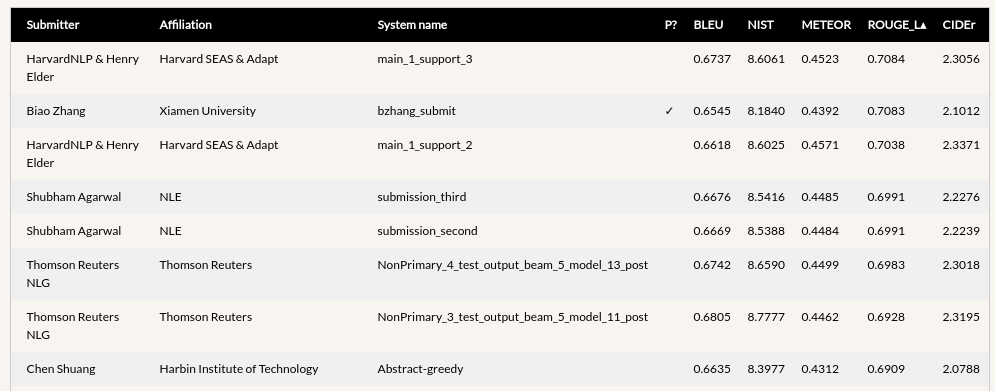
\includegraphics[width=\textwidth]{E2EChallenge}
  \end{center}
\end{frame}



\begin{frame}{Talk about the Diagrams}
\research{\cite{Deng2016} w/ Bloomberg}
  \begin{center}
\begin{tikzpicture}


\node(a){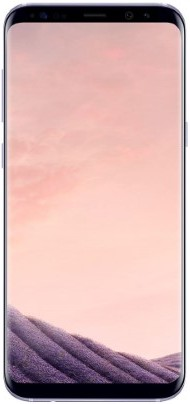
\includegraphics[width=1.5cm]{galaxy}};
 \node [yshift=4cm, rectangle, thick,fill=blue!0,text width=5cm, rounded corners, inner sep =5pt, minimum height=1em]{\baselineskip=50pt 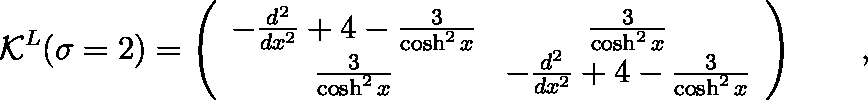
\includegraphics[width=10cm]{latexin}};

\visible<2> {
\node (b)[xshift=6cm, rectangle, scale=0.6, draw,thick,fill=blue!0,text width=32em, rounded corners, inner sep =5pt, minimum height=1em]{\baselineskip=50pt \footnotesize
\sTWO

};
  \path[draw, <-] (b) --  (b -| gal.east);
}
\end{tikzpicture}
  \end{center}
\end{frame}

\begin{frame}{Im2Latex}
\research{\cite{Deng2016} w/ Bloomberg}
\begin{center}
  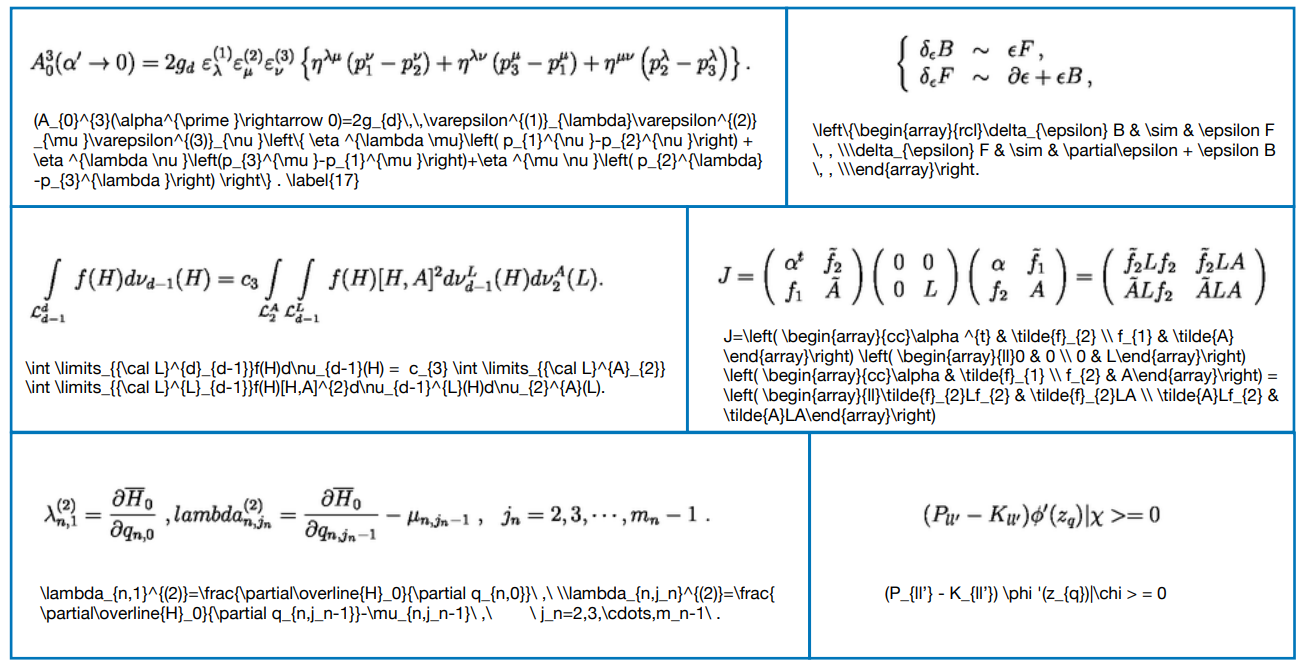
\includegraphics[height =0.75\textheight]{imlatex}
\end{center}
\end{frame}


\begin{frame}{Im2Latex}
\research{\cite{Deng2016} w/ Bloomberg}


  \vspace{-0.25cm}
  \begin{center}
    \movie[width=\textwidth, repeat, height=0.85\textheight, width=\textwidth, poster, showcontrols]{Temporary}{videos/latex.mp4}
  \end{center}

\end{frame}

% \section{Introduction}


% \begin{frame}

%   % Application pictures
% \end{frame}

% \begin{frame}{Text Generation}

%   \[ \argmax_{y_{1:T}} f(y_{1:T} ; x, \theta)\]

% \end{frame}

\begin{frame}
  NLP
\end{frame}

\begin{frame}{State-of-the-Art Natural Language Processing, circa 2009}

  % Picture
  \begin{center}

    \scalebox{0.8}{
  \begin{tikzpicture}[node distance=0.2cm]
    \node(task)[minimum height=2em] {\textbf{Task}};
    \node(aa) [draw, rounded corners, minimum width=12em,minimum height=3em, below= of task]{Syntax};
    \node(bb) [draw, rounded corners, minimum width=12em,minimum height=3em, below= of aa]{Surface Structure};
    \node(cc) [draw, rounded corners, minimum width=12em,minimum height=3em, below= of bb]{Translation};
    \node(dd) [draw, rounded corners, minimum width=12em,minimum height=3em, below= of cc]{Summarization};
    \node(ee) [draw, rounded corners, minimum width=12em,minimum height=3em, below= of dd]{Coreference};
    \node     [below= of ee]{$\vdots$};


    \visible<2>{
    \node(model) [minimum height=2em, right= of task, xshift=5cm]{\textbf{Model Class}};
    \node(a) [draw, rounded corners, minimum width=10em, minimum height=3em, below= of model]{Parsing};
    \node(b) [draw, rounded corners, minimum width=10em, minimum height=3em, below= of a]{CRF Tagging};
    \node(c) [draw, rounded corners, minimum width=10em, minimum height=3em, below= of b]{Alignment EM};
    \node(d) [draw, rounded corners, minimum width=10em, minimum height=3em, below= of c]{Logistic Regression};
    \node(e) [draw, rounded corners, minimum width=10em, minimum height=3em, below= of d]{Language Modeling};
    \node [below= of e]{$\vdots$};

    \draw (aa.east) -- (a.west);
    \draw (aa.east) -- (b.west);
    \draw (bb.east) -- (b.west);
    \draw (bb.east) -- (e.west);
    \draw (cc.east) -- (c.west);
    \draw (cc.east) -- (e.west);
    \draw (dd.east) -- (a.west);
    \draw (dd.east) -- (c.west);
    \draw (dd.east) -- (e.west);
    \draw (ee.east) -- (a.west);
    \draw (ee.east) -- (b.west);
    \draw (ee.east) -- (c.west);
}
  \end{tikzpicture}
}
  \end{center}
\end{frame}

\begin{frame}{State-of-the-Art Natural Language Processing, circa 2019}
\begin{center}
    \scalebox{0.8}{
  \begin{tikzpicture}[node distance=0.2cm]
    \node(task)[minimum height=2em] {\textbf{Task}};
    \node(aa) [draw, rounded corners, minimum width=12em,minimum height=3em, below= of task]{Syntax};
    \node(bb) [draw, rounded corners, minimum width=12em,minimum height=3em, below= of aa]{Surface Structure};
    \node(cc) [draw, rounded corners, minimum width=12em,minimum height=3em, below= of bb]{Translation};
    \node(dd) [draw, rounded corners, minimum width=12em,minimum height=3em, below= of cc]{Summarization};
    \node(ee) [draw, fill=red!10, rounded corners, minimum width=12em,minimum height=3em, below= of dd]{New Tasks};
    \node     [below= of ee]{$\vdots$};


   \visible<2>{
    \node(model) [minimum height=2em, right= of task, xshift=5cm]{\textbf{Model Class}};
    \node(a) [draw, rounded corners, minimum width=10em, minimum height=3em, below= of model, yshift=-2.5cm]{Neural Networks};

    \node[below=of a]{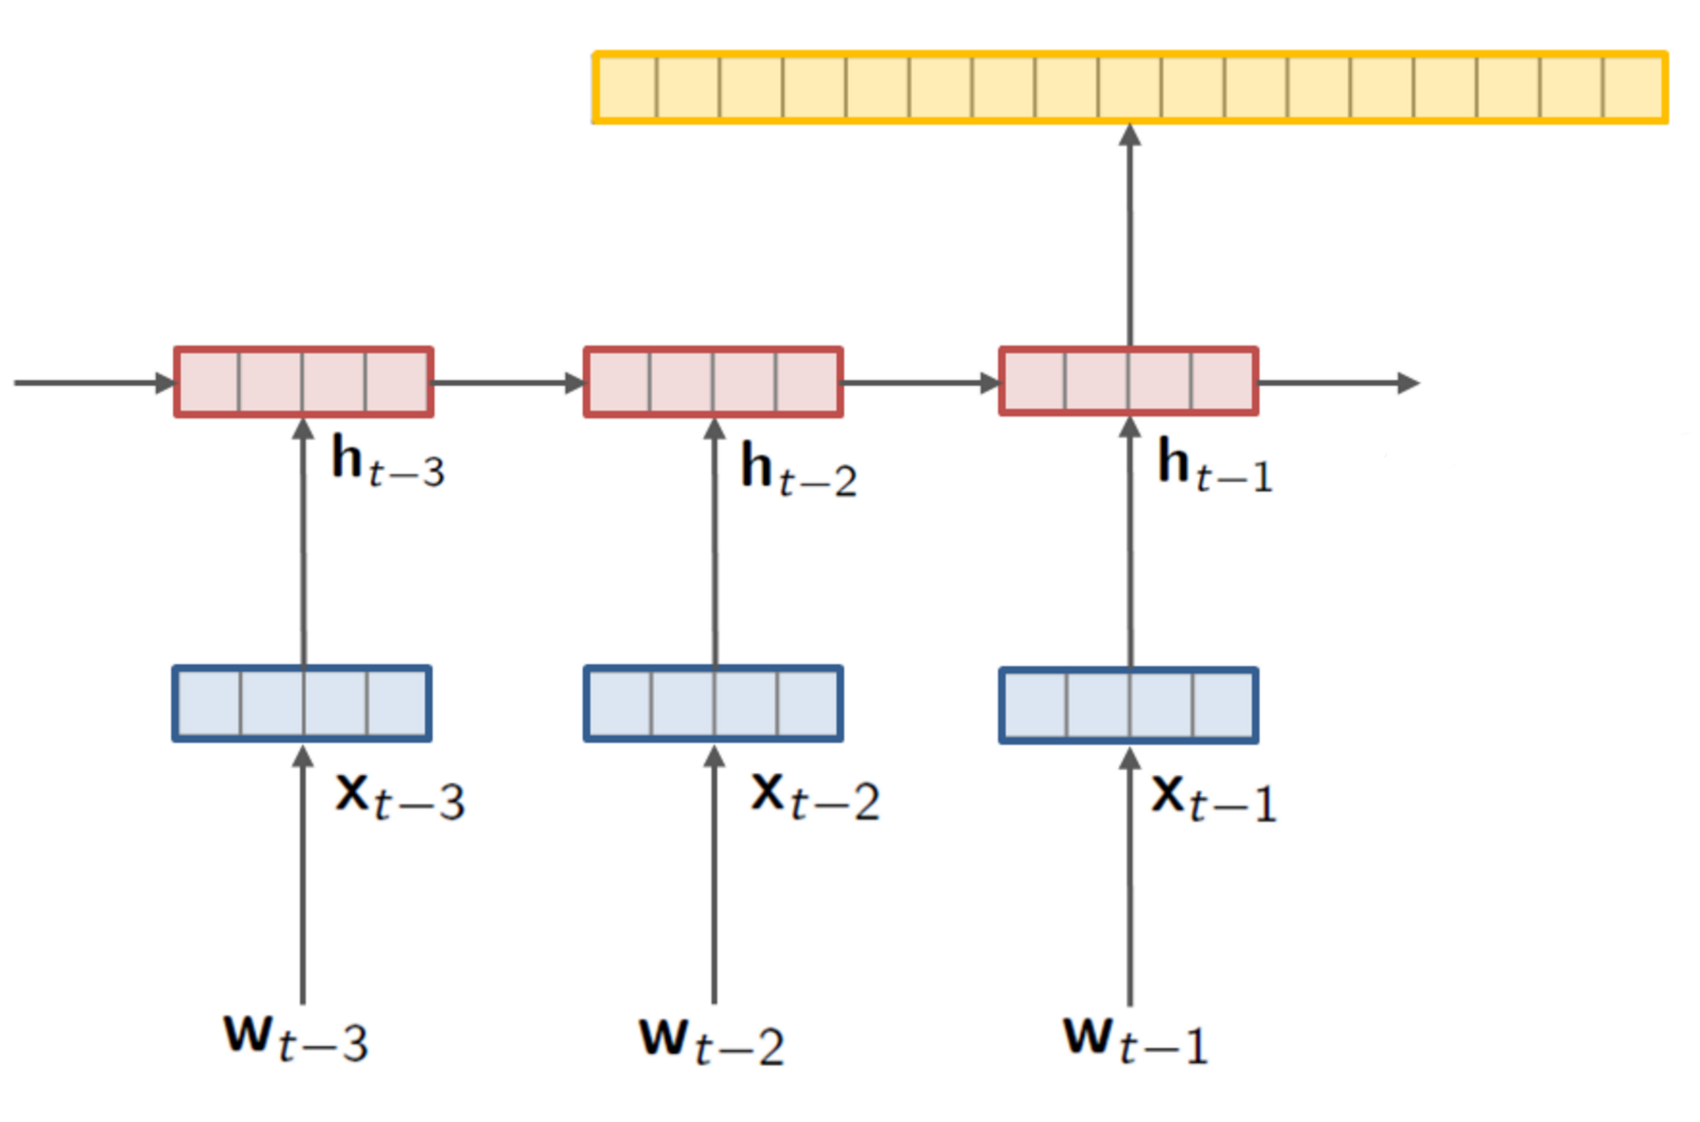
\includegraphics[width=4cm]{rnnlm6}};

    % \node[below  = of a, xshift=3cm]{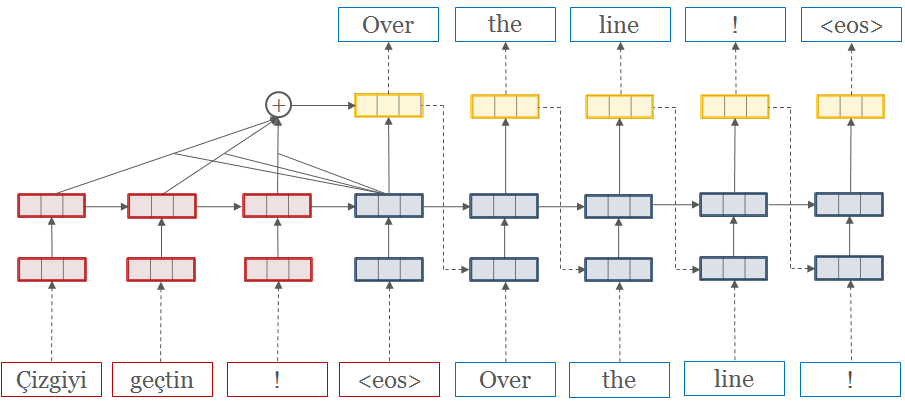
\includegraphics[width=8cm]{nmt}} ;

    % \node(b) [draw, rounded corners, minimum width=10em, minimum height=3em, below= of a]{CRF Tagging};
    % \node(c) [draw, rounded corners, minimum width=10em, minimum height=3em, below= of b]{Alignment EM};
    % \node(d) [draw, rounded corners, minimum width=10em, minimum height=3em, below= of c]{Logistic Regression};
    % \node(e) [draw, rounded corners, minimum width=10em, minimum height=3em, below= of d]{Language Modeling};
    \node [below= of e]{$\vdots$};

    \draw (aa.east) -- (a.west);
    \draw (bb.east) -- (a.west);
    \draw (cc.east) -- (a.west);
    \draw (dd.east) -- (a.west);
    \draw (ee.east) -- (a.west);
}

  \end{tikzpicture}
}


\end{center}
\end{frame}

% \begin{frame}{Performance}

% \end{frame}


% \begin{frame}

% \end{frame}

% \begin{frame}{Central}
%   % Picture
%   \begin{tikzpicture}
%     \node{};
%   \end{tikzpicture}
% \end{frame}


\begin{frame}{Harvard NLP Deep Learning Research}{}
  % Picture
  % \research{\cite{Deng2016}}

  \begin{center}
    \scalebox{2}{
  \begin{tikzpicture}

    \node<1> at (10mm, 15mm){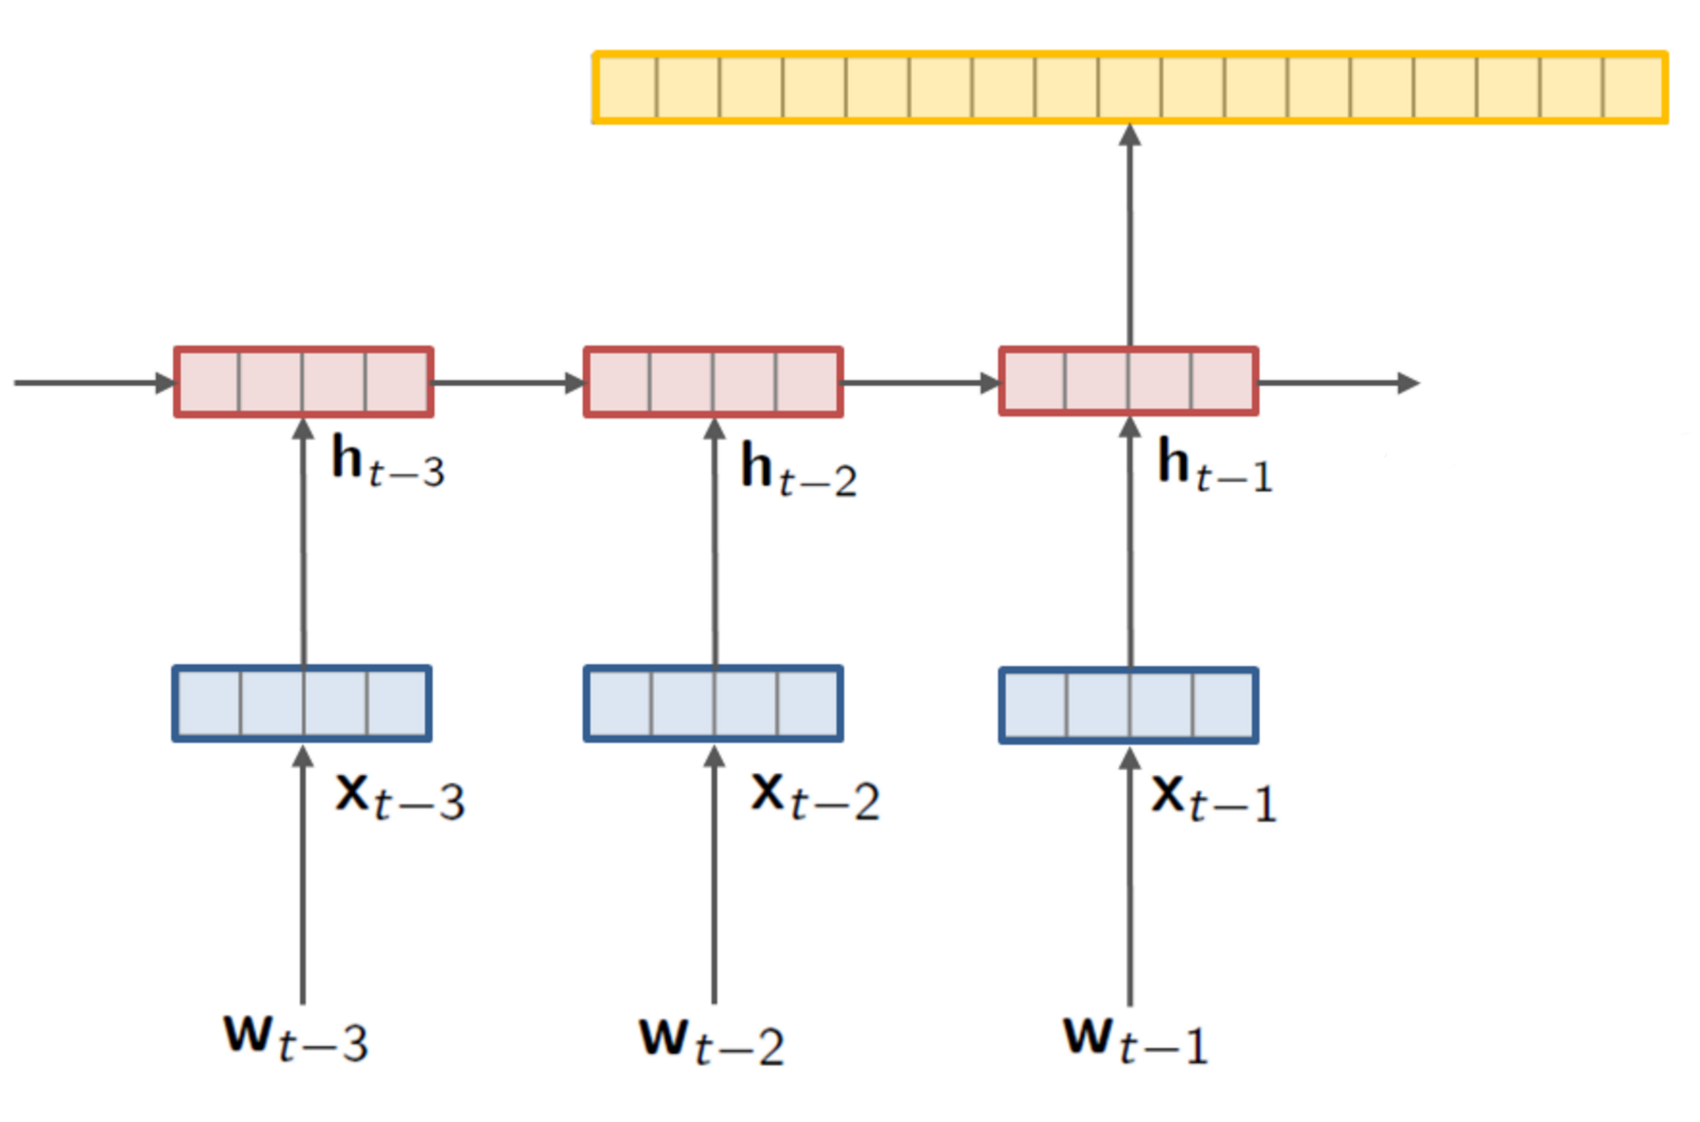
\includegraphics[width=3cm]{rnnlm6}};

    \node[draw,  thick, rounded corners, scale=0.5] (ana) at (-15mm, 15mm) {Analysis};
    \node[draw,  thick, rounded corners,scale=0.5] (meth) at (0mm, 30mm) {\ Methods\phantom{p}};
    \node[draw,  thick, rounded corners,scale=0.5] (app) at (25mm, 30mm) {Applications};
    \node<2>[draw,  fill=yellow, thick, rounded corners,scale=0.5] (app) at (25mm, 30mm) {Applications};
    \node<2>[scale=0.5, text width=35mm] at (10mm, 15mm) {\small \centering Translation, \\  Summary,  \\ Data-to-Text,  \\ Diagram-to-Text,  \\ $\vdots$};

    \node[draw, thick, rounded corners, scale=0.5] (und) at (35mm, 15mm) {Understanding};
    \node[draw, thick, rounded corners, scale=0.5] (dep) at (25mm, 0mm){Deployment};

    \node[draw,  thick, rounded corners,scale=0.5] (imp) at (0, 0) {Implementation};

    \draw (ana) -- (meth) --(app) -- (und) -- (dep) -- (imp) -- (ana);

  \end{tikzpicture}
}
  \end{center}

\end{frame}


\begin{frame}{Selected Harvard NLP Deep Learning Research}{}
  % Pictured

  \vspace{-1cm}

  \begin{center}
  \begin{tikzpicture}

    \node at (10mm, 15mm) {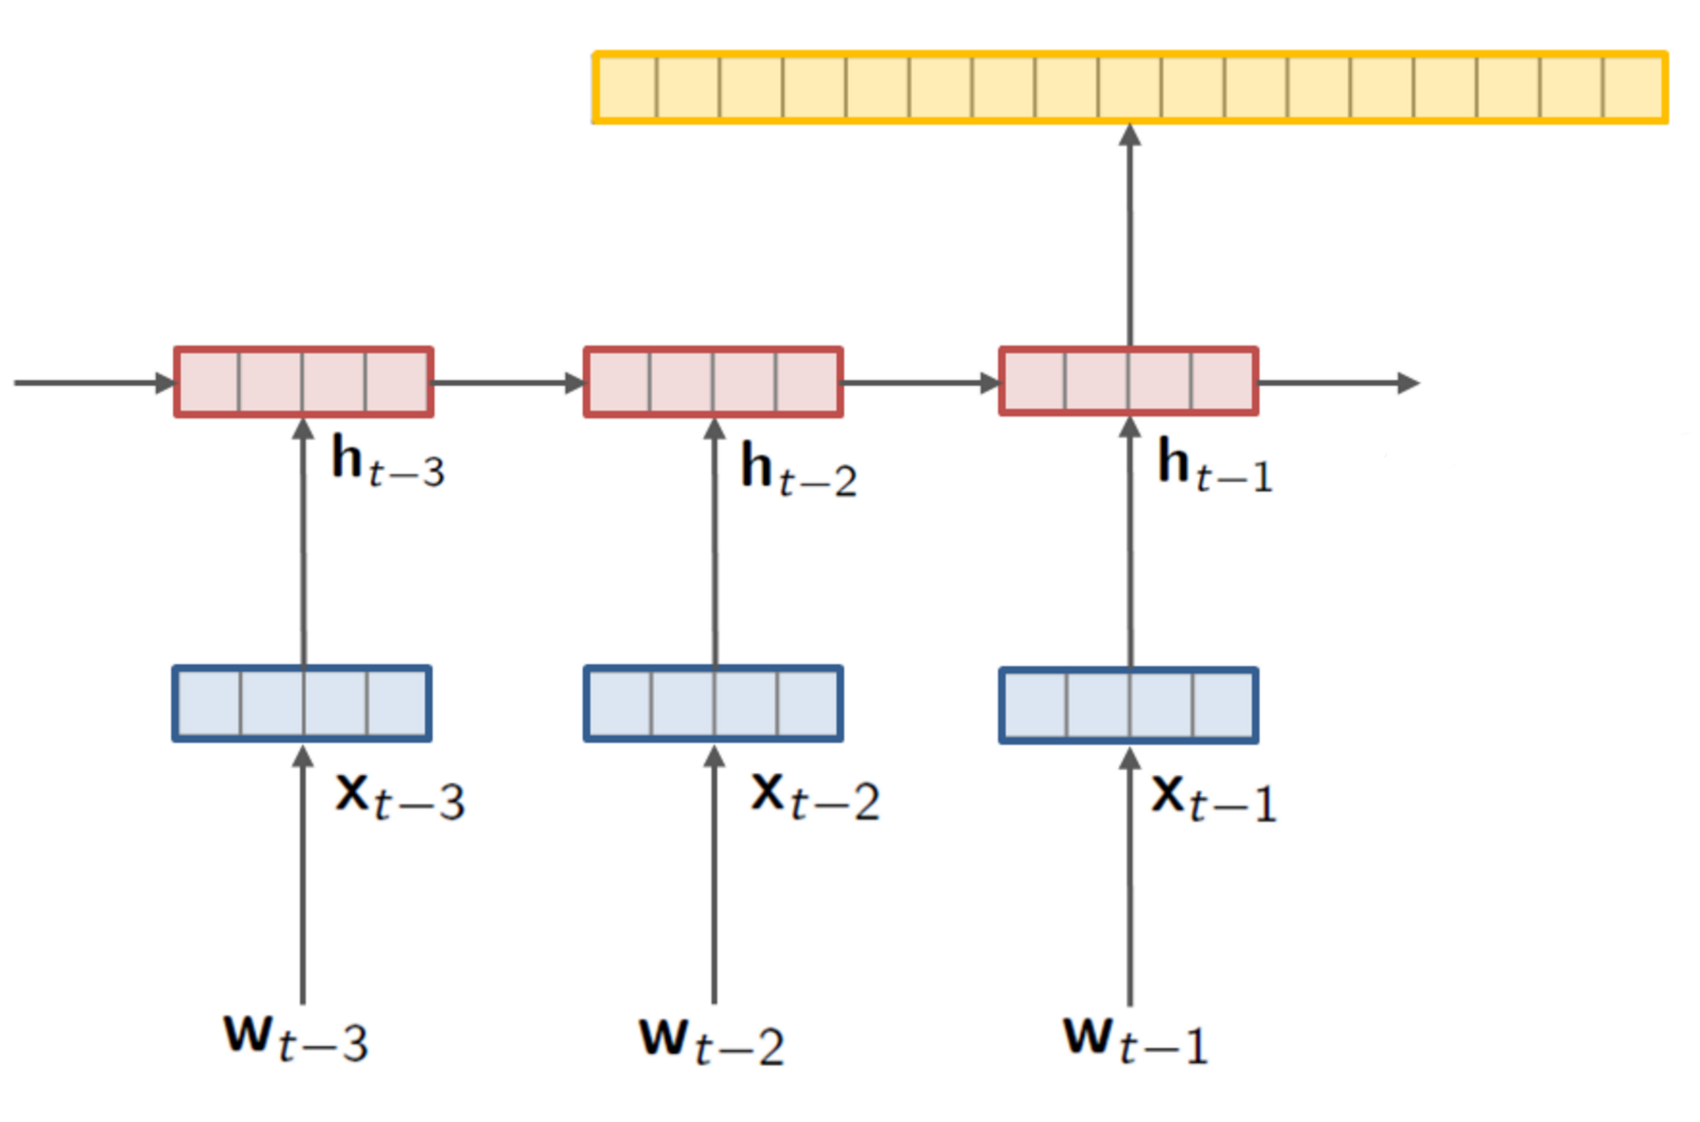
\includegraphics[width=2cm]{rnnlm6}};


    \node[rounded corners, draw] (ana) at (-15mm, 15mm) {Analysis};

    \visible<2,8>{
    \node at (-40mm, 15mm) [text width=30mm]{ \centering
      \baselineskip=-5pt  \scriptsize
      \structure{
      \citet{Strobelt2016}}
    \structure{
      \citet{strobelt2019s}}
      \citet{DBLP:conf/emnlp/WisemanSR17}
      \par
      };
    }

    \node[rounded corners, draw] (meth) at (0mm, 30mm) {\ Methods\phantom{p}};

    \visible<3,8>{
    \node at (-10mm, 35mm) [anchor=south, text width=30mm] { \centering

      \baselineskip=-5pt \scriptsize
      \citet{Kim2016} \ \
      \textcolor{red}{\cite{DBLP:journals/corr/KimDHR17}}\ \
      \cite{EMNLP2017}
      \par
      };
    }
    \node[rounded corners, draw] (app) at (25mm, 30mm) {Applications};

\visible<4,8>{

    \node at (35mm, 35mm) [anchor=south, text width=30mm]{ \centering
      \baselineskip=-5pt \scriptsize
      \citet{Rush2015}
      \textcolor{red}{\citet{Deng2016}}
      \citet{Schmaltz2016}
      \par
      };
}

    \node[rounded corners, draw] (und) at (35mm, 15mm) {Understanding};

\visible<5,8>{
    \node at (65mm, 15mm) [text width=30mm]{ \centering
      \baselineskip=-5pt \scriptsize
      \citet{wiseman2018learning}
      \textcolor{red}{\citet{deng2018latent}}\ \ \
      \textcolor{red}{\citet{DBLP:journals/corr/abs-1802-02550}}
      \par
      };
}

    \node[rounded corners, draw] (dep) at (25mm, 0mm){Deployment};

\visible<6,8>{
    \node at (35mm, -10mm) [text width=30mm] { \centering
            \baselineskip=-5pt \scriptsize
            \citet{Kim2016a}
            \citet{senellart2018opennmt}
            \alert{\citet{reagen2017weightless}}
            \par
      };
}
    \node at (75mm, -5mm) [draw, text width=35mm] {\centering
            \baselineskip=-5pt \scriptsize
            Natural Lang. Processing \\
            \alert{Machine Learning} \\
            \structure{Visualization}
            \par
      };


    \node[rounded corners, draw] (imp) at (0, 0) {Implement};
\visible<7,8>{
      \node at (-10mm, -10mm) [text width=30mm]{
        \baselineskip=-5pt \scriptsize
        \citet{DBLP:conf/acl/KleinKDSR17} \ \
        \citet{senellart2018opennmt} \ \
        \citet{rush2018annotated}
        \par
      };
}

    \draw (ana) -- (meth) --(app) -- (und) -- (dep) -- (imp) -- (ana);

  \end{tikzpicture}
  \end{center}
\end{frame}

% %%% Local Variables:
%%% TeX-master: "slides"
%%% End:

\section{Section 1}


\begin{frame}
  \begin{center}
    \scalebox{2}{
  \begin{tikzpicture}

    \node<1> at (10mm, 15mm){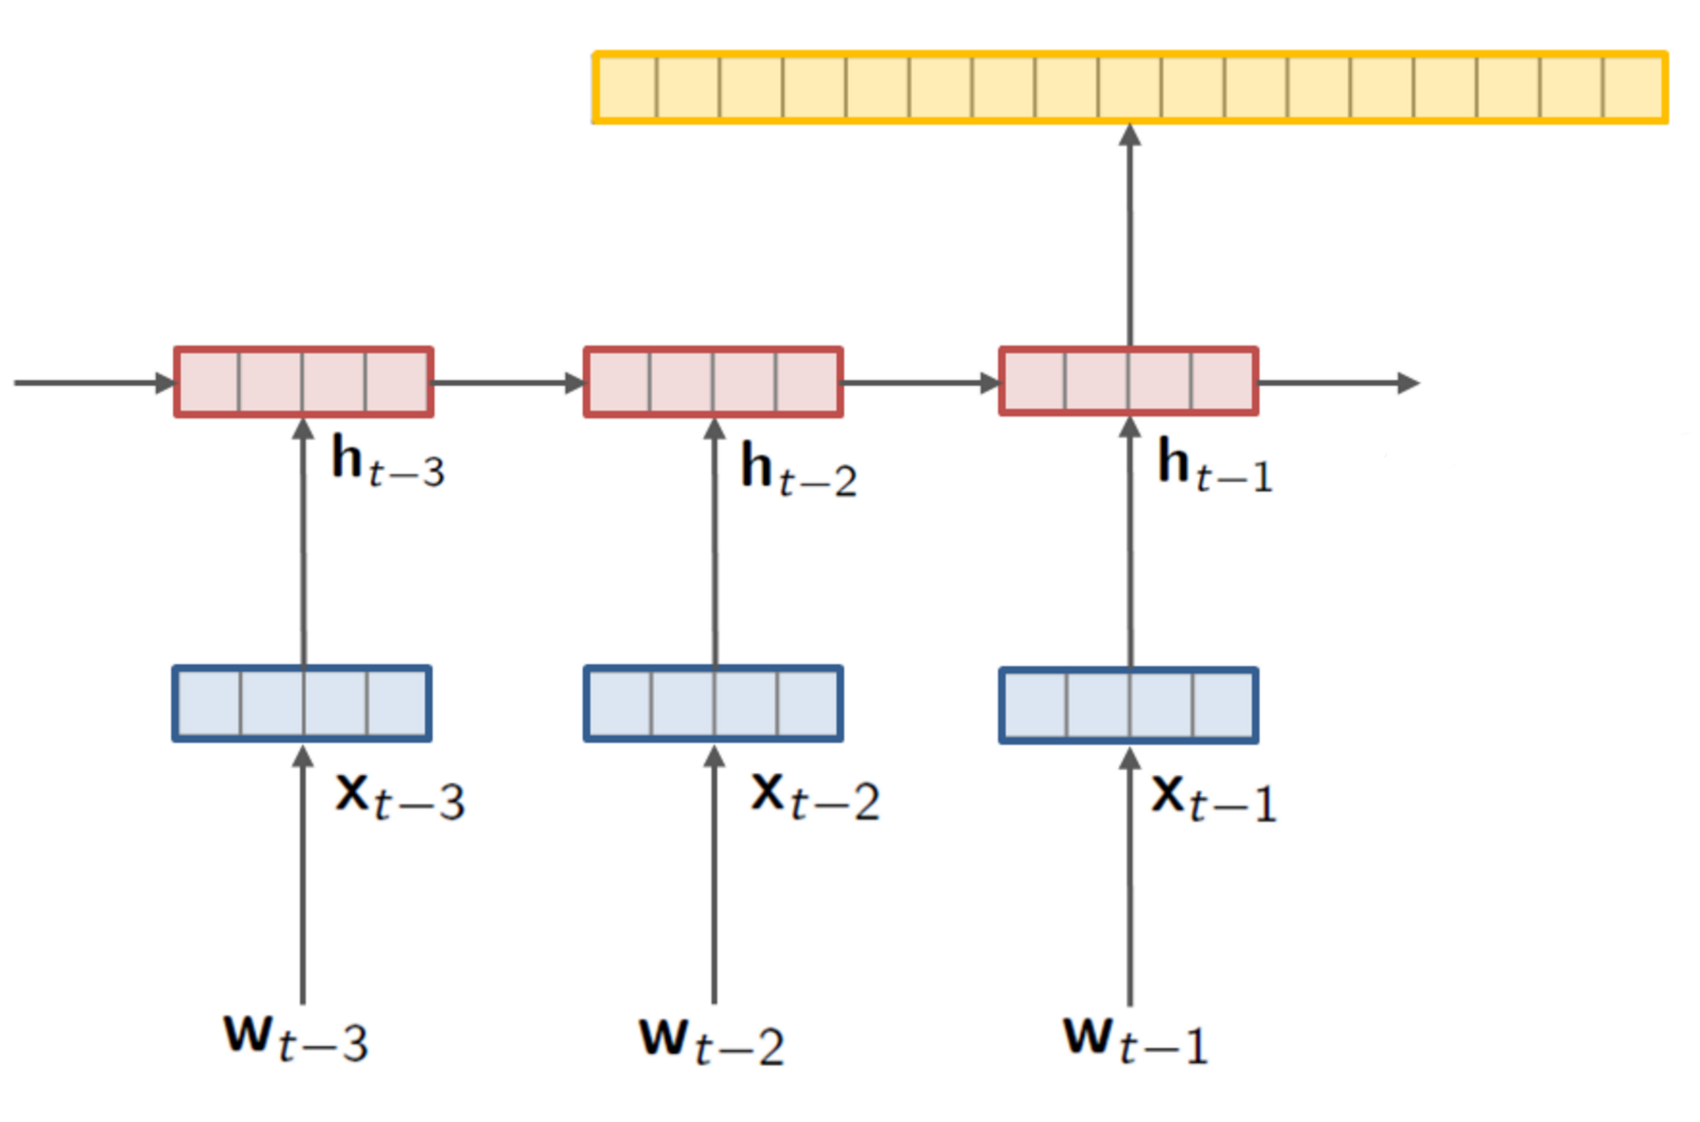
\includegraphics[width=3cm]{rnnlm6}};
    \node[draw,  fill=yellow, thick, rounded corners, scale=0.5] (ana) at (-15mm, 15mm) {Analysis};
    \node[draw,  thick, rounded corners,scale=0.5] (meth) at (0mm, 30mm) {\ Methods\phantom{p}};
    \node[draw,  thick, rounded corners,scale=0.5] (app) at (25mm, 30mm) {Applications};
    \node[draw, thick, rounded corners, scale=0.5] (und) at (35mm, 15mm) {Understanding};
    \node[draw, thick, rounded corners, scale=0.5] (dep) at (25mm, 0mm){Deployment};

    \node[draw, fill=yellow, thick, rounded corners,scale=0.5] (imp) at (0, 0) {Implementation};

    \draw (ana) -- (meth) --(app) -- (und) -- (dep) -- (imp) -- (ana);

  \end{tikzpicture}
}
  \end{center}


\end{frame}

\begin{frame}{Generation Setup (Reminder)}
    \[ \alert<3>{y^*_{1:T}} = \argmax_{y_{\tikzmark{opt}1:T}} \alert<4>{f}(\alert<3>{y_{1:T}}; \tikzmark{input}\alert<2>{x}, \tikzmark{nn}\alert<4>{\theta}) \] 

% \begin{tikzpicture}[
%   remember picture,
%   overlay]

% \node (ptdex) [below left=  of {pic cs:pd}] {Output};
% \node (ptdexa) [below right =  of {pic cs:nn}] {Neural Network};
% \node (ptdexb) [below = of {pic cs:opt}] {Optimization};
% \node (ptdexc) [below = of {pic cs:input}] {Input};
% \draw[->] (ptdex.north) -- ({pic cs:pd}); 
% \draw[->] (ptdexa.north) -- ({pic cs:nn}); 
% \draw[->] (ptdexb.north) -- ({pic cs:opt}); 
% \draw[->] (ptdexc.north) -- ({pic cs:input}); 
% \end{tikzpicture}

  \begin{itemize}
    \pause
  \item Input \alert<2>{$x_{1:S}$},  \textit{what to talk about}
    \air 

  \item Output text \alert<3>{$y^*_{1:T}$}, \textit{how to say it}
    \air

  \item Model \alert<4>{$f(.; \theta)$}, learned from data
  \end{itemize}
\end{frame}

\begin{frame}{Recurrent Neural Networks}
  \vspace{-0.25cm}

  \begin{center}
    \multiinclude[format=png,start=1,graphics={height=0.85\textheight}]{nmt-noattn}
  \end{center}
\end{frame}


\begin{frame}{RNN Math}
  \textcolor{blue}{Encoder}:
  \[{\mathbf{h}^{x}_s \gets \RNN(\mathbf{h}^{x}_{s-1}, x_s)} \]

  \textcolor{orange}{Context}:
  \[ {\mathbf{c}} = \mathbf{h}^{x}_S \]

  \textcolor{red}{Decoder}:
  \[{\mathbf{h}_t \gets \RNN(\mathbf{h}_{t-1}, y_t)} \]

  Prediction:
  \[ p(y_{t+1}\  |\  y_{1:t}, x) = \softmax( \mathbf{W} [\mathbf{h}_t, \mathbf{c}]) \]

  \pause 

  Generation:
  \[ \argmax_{y_{1:T}} f(y_{1:T}; x, \theta) = \argmax_{y_{1:T}} \prod_{t=1}^T p(y_{t+1}\  |\  y_{1:t}, x) \] 

\end{frame}

\begin{frame}{Toy Example: Parenthesis Language}
  \begin{center}
    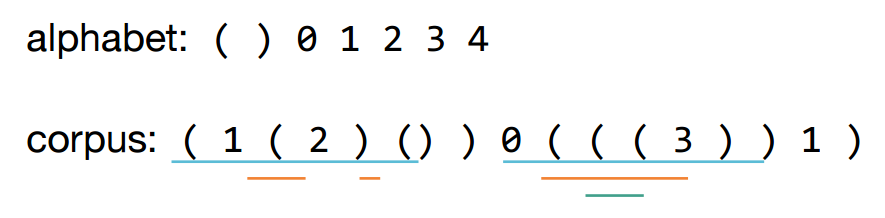
\includegraphics[width=10cm]{parenlang}
  \end{center}
\end{frame}

\begin{frame}{LSTMVis - Parenthesis Language}
  \research{\citet{Strobelt2016} w/ IBM}
  \vspace{-0.25cm}

  \begin{center}
    \movie[width=\textwidth, height=0.85\textheight, poster, showcontrols]{Temporary}{videos/lstmvis1.mp4}
  \end{center}
\end{frame}


\begin{frame}{LSTMVis - Natural Language}
  \research{\citet{Strobelt2016} w/ IBM}
  \vspace{-0.25cm}


  \begin{center}
    \movie[width=\textwidth, height=0.85\textheight, poster, showcontrols]{Temporary}{videos/lstmvis2.mp4}
  \end{center}
\end{frame}


\begin{frame}{Seq2Seq + Attention Model}
  \vspace{-0.25cm}

  \begin{center}
    \multiinclude[format=png,start=1,end=10,graphics={height=0.85\textheight}]{figs/nmt-attn}
  \end{center}
\end{frame}

\begin{frame}{Attention Math}

  \textcolor{blue}{Encoder}:
  \[{\mathbf{h}^{x}_s \gets \RNN(\mathbf{h}^{x}_{s-1}, x_s)} \]


  \textcolor{orange}{Attention}
  \[\alpha \gets  \softmax(   [\mathbf{h}^{x}_1 ; \ldots; \mathbf{h}^{x}_S]^\top \mathbf{h}_{t} ) \ \ \ \ 
  {\mathbf{c}} \gets \sum_{s =1}^S \alpha_s \mathbf{h}_s^{x}  \]

  \textcolor{red}{Decoder}:
  \[{\mathbf{h}_t \gets \RNN(\mathbf{h}_{t-1}, y_t)} \]

  Prediction:
  \[ p(y_{t+1}\  |\  y_{1:t}, x) = \softmax( \mathbf{W} [\mathbf{h}_t; \mathbf{c}]) \]

\end{frame}

\begin{frame}{Seq2SeqVis}
  \research{\citet{strobelt2019s} w/ IBM}
  \vspace{-0.25cm}

  \begin{center}
    \movie[width=\textwidth, height=0.85\textheight, poster, showcontrols]{Temporary}{videos/seq2seq.mp4}
  \end{center}
  
\end{frame}


\begin{frame}
  
  \begin{center}
    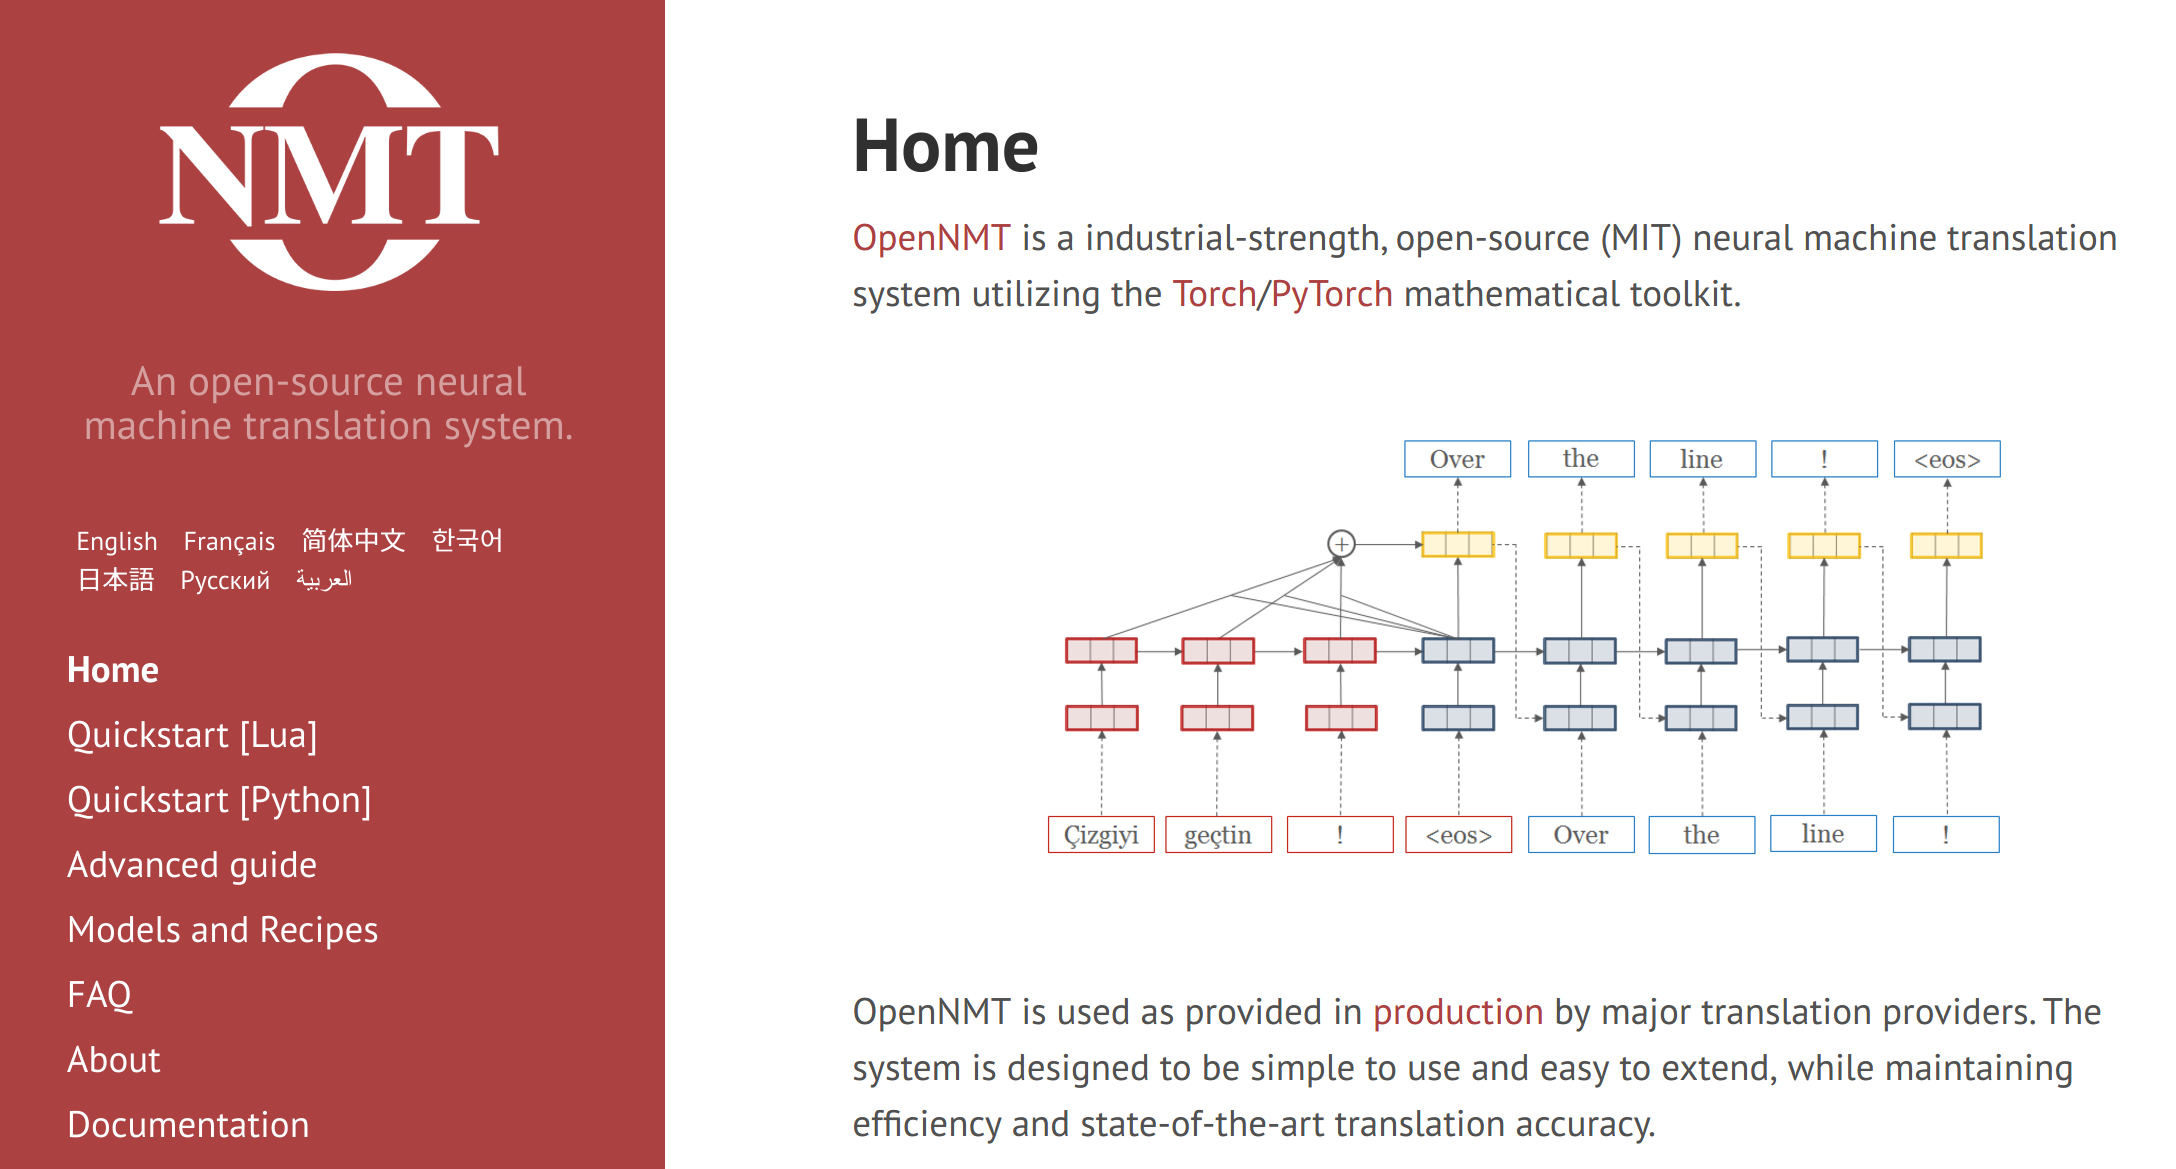
\includegraphics[width=\linewidth]{opennmt}
  \end{center}

\end{frame}

\begin{frame}
  \begin{center}
    
\includegraphics[width=3cm]{OpenNMT}
  \end{center}

  \begin{itemize}
  \item Collaborative open-source project started at Harvard, now self-sustaining.
    \air 
  \item Used in production by Systran, Ubiqus, Booking.com, and others.
    \air
  \item Over 100 developers in France, China, Japan, Portugal, and the US.
    \air
  \item Designed to be research extensible to latest machine translation techniques. 
    \air

  \item Pretrained models for translation as well as everything in this talk.
  \end{itemize}
\end{frame}

\begin{frame}
  \begin{center}
    \hspace*{-9cm}\includegraphics[height=0.5\textheight]{opennmtpanaram.jpg}
  \end{center}
\end{frame}

% \begin{frame}{Talk Outline}

  \begin{enumerate}
  \item Background: Core Model and Implementation
    \air
  \item \textbf{Work 1}: Rethinking Model Training (\textit{Beam Search Optimization})
    \air

  \item Work 2: Rethinking  Generation  (\textit{Learning Neural Templates})
    \air

  \item Future Directions
  \end{enumerate}
\end{frame}


% \begin{frame}{Part 3: Structured Modeling}
%   \begin{center}
%     \scalebox{2}{
%   \begin{tikzpicture}

%     \node<1> at (10mm, 15mm){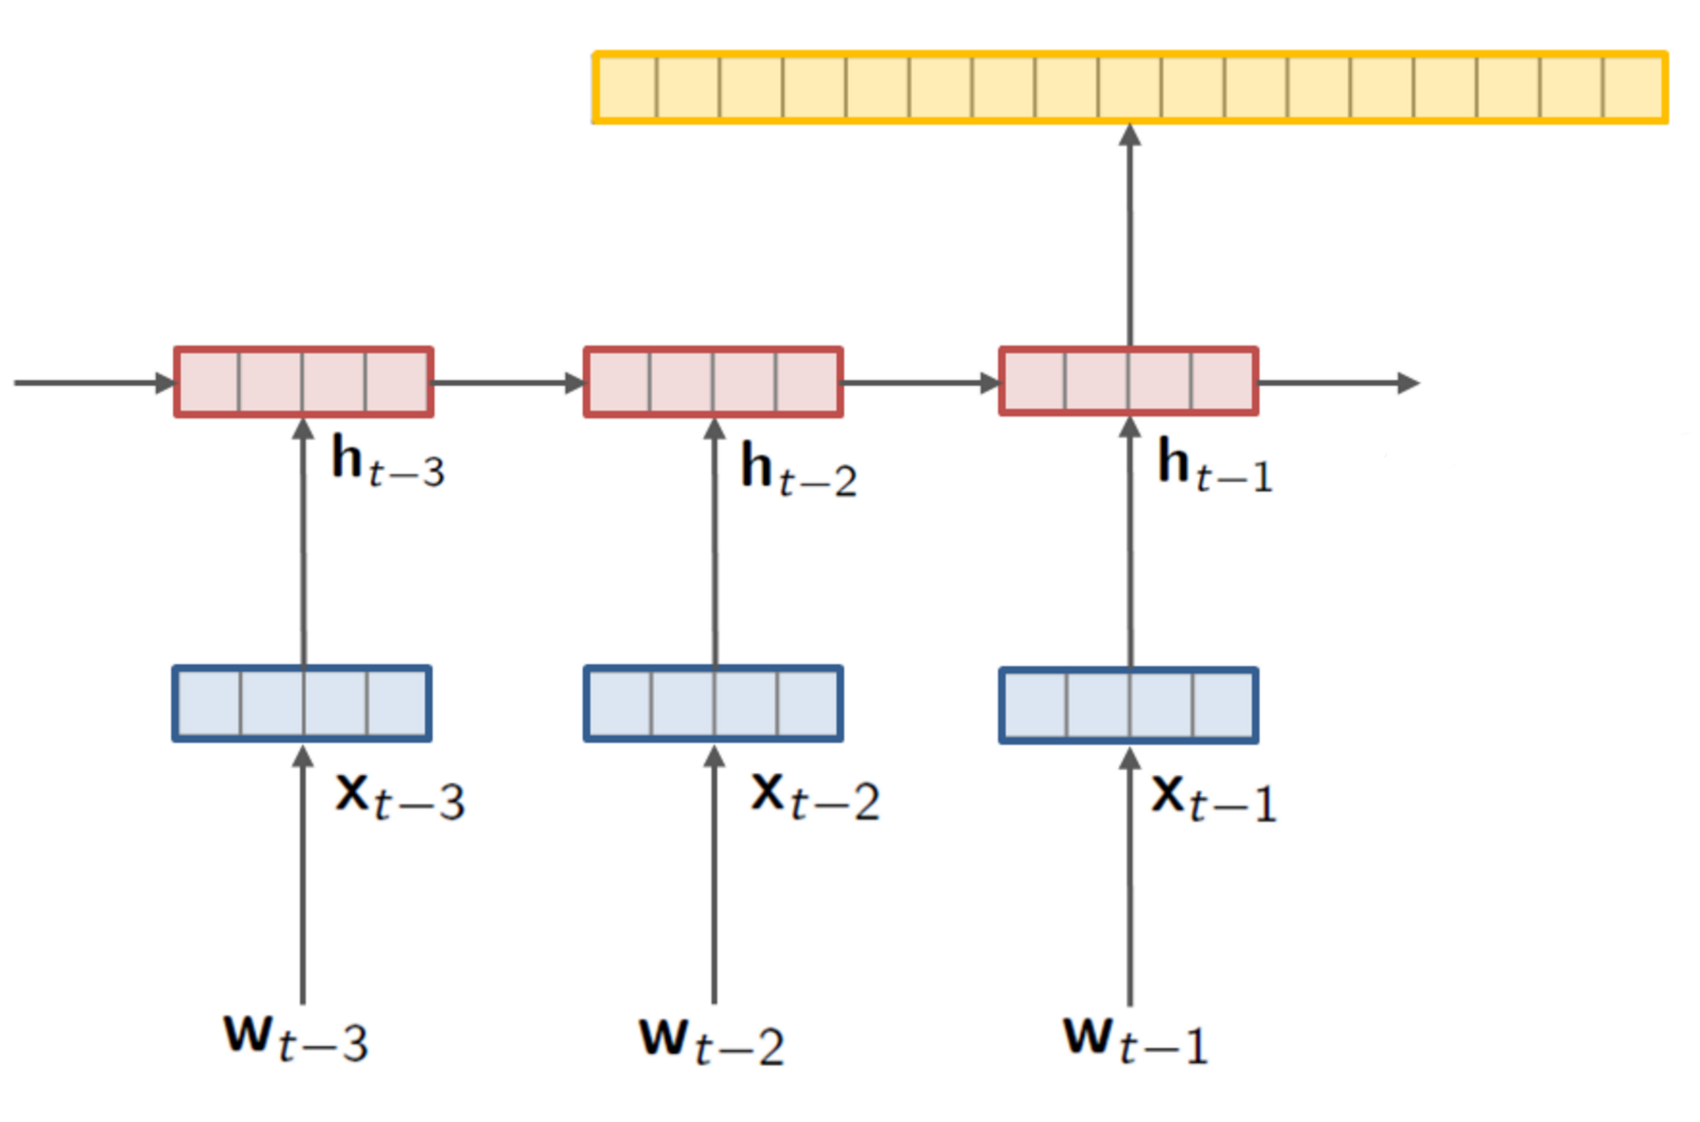
\includegraphics[width=3cm]{rnnlm6}};
%     \node[draw,  thick, rounded corners, scale=0.5] (ana) at (-15mm, 15mm) {Analysis};
%     \node[draw,  fill=yellow, thick, rounded corners,scale=0.5] (meth) at (0mm, 30mm) {\ Methods\phantom{p}};
%     \node[draw,  thick, rounded corners,scale=0.5] (app) at (25mm, 30mm) {Applications};
%     \node[draw, thick, rounded corners, scale=0.5] (und) at (35mm, 15mm) {Understanding};
%     \node[draw, fill=yellow, thick, rounded corners, scale=0.5] (dep) at (25mm, 0mm){Deployment};

%     \node[draw, thick, rounded corners,scale=0.5] (imp) at (0, 0) {Implementation};

%     \draw (ana) -- (meth) --(app) -- (und) -- (dep) -- (imp) -- (ana);

%   \end{tikzpicture}
% }
%   \end{center}
% \end{frame}


\begin{frame}{Beam Search Optimization}
  Research Goal: Can we learn parameters $\theta$ to target text generation problems?

    \[ {y^*_{1:T}} = \argmax_{y_{\tikzmark{opt}1:T}} {f_{\theta}}(y_{1:T}, \tikzmark{input}{x}) \]


  \begin{itemize}

  \item Input {$x$},  \textit{what to talk about}
    \air

  \item Output text {$y^*_{1:T}$}, \textit{how to say it}
    \air

  \item Scoring model {$f_\theta$}
  \end{itemize}

\end{frame}


\begin{frame}{Training Encoder-Decoder}
  Parameters $\theta$ are trained to score the next word given the \textit{true} history, $\hat{y}_{1:t-1}$

  \begin{center}
  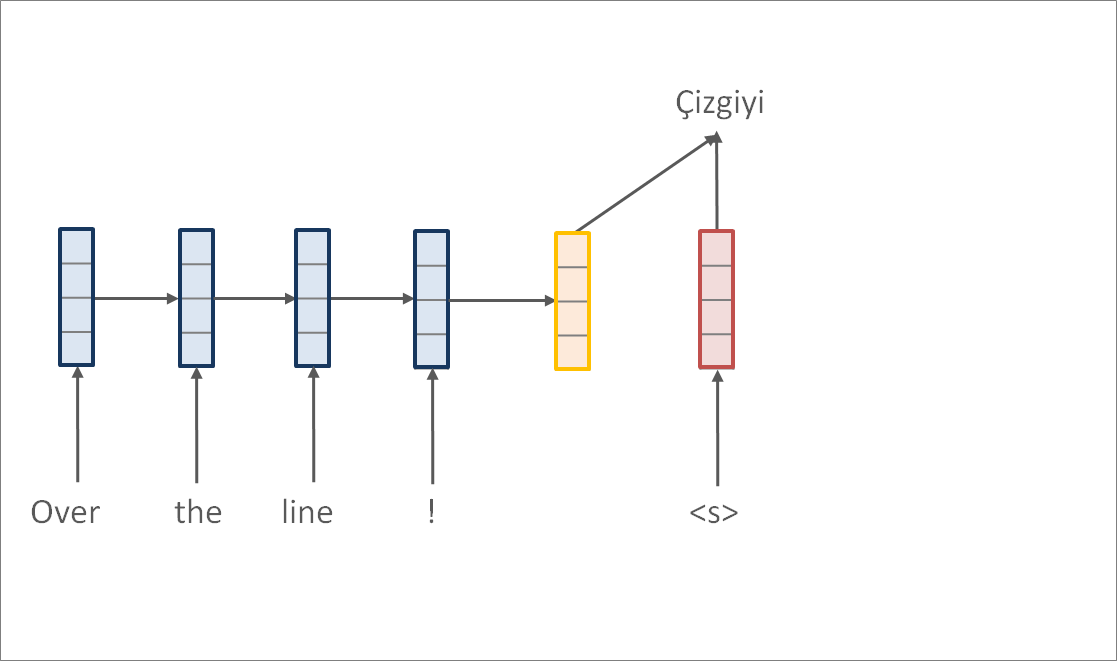
\includegraphics[height=3.5cm, trim={12cm 3cm 7cm 0.5cm}, clip]{nmt-noattn-4}
  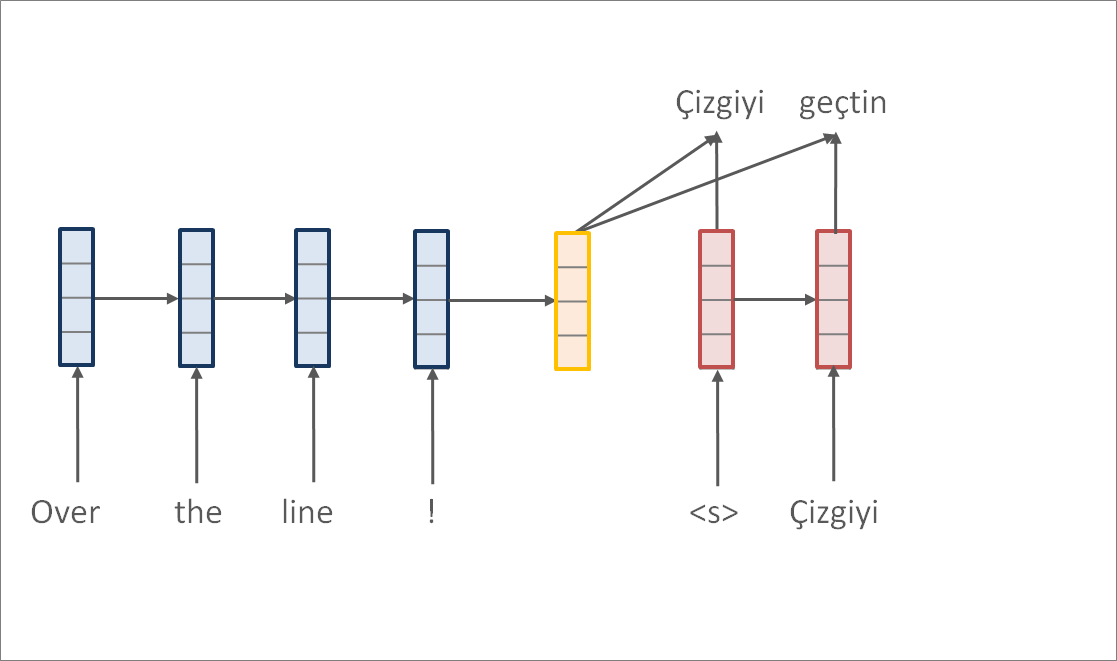
\includegraphics[height=3.5cm, trim={12cm 3cm 3cm 0.5cm}, clip]{nmt-noattn-6}
  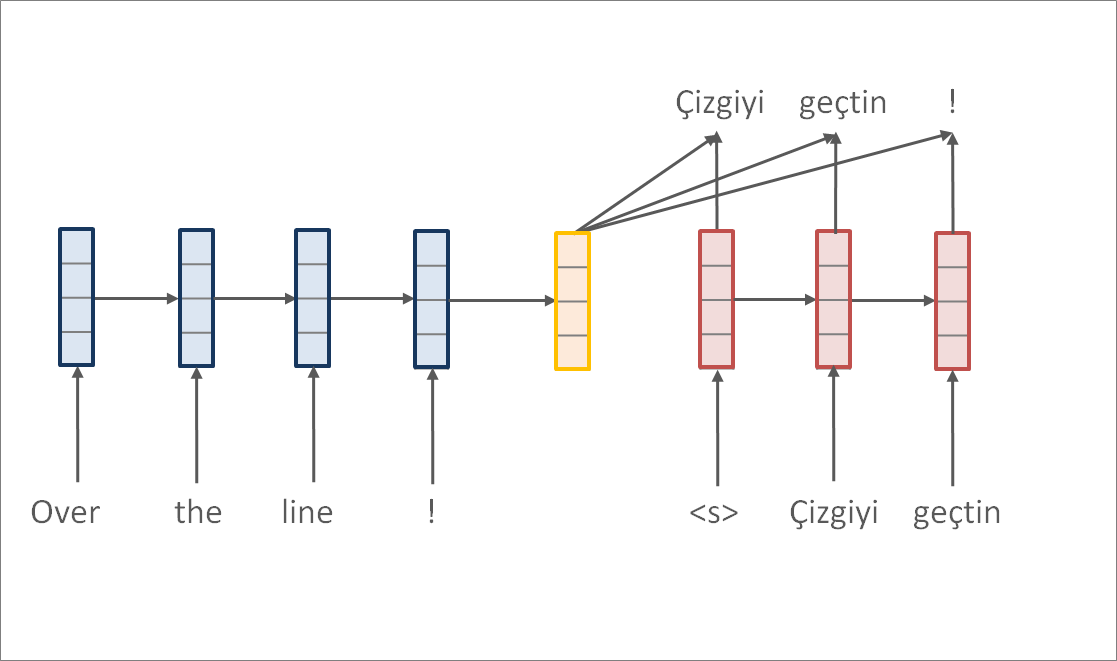
\includegraphics[height=3.5cm, trim={12cm 3cm 0.5cm 0.5cm}, clip]{nmt-noattn-7}
  % 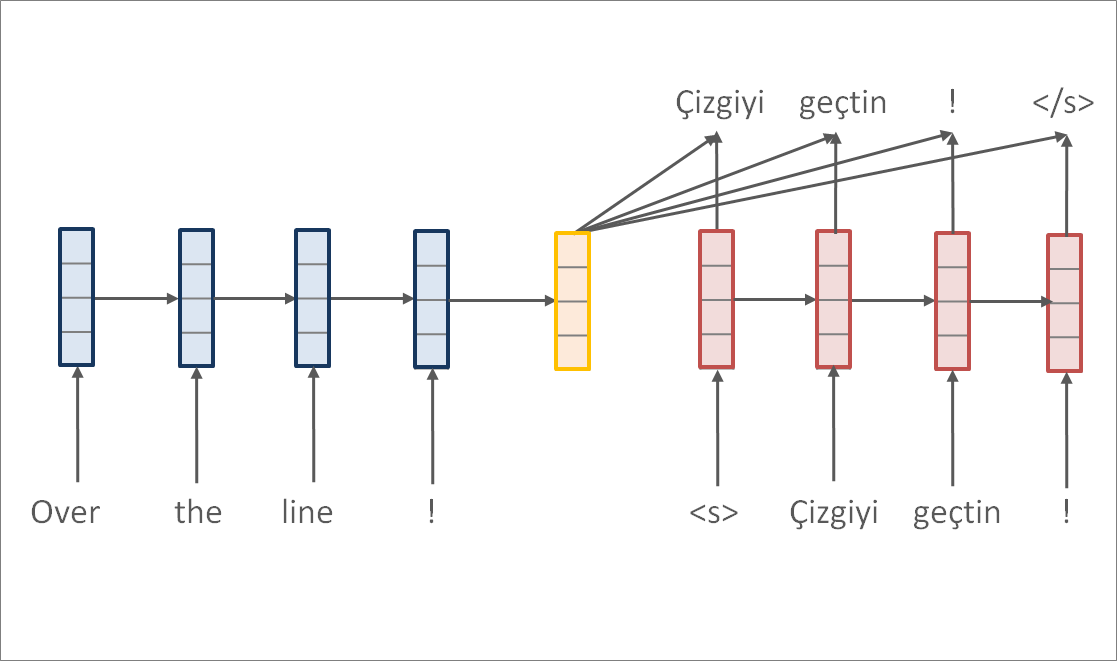
\includegraphics[height=3.5cm, trim={12cm 3cm 0.5cm 0.5cm}, clip]{nmt-noattn-8}
  \end{center}
  \pause

  Training loss is identical to \textcolor{redpurple}{multiclass classification} 
  \[ {\cal L}(\theta) = -\sum_{t} \log p(y_t |  \hat{y}_{1:t-1}, x; \theta) \]
\end{frame}

\begin{frame}{Generating with Encoder-Decoder}
  Parameters $\theta$ are used to score the next word given \textit{any} history, $y_{1:t-1}$.


  \begin{center}
  % 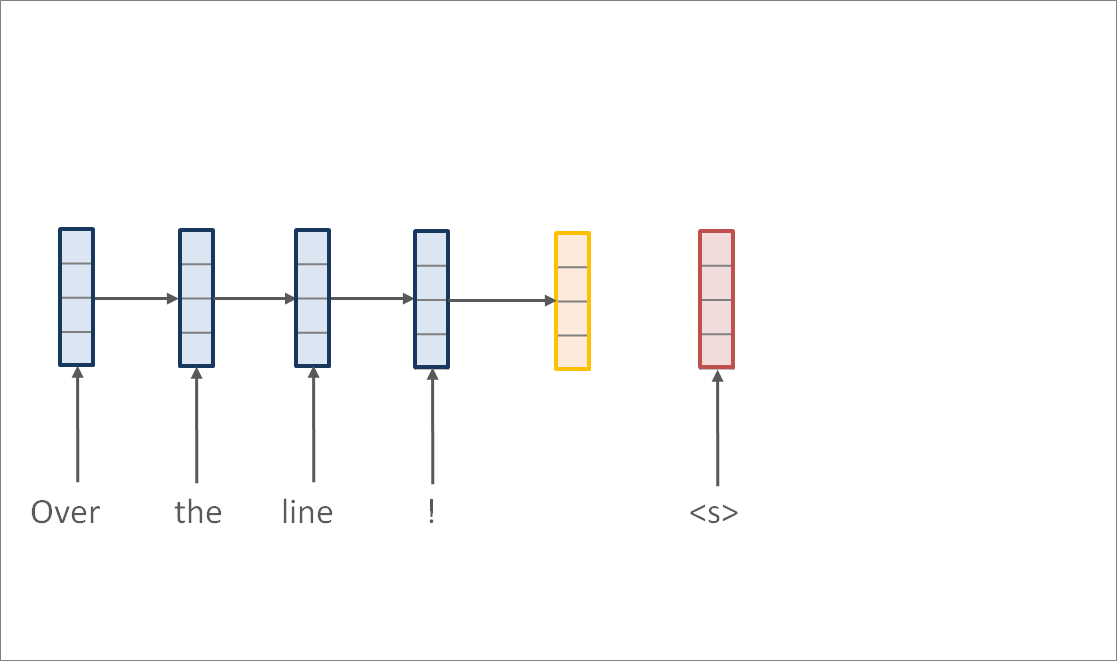
\includegraphics[height=3.5cm, trim={12cm 3cm 7cm 0.5cm}, clip]{nmt-noattn-3}
  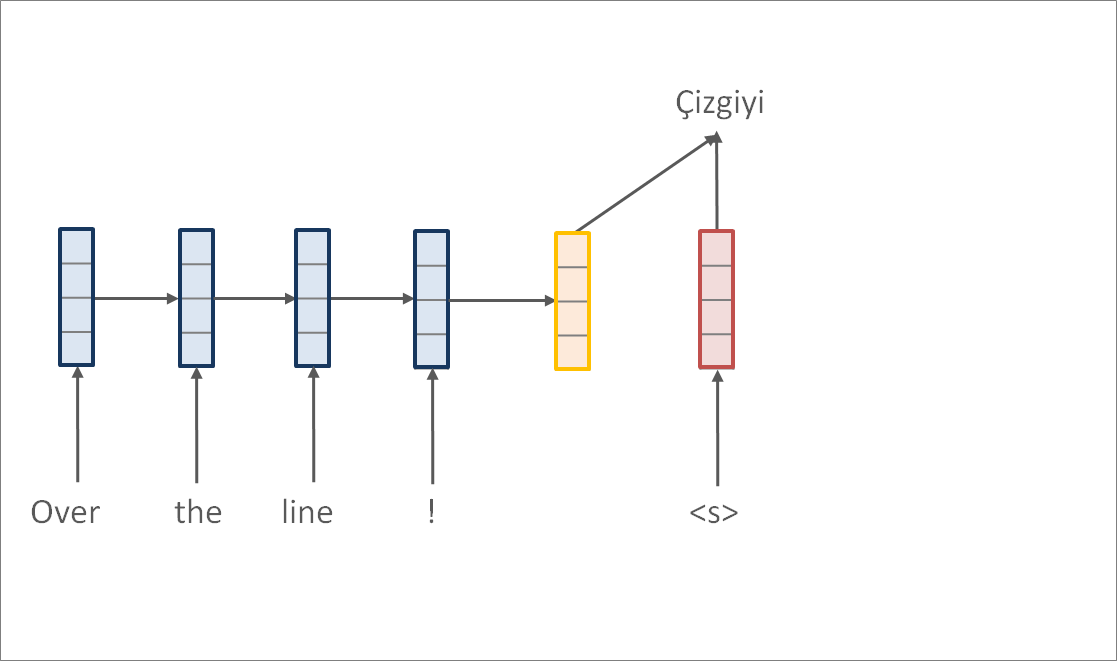
\includegraphics[height=3.5cm, trim={12cm 3cm 7cm 0.5cm}, clip]{nmt-noattn-4}
  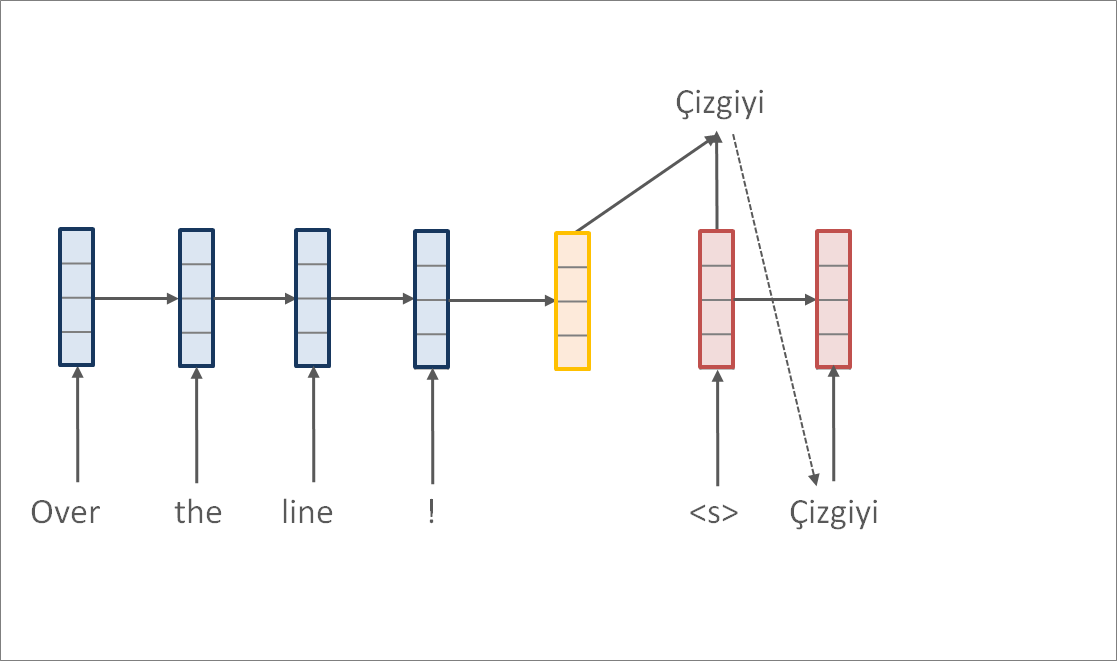
\includegraphics[height=3.5cm, trim={12cm 3cm 0.5cm 0.5cm}, clip]{nmt-noattn-5}
  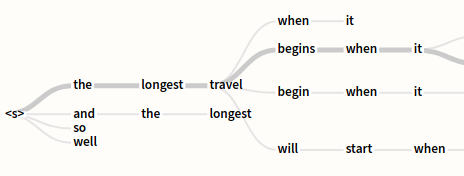
\includegraphics[width=7cm]{beam}
  \end{center}

  Generation aims to maximize over all sequences,
  \[ y^*_{1:T} =d \argmax_{y_{1:T}} f_{\theta}(y_{1:T}, x) = \argmax_{y_{1:T}} \sum_{t} \log p(y_{t} | y_{1:t-1}, x; \theta) \]
  % \pause
  % Intractable to solve exactly $O(\text{\#vocab} ^T)$

\end{frame}

\begin{frame}[fragile]{Standard Heuristic Method:  Beam Search}
  {$ y^*_{1:T} \approx \argmax_{y_{1:T}} f_{\theta}(y_{1:T}, x)$ }

  \air 

    \begin{center}
  \begin{tikzpicture}[transform canvas = {scale=0.8}]
    \tikzstyle{beam}=[draw, minimum height=0.6cm, anchor=base, text height=5, text depth=0, minimum width=1.5cm,thin, rounded corners, line width=0.03cm]
   \tikzstyle{mat}=[draw=white]
    \tikzset{>=stealth',every on chain/.append style={join},
      every join/.style={->}}


       \begin{scope}
   \matrix (G) [matrix of nodes, nodes={beam},inner sep=1mm,row sep=0.03cm, column sep=0.8cm ] {
    \node<1->(G-1-1){a}; & \node<2->(G-1-2){red}; & \node<3->(G-1-3){dog}; & \node<4->(G-1-4){smells}; & \node<5->(G-1-5){home};  & \node<6->(G-1-6){today}; \\
    \node<1->(G-2-1){the}; & \node<2->(G-2-2){dog}; & \node<3->(G-2-3){dog}; & \node<4->(G-2-4){barks}; & \node<5->(G-2-5){quickly}; & \node<6->(G-2-6){Friday}; \\
    \node<1->(G-3-1){red}; & \node<2->(G-3-2){blue}; & \node<3->(G-3-3){cat}; &  \node<4->(G-3-4){walks}; & \node<5->(G-3-5){straight}; & \node<6->(G-3-6){now}; \\    };

    \only<2->{
      \draw[->] (G-1-1.east) -> (G-1-2.west);
      \draw[->] (G-2-1.east) -> (G-2-2.west);
      \draw[->] (G-1-1.east) -> (G-3-2.west);
      \draw[double, line width=0.03cm] (G-3-1.south west) -- (G-3-2.south east);
    }

    \only<3->{
      \draw[->] (G-1-2.east) -> (G-2-3.west);
      \draw[->] (G-3-2.east) -> (G-3-3.west);
      \draw[->] (G-3-2.east) -> (G-1-3.west);
      \draw[double, line width=0.03cm] (G-3-1.south west) -- (G-3-3.south east);
    }

 \only<4->{
    \draw[->] (G-1-3.east) -> (G-3-4.west);
    \draw[->] (G-2-3.east) -> (G-2-4.west);
    \draw[->] (G-1-3.east) -> (G-1-4.west);
    \draw[double, line width=0.03cm] (G-3-1.south west) -- (G-3-4.south east);
}
 \only<6->{
    \draw[->] (G-1-5.east) -> (G-1-6.west);
    \draw[->] (G-1-5.east) -> (G-3-6.west);
    \draw[->] (G-2-5.east) -> (G-2-6.west);
    \draw[double, line width=0.03cm] (G-3-1.south west) -- (G-3-6.south east);
}

 \only<5->{
    \draw[->] (G-3-4.east) -> (G-1-5.west);
    \draw[->] (G-3-4.east) -> (G-2-5.west);
    \draw[->] (G-3-4.east) -> (G-3-5.west);
    \draw[double, line width=0.03cm] (G-3-1.south west) -- (G-3-5.south east);
}
         \node[yshift=0.7cm, left=0.2cm of G]{k = 1};
         \node[left=0.2cm of G]{k = 2};
         \node[yshift=-0.7cm, left=0.2cm of G]{k = 3};
         \node[below=0.1cm of G]{t};

\end{scope}
\end{tikzpicture}
    \end{center}

\air
    \air

\air

\visible<7->{
   \begin{enumerate}
   \item Compute the score of every hypothesis $k$ and possible next word $y_t$, 
     \[f_{\theta}(\langle y_t, y_{1:t-1}^{(k)}\rangle, x) \gets \log p(y_{t}\ |\ y^{(k)}_{1:t-1}, x) + \log p(y^{(k)}_{1:t-1} \ |\  x) \]
     \pause
   \item Prune to only the $K$ highest-scoring of ($K \times \text{vocab}$) choices, 
     \[y_{1:t}^{(1:K)} \gets K\argmax_{y_t, k} f_{\theta}(\langle y_t, y_{1:t}^{(k)} \rangle, x)\]
   \end{enumerate}
}

  % \begin{enumerate}
  % \item Start with $K$ partial starting hypotheses $\wvec^{(1:K)}$
  % \item For timesteps $t$ from  $1$ to $T$:
  %  \begin{enumerate}
  %  \item Compute for all $k, \wvec_{t}$
  %    \[s(\wvec_t, k) \gets \log p(\wvec_{t} | \wvec^{(k)}_{1:t-1}, \cvec; \theta) + \log p(\wvec^{(k)}_{1:t-1}| \cvec;\theta) \]
  %  \item Save $K$ highest scoring target sequences
  %    \[\wvec_{1:t+1}^{(1:K)} \gets K\arg\max_{\wvec_t, k} s(\wvec_t, k)\]
  %  \end{enumerate}
  % \end{enumerate}
  \pause
  % \begin{itemize}
  % \item Note: Requires computing $p(\wvec_{t} | \wvec^{(k)}_{1:t-1}, \cvec; \theta)$ for many  $\wvec^{(k)}_{1:t-1}$
  % \end{itemize}
\end{frame}

% \begin{frame}[fragile]{Beam Search Example} ($K=3$)


%     \begin{center}
%   \begin{tikzpicture}[transform canvas = {scale=0.8}]
%     \tikzstyle{beam}=[draw, minimum height=0.6cm, anchor=base, text height=5, text depth=0, minimum width=1.5cm,thin, rounded corners, line width=0.03cm]
%    \tikzstyle{mat}=[draw=white]
%     \tikzset{>=stealth',every on chain/.append style={join},
%       every join/.style={->}}


%        \begin{scope}

%    \matrix (G) [matrix of nodes, nodes={beam},inner sep=1mm,row sep=0.03cm, column sep=0.8cm ] {
%     \node<1->(G-1-1){a}; & \node<2->(G-1-2){red}; & \node<3->(G-1-3){dog}; & \node<4->(G-1-4){smells}; & \node<5->(G-1-5){home};  & \node<6->(G-1-6){today}; \\
%     \node<1->(G-2-1){the}; & \node<2->(G-2-2){dog}; & \nodek<3->(G-2-3){dog}; & \node<4->(G-2-4){barks}; & \node<5->(G-2-5){quickly}; & \node<6->(G-2-6){Friday}; \\
%     \node<1->(G-3-1){red}; & \node<2->(G-3-2){blue}; & \node<3->(G-3-3){cat}; &  \node<4->(G-3-4){runs}; & \node<5->(G-3-5){straight}; & \node<6->(G-3-6){now}; \\    };

%     \only<2->{
%       \draw[->] (G-1-1.east) -> (G-1-2.west);
%       \draw[->] (G-2-1.east) -> (G-2-2.west);
%       \draw[->] (G-1-1.east) -> (G-3-2.west);
%       \draw[double, line width=0.03cm] (G-3-1.south west) -- (G-3-2.south east);
%     }

%     \only<3->{
%       \draw[->] (G-1-2.east) -> (G-2-3.west);
%       \draw[->] (G-3-2.east) -> (G-3-3.west);
%       \draw[->] (G-3-2.east) -> (G-1-3.west);
%       \draw[double, line width=0.03cm] (G-3-1.south west) -- (G-3-3.south east);
%     }

%  \only<4->{
%     \draw[->] (G-1-3.east) -> (G-3-4.west);
%     \draw[->] (G-2-3.east) -> (G-2-4.west);
%     \draw[->] (G-1-3.east) -> (G-1-4.west);
%     \draw[double, line width=0.03cm] (G-3-1.south west) -- (G-3-4.south east);
% }
%  \only<6->{
%     \draw[->] (G-1-5.east) -> (G-1-6.west);
%     \draw[->] (G-1-5.east) -> (G-3-6.west);
%     \draw[->] (G-2-5.east) -> (G-2-6.west);
%     \draw[double, line width=0.03cm] (G-3-1.south west) -- (G-3-6.south east);
% }

%  \only<5->{
%     \draw[->] (G-3-4.east) -> (G-1-5.west);
%     \draw[->] (G-3-4.east) -> (G-2-5.west);
%     \draw[->] (G-3-4.east) -> (G-3-5.west);
%     \draw[double, line width=0.03cm] (G-3-1.south west) -- (G-3-5.south east);
% }

% \end{scope}
% \end{tikzpicture}
%     \end{center}
%     \air

% For timesteps $t$ from  $1$ to $T$:
%    \begin{enumerate}
%    \item Compute for all $k, \wvec_{t}$
%      \[f(\wvec_t, \wvec_{1:t-1}^{(k)}) \gets \log p(\wvec_{t} | \wvec^{(k)}_{1:t-1}, \cvec) + \log p(\wvec^{(k)}_{1:t-1}| \cvec) \]
%    \item Replace the $K$ highest scoring target sequences
%      \[\wvec_{1:t}^{(1:K)} \gets K\argmax_{\wvec_{1:t}} (\wvec_t, \wvec_{1:t-1}^{(k)})\]
%    \end{enumerate}

% \end{frame}


\begin{frame}{Core Issue}

  \begin{center}
    Multiclass Training $\Rightarrow$ Structured Generation ?
  \end{center}

  \pause
  \begin{enumerate}
  \item Exposure Bias
    \begin{itemize}
    \item Training conditions on true history, but generation uses predicted history.
    \end{itemize}
    \air
    \pause

  \item Label Bias  %\cite{Lafferty2001}
    \begin{itemize}
    \item Training is locally multiclass, but score is over entire sequences.
    \end{itemize}
    \air
    \pause


  \item Metric Bias
    \begin{itemize}
    \item Training uses multiclass classification, but evaluation uses n-gram match.
    \end{itemize}
    \air

  \end{enumerate}
\end{frame}

% \begin{frame}{Beam Search Optimization}

%   \textbf{Strategy:} Modify training to target each issue.

%   \begin{itemize}
%   \item Exposure Bias, Label Bias, Metric Bias

%   \end{itemize}
% \air
% \air

%   \textbf{Applications:}

%   \begin{enumerate}
%   \item Improvements in training with less supervision.
%     \air
%   \item  Effective methods for downscaling translation models.
%     \air
%   \end{enumerate}
% \end{frame}


% \begin{frame}{\structure{Related Work:} Modify training data}
%   \air
%   \begin{itemize}
%   \item Data as Demonstrator \Cite{Venkatraman}, Scheduled Sampling \Cite{Bengio2015}
%   \end{itemize}
%   \air

%   \centerline{\structure{Related Work:} Use Reinforcement Learning}
%   \air
%   \begin{itemize}
%   \item MIXER \Cite{Ranzato2016}
%   \item Actor-Critic \Cite{Bahdanau2016}
%   \end{itemize}

%   \pause

%   Opinion:
%   \begin{itemize}
%   \item
%     DAD methods only address exposure bias,
%   \item RL is too strong a hammer .
%   \end{itemize}

%   % \begin{itemize}
%   % \item
%   % \end{itemize}
% \end{frame}

% \begin{frame}{Sequence-to-Sequence Learning as Beam Search Optimization}


%   Proposal: Directly modify the RNN training procedure to fix test biases.


%   % \begin{itemize}
%   % \item
%   % \end{itemize}
% \end{frame}

\begin{frame}{Modification 1: Beam Search at Training}

  \textbf{Fix:} Exposure Bias
    \begin{itemize}
    \item Take prediction algorithm into account during training.
    \end{itemize}
    \air
    \pause

   \begin{center}
     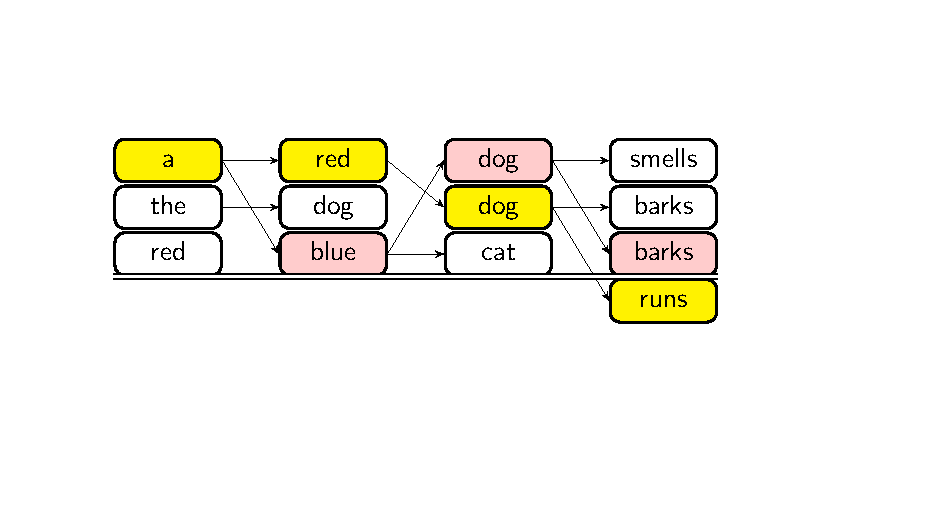
\includegraphics[width=8cm, clip, trim={0cm 3cm 0cm 1cm}]{out-4}
   \end{center}
   \begin{itemize}
   \item Run our beam search procedure during training (structured training)
     \air

   \item Loss tied to  mistakes, e.g. true sequence $\hat{y}_{1:t}$ is \textit{violated} by $y^{(K)}_{1:t}$ worst beam 
   \end{itemize}
   % \begin{enumerate}
   % \item Compute the score of every possible next word.

   %   \[f(y_t, y_{1:t-1}^{(k)}) \gets \log p(y_{t}\ |\ y^{(k)}_{1:t-1}, x) + \log p(y^{(k)}_{1:t-1} \ |\  x) \]

   % % \only<2>{
   % %   \[f(y_t, y_{1:t-1}^{(k)})  \gets  \structure{f(y_t, y_{1:t-1}^{(k)}, x; \theta)} \]}

   % \item Prune to only the $K$ highest-scoring,
   %   \[y_{1:t}^{(1:K)} \gets K\argmax_{y_{1:t}} f(y_t, y_{1:t-1}^{(k)})\]
   % \end{enumerate}
  % \begin{enumerate}
  % % \item Start with $K$ partial starting hypotheses $\wvec^{(1:K)}$
  % % \item For timesteps $t$ from  $1$ to $T$:
  %  \begin{enumerate}
  %  \item Compute for all $k, \wvec_{t}$
  %    \only<1>{
  %    \[f(\wvec_t, \wvec_{1:t-1}^{(k)}) \gets \alert{\log p(\wvec_{t} | \wvec^{(k)}_{1:t-1}, \cvec; \theta) + \log p(\wvec^{(k)}_{1:t-1}| \cvec;\theta)} \]
  %  }
  %  \only<2>{
  %    \[f(\wvec_t, \wvec_{1:t-1}^{(k)})  \gets  \structure{f(\wvec_t, \wvec_{1:t-1}^{(k)}, \cvec; \theta)} \]
  %  }
  %  \item Replace the  $K$ highest scoring target sequences
  %    \[\wvec_{1:t}^{(1:K)} \gets K\argmax_{\wvec_{1:t}} s(\wvec_t, \wvec_{1:t-1}^{(k)})\]
  %  \end{enumerate}
  % \end{enumerate}
\end{frame}

\begin{frame}{Modification 2: Global Scoring Function  }
  \textbf{Fix:}  Label Bias
    \begin{itemize}
    \item Use a global sequence scoring function.
    \end{itemize}
    \pause

  % \begin{center}
  %   % \structure{(Idea 1)} Replace local softmax with sequence scorer
  %   % \air
  %
  % \end{center}

    \air

  % \textbf{Proposed Fix:}
  \begin{center}
    $f(y_{1:t}, x; \theta)= \mathbf{W} [\mathbf{h}_{t-1}; \mathbf{c}]$

    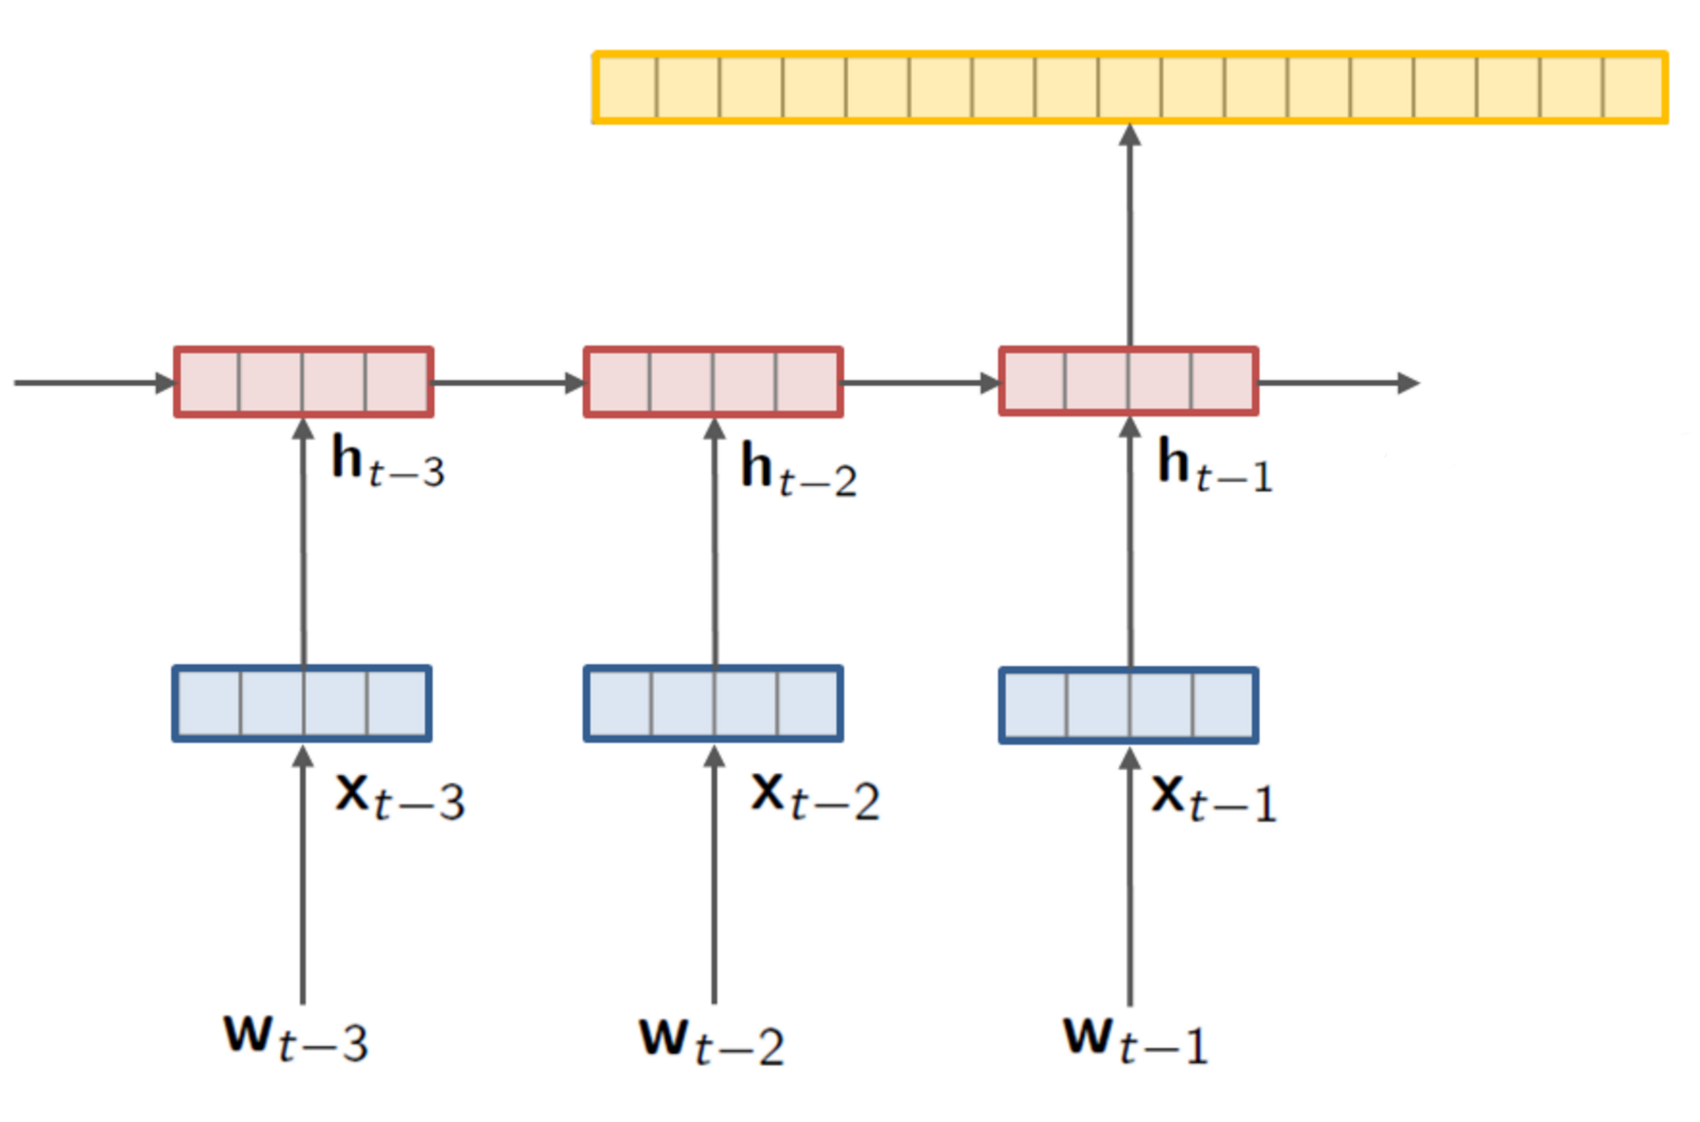
\includegraphics[width=0.5\textwidth, trim={0cm 18cm 0cm 0cm}, clip]{rnnlm6}
  \end{center}


  \begin{itemize}
  \item Replace local $ \log p(y_{t} | y_{1:t-1}, x; \theta)$ with
    a global scoring model $f_{\theta}(y_{1:t}, x)$.
  \end{itemize}
  \air


  
\end{frame}



\begin{frame}{Modification 3: Train with Margin}
  
  \textbf{Fix:} Metric Bias
  \begin{itemize}
  \item Incorporate a metric specific $\Delta$ term, e.g. n-gram mismatch
  \end{itemize}
  \air
  \pause
  
  \[ \mathcal{L}(\theta) = \sum_{t} \Delta(\hat{y}_{1:t}, y_{1:t}^{(K)}) \left[1 - f( \hat{y}_{1:t}, x; \theta) +  f(y_{1:t}^{(K)}, x;\theta) \right] \]
  
  \begin{itemize}
  \item Loss if true sequence $\hat{y}_{1:t}$ falls within a margin of worst beam sequence $y^{(K)}_{1:t}$
  \item Slack-rescaled margin takes problem-specific $\Delta$ into account
  \end{itemize}
  
\end{frame}

\begin{myverbbox}{\sTW}
 { \cal K } ^ { L } ( \sigma = 2 ) = \left( \begin{array}
{ c c } { - \frac { d ^ { 2 } } { d x ^ { 2 } } + 4 - \frac
 { 3 } { \operatorname { c o s h } ^ { 2 } x } } \& { \frac
 { 3 } { d x ^ { 2 } } }  { \frac { 3 } { \operatorname
 { c o s h } ^ { 2 } x } } \& { - \frac { d ^ { 2 } }
{ d x ^ { 2 } } + 4 - \frac { 3 } { \operatorname { c o s h }
^ { 2 } x } }  \end{array} \right) \qquad
\end{myverbbox}

\begin{frame}{Extension: Training with Hard Constraints}
  

  \textbf{Bonus:} Hard Constraints

  \begin{itemize}
  \item Beam Search Optimization allows users to enforce hard constraints at training. 
  \end{itemize}

  \textbf{Example:} Code generation with a known grammar,
    \begin{center}
      \begin{tikzpicture}
        \node (b)[xshift=6cm, rectangle, scale=0.6,
        draw,thick,fill=blue!0,text width=32em, rounded corners, inner
        sep =5pt, minimum height=1em]{\baselineskip=50pt \footnotesize
          \sTW };

    \end{tikzpicture}
  \end{center}

\end{frame}




\begin{frame}[fragile]{Beam Search Optimization: Training Example}
  \begin{center}
    \begin{center}

    \end{center}
    \air
    \air
    \air
    \air

\

  \begin{tikzpicture}[transform canvas = {scale=0.8}]
  \tikzstyle{beam}=[draw, minimum height=0.6cm, anchor=base, text height=5, text depth=0, minimum width=1.5cm,thin, rounded corners, line width=0.03cm]
  \tikzstyle{mat}=[draw=white]
\tikzset{>=stealth',every on chain/.append style={join},
         every join/.style={->}}


       % \node[draw = white, yshift=1.8cm]{Time Step};
       %\node[draw = white, xshift=-7.5cm, yshift=0.5cm]{Beam:};
       \begin{scope}


   \matrix (G) [matrix of nodes, nodes={beam},inner sep=1mm,row sep=0.03cm, column sep=0.8cm ] {
    \node<1->[fill=yellow](G-1-1){\textcolor{black}{a}}; \node<4->[fill=yellow](G-1-1){\textcolor{black}{a}}; & \node<2->[fill=yellow](G-1-2){red}; \node<4->[fill=yellow](G-1-2){red}; & \node<3->[](G-1-3){\textcolor{black}{dog}}; \node<4->[fill=red!20](G-1-3){\textcolor{black}{dog}}; & \node<4->(G-1-4){smells}; & \node<5->[](G-1-5){{home}}; \node<6->[fill=red!20](G-1-5){{home}};  & \node<6->[](G-1-6){{today}}; \\
    \node<1->(G-2-1){the}; & \node<2->(G-2-2){dog}; & \node<3->[fill=yellow](G-2-3){dog}; & \node<4->(G-2-4){barks}; & \node<5->[fill=yellow](G-2-5){quickly}; & \node<6->(G-2-6){Friday}; \\
    \node<1->(G-3-1){red}; & \node<2->[](G-3-2){\textcolor{black}{blue}}; \node<4->[fill=red!20](G-3-2){\textcolor{black}{blue}}; & \node<3->(G-3-3){cat}; &  \node<4->[fill=red!20](G-3-4){\textcolor{black}{barks}}; & \node<5->(G-3-5){straight}; & \node<6->[fill=red!20](G-3-6){now}; \\
    & & & \node<4->[fill=yellow](G-4-4){runs}; & & \node<6->[fill=yellow](G-4-6){today}; \\
    };

    \only<2->{
      \draw[->] (G-1-1.east) -> (G-1-2.west);
      \draw[->] (G-2-1.east) -> (G-2-2.west);
      \draw[->] (G-1-1.east) -> (G-3-2.west);
      \draw[double, line width=0.03cm] (G-3-1.south west) -- (G-3-2.south east);
    }

    \only<3->{
      \draw[->] (G-1-2.east) -> (G-2-3.west);
      \draw[->] (G-3-2.east) -> (G-3-3.west);
      \draw[->] (G-3-2.east) -> (G-1-3.west);
      \draw[double, line width=0.03cm] (G-3-1.south west) -- (G-3-3.south east);
    }

 \only<4->{
    \draw[->] (G-2-3.east) -> (G-4-4.west);
    \draw[->] (G-1-3.east) -> (G-3-4.west);
    \draw[->] (G-2-3.east) -> (G-2-4.west);
    \draw[->] (G-1-3.east) -> (G-1-4.west);
    \draw[double, line width=0.03cm] (G-3-1.south west) -- (G-3-4.south east);
}
 \only<6->{
    \draw[->] (G-1-5.east) -> (G-1-6.west);
    \draw[->] (G-1-5.east) -> (G-3-6.west);
    \draw[->] (G-2-5.east) -> (G-2-6.west);
    \draw[->] (G-2-5.east) -> (G-4-6.west);
    \draw[double, line width=0.03cm] (G-3-1.south west) -- (G-3-6.south east);
}

    % \draw[->] (G-3-2.east) -> (G-3-3.west);
    % \draw[->] (G-3-2.east) -> (G-1-3.west);

 \only<5->{
    \draw[->, dashed] (G-4-4.east) -> (G-1-5.west);
    \draw[->, dashed] (G-4-4.east) -> (G-2-5.west);
    \draw[->, dashed] (G-4-4.east) -> (G-3-5.west);
    \draw[double, line width=0.03cm] (G-3-1.south west) -- (G-3-5.south east);
}

       \end{scope}
    % \draw(G-1-1.north east) rectangle (G-3-1.south west);
    % \draw(G-1-2.north east) rectangle (G-3-2.south west);

    % \begin{scope}[yshift=-2.8cm]

    %   \matrix (G) [matrix of nodes,nodes={beam}, inner sep=1mm,row sep=0.06cm,column sep=0.8cm ] {
    %     \node[fill=yellow](G-1-1){a}; & \node[fill=yellow](G-1-2){red}; & \node[fill=yellow](G-1-3){dog}; & \node[fill=yellow](G-1-4){runs}; & \node[fill=yellow](G-1-5){quickly}; & \node[fill=yellow](G-1-6){today}; \\
    %      & \node[fill=lightgray](G-2-2){\textcolor{blue}{blue}}; & \node[fill=lightgray](G-2-3){\textcolor{blue}{dog}}; & \node[fill=lightgray](G-2-4){\textcolor{blue}{barks}}; & \node[fill=lightgray](G-2-5){\textcolor{red}{home}}; & \node[fill=lightgray](G-2-6){\textcolor{red}{today}}; \\
    %   };
    % \draw[->] (G-1-1.east) -> (G-1-2.west);
    % \draw[->] (G-1-2.east) -> (G-1-3.west);
    % \draw[->] (G-1-3.east) -> (G-1-4.west);
    % \draw[->] (G-1-4.east) -> (G-1-5.west);
    % \draw[->] (G-1-5.east) -> (G-1-6.west);

    % \draw[->] (G-1-1.east) -> (G-2-2.west);
    % \draw[->] (G-2-2.east) -> (G-2-3.west);
    % \draw[->] (G-2-3.east) -> (G-2-4.west);
    % \draw[->] (G-1-4.east) -> (G-2-5.west);
    % \draw[->] (G-2-5.east) -> (G-2-6.west);

    % \end{scope}
\end{tikzpicture}
  \end{center}
  \air
  \air
  \air
% \begin{align*}
%  \mathcal{L}&(\theta) = \sum_{t} \Delta(\wvec_{1:t}, \wvec_{1:t}^{(K)}) \left[1 - f(\wvec_t, \wvec_{1:t-1}, \cvec) +  f(\wvec_t^{(K)}, \wvec_{1:t-1}^{(K)}, \cvec) \right]
% \end{align*}

  \begin{itemize}
  \item \textcolor{orange}{True}: ground-truth sequence $\hat{y}_{1:t}$
  \item<4-> \textcolor{red}{Predicted}: lowest-scoring violating sequence  $y_{1:t}^{(K)}$
  \end{itemize}
  % Strategy: if true falls off beam, restart from ground truth (learning as search optimization \cite{daume05learning})
\end{frame}

\begin{frame}[fragile]{Parameter Updates: Structured Backpropagation}
  \begin{center}

  \air
  \air



  \begin{tikzpicture}[transform canvas = {scale=0.8}]
    \tikzstyle{beam}=[draw, minimum height=0.6cm, anchor=base, text height=5, text depth=0, minimum width=1.5cm,thin, rounded corners, line width=0.03cm]
    \tikzstyle{mat}=[draw=white]
    \tikzset{>=stealth',every on chain/.append style={join},
      every join/.style={->}}


       % \node[draw = white, yshift=1.8cm]{Time Step};
       %\node[draw = white, xshift=-7.5cm, yshift=0.5cm]{Beam:};
       \begin{scope}


   \matrix (G) [matrix of nodes, nodes={beam},inner sep=1mm,row sep=0.03cm, column sep=0.8cm ] {
     \node[fill=yellow](G-1-1){\textcolor{blue}{a}}; & \node[fill=yellow](G-1-2){red}; & \node[fill=lightgray](G-1-3){\textcolor{blue}{dog}}; & \node(G-1-4){smells}; & \node[fill=lightgray](G-1-5){\textcolor{red}{home}};  & \node[fill=lightgray](G-1-6){\textcolor{red}{today}}; \\
     \node(G-2-1){the}; & \node(G-2-2){dog}; & \node[fill=yellow](G-2-3){dog}; & \node(G-2-4){barks}; & \node[fill=yellow](G-2-5){quickly}; & \node(G-2-6){Friday}; \\
     \node(G-3-1){red}; & \node[fill=lightgray](G-3-2){\textcolor{blue}{blue}}; & \node(G-3-3){cat}; &  \node[fill=lightgray](G-3-4){\textcolor{blue}{barks}}; & \node(G-3-5){straight}; & \node[](G-3-6){now}; \\
     & & & \node[fill=yellow](G-4-4){runs}; & & \node[fill=yellow](G-4-6){today}; \\
    };


    \draw[->] (G-1-1.east) -> (G-1-2.west);
    \draw[->] (G-2-1.east) -> (G-2-2.west);
    \draw[->] (G-1-1.east) -> (G-3-2.west);
    \draw[double, line width=0.03cm] (G-3-1.south west) -- (G-3-2.south east);


    \draw[->] (G-1-2.east) -> (G-2-3.west);
    \draw[->] (G-3-2.east) -> (G-3-3.west);
    \draw[->] (G-3-2.east) -> (G-1-3.west);
    \draw[double, line width=0.03cm] (G-3-1.south west) -- (G-3-3.south east);

    \draw[->] (G-2-3.east) -> (G-4-4.west);
    \draw[->] (G-1-3.east) -> (G-3-4.west);
    \draw[->] (G-2-3.east) -> (G-2-4.west);
    \draw[->] (G-1-3.east) -> (G-1-4.west);
    \draw[double, line width=0.03cm] (G-3-1.south west) -- (G-3-4.south east);

    \draw[->] (G-1-5.east) -> (G-1-6.west);
    \draw[->] (G-1-5.east) -> (G-3-6.west);
    \draw[->] (G-2-5.east) -> (G-2-6.west);
    \draw[->] (G-2-5.east) -> (G-4-6.west);
    \draw[double, line width=0.03cm] (G-3-1.south west) -- (G-3-6.south east);


    % \draw[->] (G-3-2.east) -> (G-3-3.west);
    % \draw[->] (G-3-2.east) -> (G-1-3.west);


    \draw[->, dashed] (G-4-4.east) -> (G-1-5.west);
    \draw[->, dashed] (G-4-4.east) -> (G-2-5.west);
    \draw[->, dashed] (G-4-4.east) -> (G-3-5.west);
    \draw[double, line width=0.03cm] (G-3-1.south west) -- (G-3-5.south east);


       \end{scope}


       \begin{scope}[yshift=-2.8cm]

      \matrix (G) [matrix of nodes,nodes={beam}, inner sep=1mm,row sep=0.06cm,column sep=0.8cm ] {
        \node[fill=yellow](G-1-1){a}; & \node[fill=yellow](G-1-2){red}; & \node[fill=yellow](G-1-3){dog}; & \node[fill=yellow](G-1-4){runs}; & \node[fill=yellow](G-1-5){quickly}; & \node[fill=yellow](G-1-6){today}; \\
         & \node[fill=lightgray](G-2-2){\textcolor{blue}{blue}}; & \node[fill=lightgray](G-2-3){\textcolor{blue}{dog}}; & \node[fill=lightgray](G-2-4){\textcolor{blue}{barks}}; & \node[fill=lightgray](G-2-5){\textcolor{red}{home}}; & \node[fill=lightgray](G-2-6){\textcolor{red}{today}}; \\
      };
    \draw[->] (G-1-1.east) -> (G-1-2.west);
    \draw[->] (G-1-2.east) -> (G-1-3.west);
    \draw[->] (G-1-3.east) -> (G-1-4.west);
    \draw[->] (G-1-4.east) -> (G-1-5.west);
    \draw[->] (G-1-5.east) -> (G-1-6.west);

    \draw[->] (G-1-1.east) -> (G-2-2.west);
    \draw[->] (G-2-2.east) -> (G-2-3.west);
    \draw[->] (G-2-3.east) -> (G-2-4.west);
    \draw[->] (G-1-4.east) -> (G-2-5.west);
    \draw[->] (G-2-5.east) -> (G-2-6.west);

    \end{scope}
  \end{tikzpicture}
  \end{center}
  \vspace{2cm}
  \vspace{1cm}

  % \begin{itemize}
  % \item Margin gradients are sparse, only grey sequences get updates.
  % \item Backprop as efficient as standard models.
  % \end{itemize}
\end{frame}

% \begin{frame}
%   \begin{center}
%     \structure{(Idea 3)} Extension: Incorporate hard constraints at training.
%   \end{center}

% \end{frame}

% \begin{frame}{Theoretical Issues Revisited}
%   \begin{itemize}

%   \item Exposure Bias
%     \begin{itemize}
%     \item Beam search at training
%     \end{itemize}
%     \air
%   \item Train/Test Loss Mismatch
%     \begin{itemize}
%     \item Slack-rescaled margin can capture correct loss.
%     \end{itemize}

%     \air
%   \item Label Bias  \cite{Lafferty2001}
%     \begin{itemize}
%     \item Sequence regression is not locally normalized
%     \end{itemize}

%   \end{itemize}
% \end{frame}


% \begin{frame}{Experiments}
%   \air

%   Experiments run on three different seq2seq baseline tasks

%   \begin{itemize}
%   \item Word Ordering
%     \air
%   \item Dependency Parsing
%     \air
%   \item Machine Translation
%   \end{itemize}



%   Details:
%   \begin{itemize}
%   \item Utilize our \textit{seq2seq-attn} code, very strong attention-based system
%   \item Pretrained with NLL.
%   \item Trained with a curriculum to gradually increase beam size.
%   \end{itemize}

% \end{frame}


\begin{frame}{Main Results}
  \vspace{-0.2cm}
  \begin{table}
  \centering
    \footnotesize
  \begin{tabular}{lccc}
    \toprule
    Train Beam & $K$ = 1 & $K$ = 5 & $K$ = 10 \\
    \midrule
     & \multicolumn{3}{c}{Word Ordering (BLEU) } \\
    \midrule
    Encoder-Decoder & 25.2 & 29.8 & 31.0 \\
    Beam Search Optimization     & 28.0 & 33.2 & 34.3 \\
    Beam Search Optimization-Constraints & \textbf{28.6} & \textbf{34.3} & \textbf{34.5} \\
    \midrule
    \pause
%   \end{tabular}
%   \label{tab:wo}
% \end{table}


% \begin{table}
%   \centering
%   \hspace*{-0.3cm}\begin{tabular}{lccc}
    % \toprule
    & \multicolumn{3}{c}{Dependency Parsing (UAS) } \\
    \midrule
    Encoder-Decode & \textbf{87.33} & 88.53 & 88.66\\
    Beam Search Optimization & 86.91 & 91.00 & 91.17 \\
    Beam Search Optimization-Constraints & 85.11 & \textbf{91.25} & \textbf{91.57} \\
    % \midrule
    % Andor & 93.17/91.18 & - & - \\
    % \bottomrule

    \midrule
    \pause
    & \multicolumn{3}{c}{Machine Translation (BLEU) } \\
    % &  $K_e$ = 1 & $K_e$ = 5 & $K_e$ = 10 \\
    \midrule
    Encoder-Decoder & 22.53 & 24.03 & 23.87 \\
    Beam-Search Optimization, $\Delta$  & \textbf{23.83} & \textbf{26.36} & \textbf{25.48} \\
    % \midrule
    % XENT & 17.74 & $\leq$ 20.5 & $\leq$ 20.5 \\
    % DAD & 20.12 & $\leq$ 22.5 & $\leq$ 23.0 \\
    % MIXER & 20.73 & - & $\leq$ 22.0 \\
    \bottomrule
  \end{tabular}
  \label{tab:mtfinal}
\end{table}

\end{frame}


% \begin{frame}

% \end{frame}

% \begin{frame}
%   \centerline{\structure{Related Work: Compressing Deep Models}}
% \air

% \begin{itemize}
% \item \textbf{Pruning}: Prune weights based on importance criterion
% \cite{LeCun1990,Han2016}
% \item \textbf{Knowledge Distillation}: Train a \textit{student} model to learn
% from a \textit{teacher} model \cite{Bucila2006,Ba2014,Hinton2015}.
% \end{itemize}
% \air
% Other methods:
% \begin{itemize}
% \item low-rank matrix factorization of weight matrices \cite{Denton2014}
% \item weight binarization \cite{Lin2016}
% \item weight sharing \cite{Chen2015}
% \end{itemize}
% \end{frame}



% \begin{frame}
% \centerline{\structure{Word-Level Knowledge Distillation}}
% \air
% \air

% \begin{columns}
% \begin{column}{6.5cm}
% Teacher network: $q(\yvec \given  ; \theta_T$)  \\
% \air
% \air
% Student network: $p(\yvec \given \xvec ; \theta$)
% \end{column}
% \begin{column}{5.5cm}
% 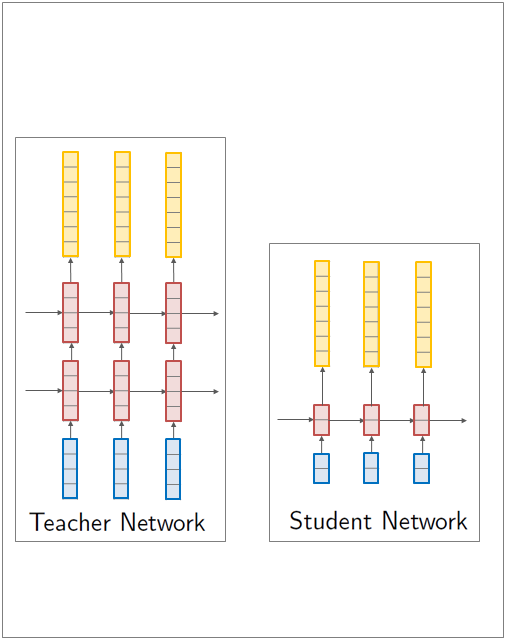
\includegraphics[width=5.5cm]{word-kd-1}
% \end{column}
% \end{columns}
% \end{frame}

% \begin{frame}
%   (Teacher-Student Diagram)
% \end{frame}

\begin{frame}{Application: Model Compression}
  \research{\cite{Kim2016a}}

  \textbf{Goal:} Shrink the size of text generation models.

% \begin{frame}
%   \centerline{\structure{Related Work: Compressing Deep Models}}
% \air

\begin{itemize}
% \item \textbf{Pruning}: Prune weights based on importance criterion
% \cite{LeCun1990,Han2016}
\item Knowledge Distillation: Train a \textit{student} model to learn
from a \textit{teacher} model. %\cite{Bucila2006,Ba2014,Hinton2015}.

\begin{center}
  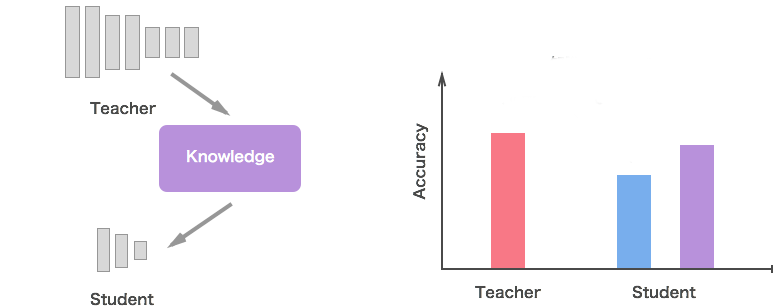
\includegraphics[width=10cm]{distill}
\end{center}
\end{itemize}



% \air
% Other methods:
% \begin{itemize}
% \item low-rank matrix factorization of weight matrices \cite{Denton2014}
% \item weight binarization \cite{Lin2016}
% \item weight sharing \cite{Chen2015}
% \end{itemize}
% \end{frame}



\end{frame}

% \begin{frame}{Baseline}

% \begin{columns}
% \begin{column}{7cm}
% Minimize :
% \air
% $${\cal L}(\theta)-\sum_t \log p(y_t=\hat{y}_t \given \hat{y}_{1:t-1}, x ; \theta)$$

% where $\hat{y}_t$ is the ground truth word at time $t$.

% \air

% Cross-entropy with ground truth.

% \end{column}
% \begin{column}{8cm}
% 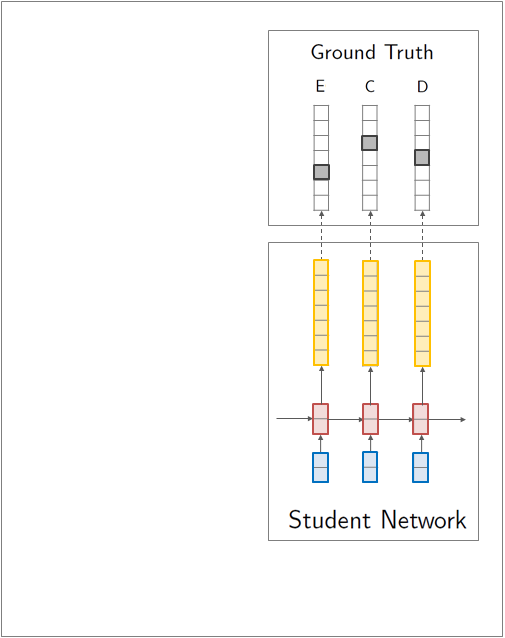
\includegraphics[trim={0.5cm 0.5cm 0.5cm 0.5cm}, clip, width=6cm]{word-kd-0}
% \end{column}
% \end{columns}
% \end{frame}

% \begin{frame}
% \centerline{\structure{Word-Level Knowledge Distillation}}
% \air
% \air
% \begin{columns}
% \begin{column}{6.5cm}
% Teacher network: $q(y_{t} | y_{1:t-1}, \cvec  ; \theta_T$)  \\
% \air
% \air
% Student network: $p(y_{t} | y_{1:t-1}, \cvec; \theta$)
% \end{column}
% \begin{column}{5.5cm}
% 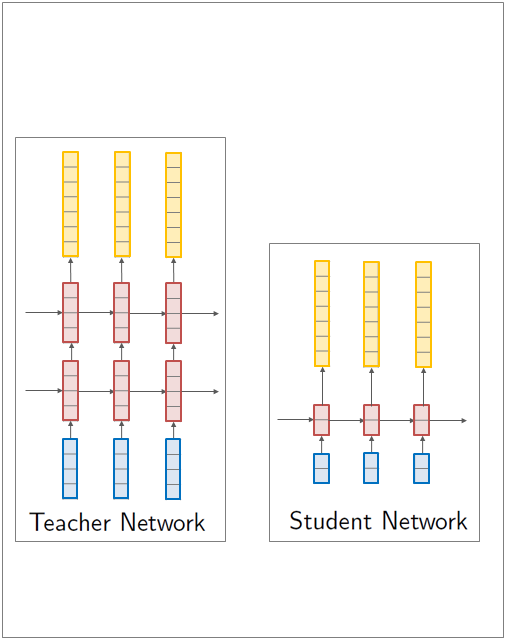
\includegraphics[width=5.5cm]{word-kd-1}
% \end{column}
% \end{columns}
% \end{frame}


\begin{frame}{Word-Level Knowledge Distillation (Multiclass)}

  \begin{center}
    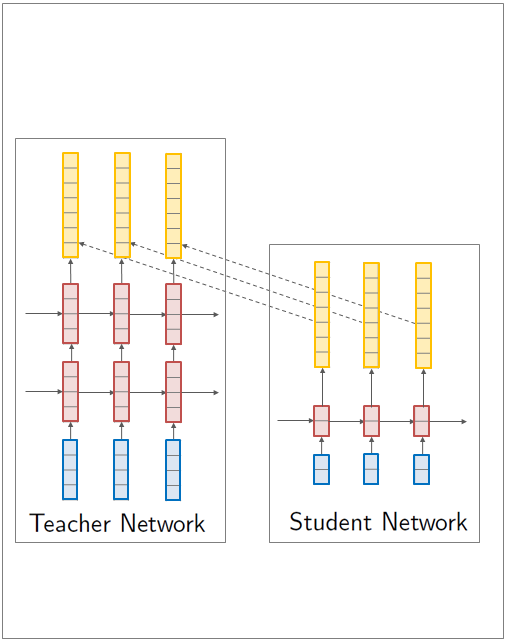
\includegraphics[trim={0.2cm 0.2cm 0.2cm 3cm}, clip,
    width=7cm]{word-kd-2}
  \end{center}
% \begin{columns}
% \begin{column}{7cm}
% Teacher model: $q(y_{t} | y_{1:t-1}, x; \theta_T$)
% \air

% Cross-entropy between teacher and student

% \begin{align*}
% \mathcal{L}_{\text{WORD-KD}}(\theta) = -\sum_t \sum_v &q(y_t=v \given \hat{y}_{1: t-1}, x ; \theta_T)\times \\
% & \log p(y_t =v \given \hat{y}_{1: t-1}, x ; \theta)
% \end{align*}
% \end{column}

% \begin{column}{7cm}
% \centering


% \end{column}
% \end{columns}
\end{frame}

% \begin{frame}
% \centerline{\structure{Word-Level Knowledge Distillation}}
% \air
% \begin{columns}
% \begin{column}{6.5cm}
% Add a term for NLL (equivalent to minimizing cross-entropy between student a mixture distribution of teacher/data distributions)
% \air
% $$\mathcal{L}(\theta) = \alpha\mathcal{L}_{\text{WORD-KD}}(\theta) + (1-\alpha)\mathcal{L}_{\text{NLL}}(\theta)$$
% \air
% $\alpha$ is a hyperparameter (we use $\alpha = 0.5$)
% \end{column}

% \begin{column}{5.5cm}
% 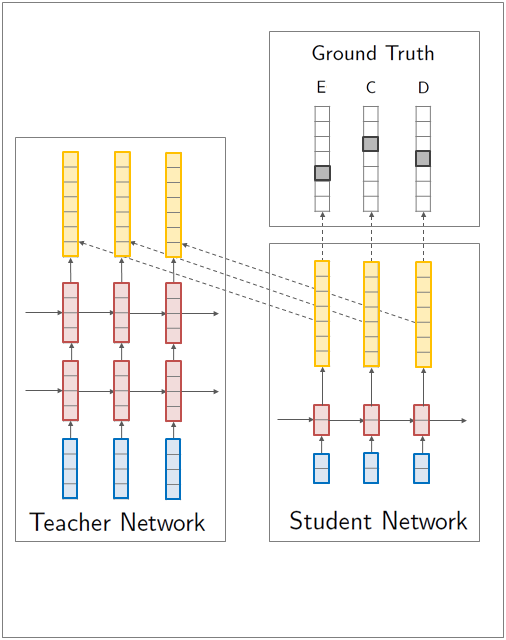
\includegraphics[width=5.5cm]{word-kd-3}
% \end{column}
% \end{columns}
% \end{frame}

% \begin{frame}{Sequence-Level Knowledge Distillation}
% \air
% \air

% \textbf{Motivation:} Replace multiclass with sequence-level cross-entropy.

% \begin{align*}
% \mathcal{L}_{\text{WORD-KD}}(\theta) = -\sum_t \sum_v &q(y_t=v \given \hat{y}_{1: t-1}, x ; \theta_T)\times  \log p(y_t =v \given \hat{y}_{1: t-1}, \cvec ; \theta)
% \end{align*}
% \[ \Downarrow \]
% \[ \mathcal{L}_{\text{SEQ-KD}}(\theta) = -\sum_{v_1} \ldots \sum_{v_T} q(y_{1:T}= v_{1:T}  | x; \theta_T) \times \log p(y_{1:T}=v_{1:T} | x ; \theta)
% \]

% Mimic sequence output of teacher model.
% \air

% Note: bottom distribution is again intractable.


% \end{frame}

% \begin{frame}{Sequence Heuristic Approximation}
% \air
% \air

% %\centerline{Sequence-Level Knowledge Distillation}
% \begin{columns}
% \begin{column}{6cm}
% Approximate $q(y_{1:T} \given x )$ with (beam search) mode sample
% $$q(y_{1:T} \given x ) \approx \mathbf{1}\{\argmax_{y} q(y_{1:T} \given x )\}$$
% % \air
% % $$ y^*_{1:T} \approx  \argmax_{y_{1:T}} q(y_{1:T} \given x ) $$
% % \\
% % Empirically, point estimate captures
% % significant mass

% \end{column}
% \begin{column}{8cm}
% 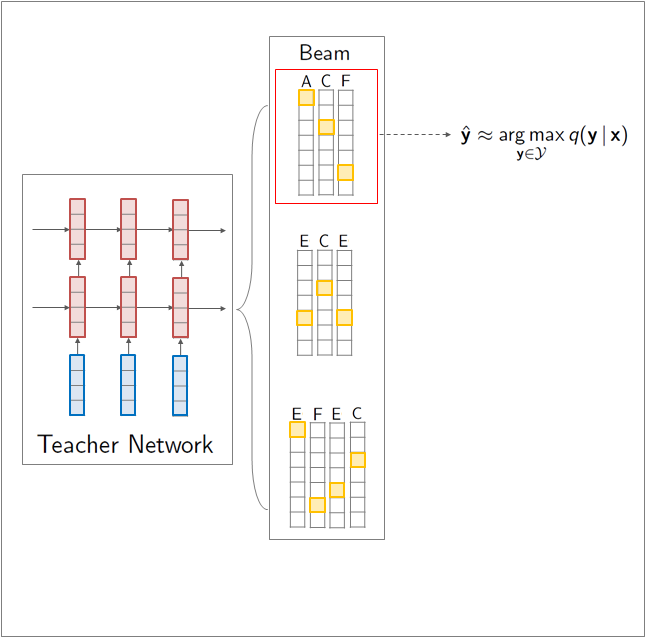
\includegraphics[trim={0.5cm 0.5cm 0.5cm 0.5cm}, clip, width=8cm]{seq-kd-1}
% \end{column}
% \end{columns}
% \end{frame}

\begin{frame}{Sequence-Level Knowledge Distillation}

% \begin{columns}
% \begin{column}{7cm}
% \begin{align*}
% \mathcal{L}_\text{SEQ-KD}(\theta) &= -\log p(y^*_{1:T} \given x ; \theta)  \\
% & \hspace*{-1cm} \displaystyle \approx   -\sum_{v_{1:T}} q(y_{1:T}=v_{1:t}|x; \theta_T) \log p(y_{1:T} | x ; \theta)
% \end{align*}
% \air

% Extension: $\mathcal{L}_\text{SEQ-INTER}(\theta)$ select sample based on ground truth $\hat{y}$
% as well.
% \end{column}
% \begin{column}{7cm}
  \begin{center}
    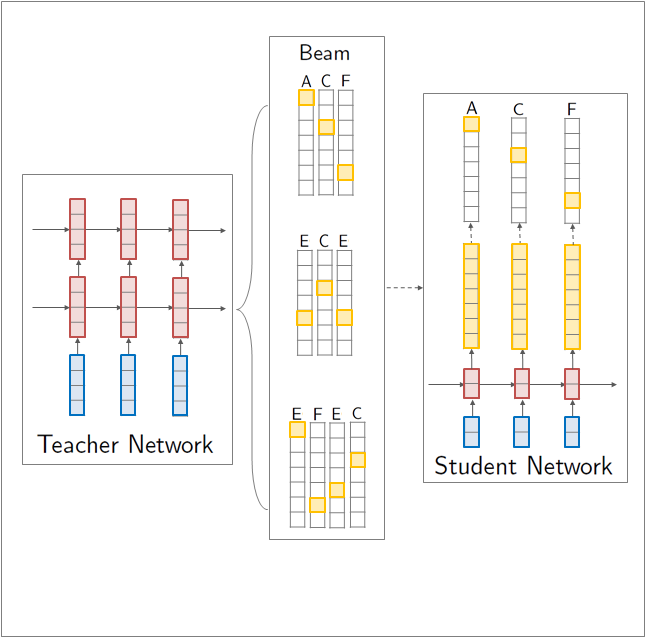
\includegraphics[trim={0.2cm 0.2cm 0.2cm 0.2cm}, clip,
    width=7cm]{seq-kd-2}
  \end{center}
% \end{column}
% \end{columns}
\end{frame}

\begin{frame}{Results: WMT English $\rightarrow$ German Translation}
\air
\air
\begin{table}
\centering
\begin{tabular}{lccccrr}
\toprule
Model &    BLEU$_{K=1}$   & $\Delta_{K=1}$ & BLEU$_{K=5}$ & $\Delta_{K=5}$ \\%& PPL & $p(y^*)$ \\
\midrule
$4 \times 1000$ \\
Teacher    & $17.7$ &  $-$ & $19.5$&   $-$ \\%&   $6.7$ &  $1.3\%$ \\
\midrule
\pause
$2 \times 500$ \\
\pause
Student  $\,$   & $14.7$ & $-$ & $17.6$&  $-$ \\%&  $8.2$ & $0.9\%$  \\
\hspace{1mm} Word-KD  & $15.4$ & $+0.7$& $17.7$& $+0.1$\\%&  $8.0$ & $1.0\%$  \\
\pause
% \hspace{1mm} Seq-KD   & $18.9$ & $+\mathbf{4.2}$& $19.0$& $+1.4$\\%&  $22.7$ & $                     \pause                                                         16.9\%$ \\
\hspace{1mm} Seq-KD  & $18.9$ & $+\mathbf{4.2}$&$19.3$ & $+\mathbf{1.7}$ \\ %&  $15.8$ & $7.6\%$  \\
% \midrule
% \pause
% $4 \times 1000$ \\
% \hspace{1mm} Seq-Inter    & $19.6$ & $+1.9$&  $19.8$& $+0.3$\\ %&   $10.4$ & $8.2\%$   \\
\bottomrule
\end{tabular}

\end{table}
\air
\air
\end{frame}

% \begin{frame}{Combining Knowledge Distillation and Pruning}
% \air
% \air
% \centering
% 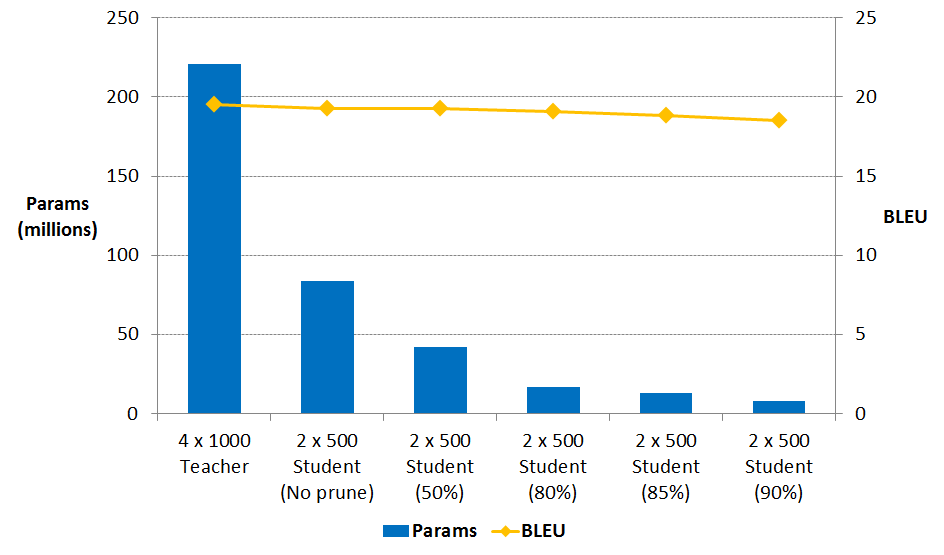
\includegraphics[width=0.8\textwidth]{modelsize}
% \end{frame}


\begin{frame}{Application}

  \begin{center}
    \movie[width=\textwidth, repeat, height=0.85\textheight, width=\textwidth, poster, showcontrols]{Temporary}{videos/translate.mp4}
  \end{center}
\end{frame}

% \begin{frame}{WNMT Translation Scaling Shared Task 2018}
%   (Results)
% \end{frame}

% 

\begin{frame}{ Outline}
  \begin{itemize}
  \item \textcolor{gray}{Background: Core Model and Implementation}
    \air
  \item \textcolor{gray}{Work 1: Rethinking Model Training}
    \air

  \item \textbf{Work 2: Rethinking  Generation  (\textit{Learning Neural Templates})}
    \air

  \item \textcolor{gray}{Challenges: Text Generation and Deep Learning}
  \end{itemize}

  \begin{center}
    \textbf{Can we learn interpretable and controllable target text generation models?}
  \end{center}

\end{frame}




% \begin{frame}{Part 4: Deep Latent-Variable Mdoels}

%    \begin{center}
%   \begin{tikzpicture}
%     \node[rounded corners, thick, draw] (ana) at (-15mm, 15mm) {Analysis};
%     \node[rounded corners, thick, fill=yellow,  draw] (meth) at (0mm, 30mm) {\ Methods\phantom{p}};
%     \node[rounded corners, thick, draw] (app) at (25mm, 30mm) {Applications};
%     \node[rounded corners, thick, fill=yellow, draw] (und) at (35mm, 15mm) {Understanding};
%     \node[rounded corners, thick, draw] (dep) at (25mm, 0mm){Scaling};
%     \node[rounded corners, thick, draw] (imp) at (0, 0) {Open-Source};
%     \draw (ana) -- (meth) --(app) -- (und) -- (dep) -- (imp) -- (ana);
%   \end{tikzpicture}
%   \end{center}
% \end{frame}


\begin{frame}{Talk about Data (E2EGen)}
  \vspace{-1cm}
  \begin{center}
    \begin{tikzpicture}

      \node (gal) {
\includegraphics[width=1.5cm]{phone}};
      \node [rounded corners, above =(0.2cm) of gal] {$f_\theta$};
      \node (a) [rectangle, yshift=1cm, xshift=-5cm, scale=0.7, draw,thick,fill=blue!0,text width=11em, rounded corners, inner sep =5pt, minimum height=1em] {
        \small
        \begin{tabular}[]{lc}
          \textbf{Fitzbillies} & \\
          \toprule
          type & coffee shop \\
          price & $<$ \pounds 20 \\
          food & Chinese \\
          rating  & 3/5 \\
          area & city centre \\
          \bottomrule
        \end{tabular}};



      % \path<2>[draw, ->] (a) --  (a -|  gal.west) ;


      \node [rounded corners, left =(0.2cm) of a] {\alert<1>{$x$}};
      \path[draw, ->] (a) --  (gal.west);
%       \visible<2->{
%         \node(b) [xshift=-5cm, yshift=-2.5cm, rectangle, scale=0.7, draw,thick,fill=blue!0,text width=18em, rounded corners, inner sep =5pt, minimum height=1em]{\baselineskip=50pt \small
% $\textcolor{gray}{|} $ $ \substack{\text{The \rule{15pt}{1pt}}\\\text{\rule{15pt}{1pt}}\\ \dots}
% \ \textcolor{gray}{|} \  $ $ \substack{\text{is a}\\\text{is an}\\\text{is an expensive}\\ \dots}
% \ \textcolor{gray}{|} \  $ $ \text{\rule{15pt}{1pt}} \ \textcolor{gray}{|} \  $ $ \substack{\text{providing}\\\text{serving}\\\text{offering}\\ \dots}
% \ \textcolor{gray}{|} \  $ $ \text{\rule{15pt}{1pt}} \ \textcolor{gray}{|} \  $ $ \substack{\text{food}\\\text{cuisine}\\\text{foods}\\ \dots}
% \ \textcolor{gray}{|} \  $ $ \text{in the} \ \textcolor{gray}{|} \  $ $ \substack{\text{high}\\\text{moderate}\\\text{less than average}\\ \dots}
% \ \textcolor{gray}{|} \  $ $ \substack{\text{price}\\\text{price range}\\ \dots}
% \ \textcolor{gray}{|} \  $ $ \text{.}$ $\textcolor{gray}{|}$ $ \text{It is} \ \textcolor{gray}{|} \  $ $ \substack{\text{located in the}\\\text{located near}\\\text{near}\\ \dots}
% \ \textcolor{gray}{|} \  $ $ \text{\rule{15pt}{1pt}} \ \textcolor{gray}{|} \  $ $ \text{.}$ $ \textcolor{gray}{|} \  $ $ \substack{\text{Its customer rating is}\\\text{Their customer rating is}\\\text{Customers have rated it}\\ \dots}
% \ \textcolor{gray}{|} \  $ $ \text{\rule{15pt}{1pt} out of \rule{15pt}{1pt}} \ \textcolor{gray}{|} \  .$
%           \par};

%         \node [rounded corners, above = (0.1cm) of b] {$z_{1:T}$};
%         \path[draw, ->] (b) --  (gal.west);
%       }

      \visible<2->{
        \node(c) [xshift=4.5cm, rectangle, scale=0.75, draw,thick,fill=blue!0,text width=20em, rounded corners, inner sep =5pt, minimum height=1em] {\baselineskip=50pt \small Fitzbillies   is a     coffee shop   providing   Chinese food  in the   moderate  price range .  It is   located in the city centre  .  Its customer rating is  3 out of 5 . \par };
      \node [rounded corners, above = (0.1cm) of c] { $y_{1:T}$};
      \path[draw, ->] (gal.east) -- (c);
    }


    \end{tikzpicture}
  \end{center}
\end{frame}


\begin{frame}{Talking About Data (WikiBio)}
  \begin{center}
    \mair
    \mair


    \begin{tikzpicture}

      \node (gal) {
\includegraphics[width=1.5cm]{phone}};
      \node [rounded corners, above =(0.2cm) of gal] {$f_\theta$};


      \node (a) [rectangle, yshift=2cm, xshift=-4.5cm, scale=0.8, draw,thick,fill=blue!0,text width=11.5em, rounded corners, inner sep =5pt, minimum height=1em] {\centering
        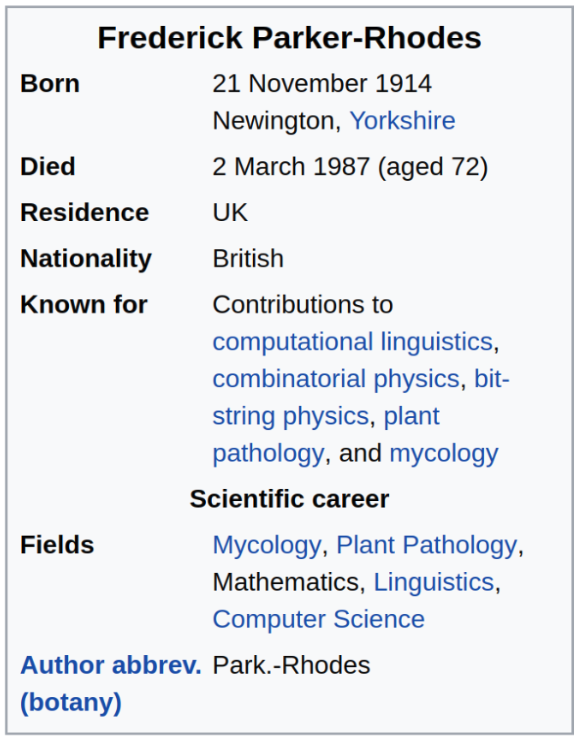
\includegraphics[width=4.5cm]{wiki}};
      \path[draw, ->] (a) --  (gal.west) ;


      \node [rounded corners, left =(0.2cm) of a] {{$x$}};

      \visible<4 - >{
        \node(b) [xshift=-4.5cm, yshift=-1.5cm, rectangle, scale=0.7, draw,thick,fill=blue!0,text width=12em, rounded corners, inner sep =5pt, minimum height=1em]{\baselineskip=50pt \small
 \rule{15pt}{1pt} (born \rule{15pt}{1pt}) was a
\rule{15pt}{1pt} \rule{15pt}{1pt} , who
lived in the \rule{15pt}{1pt} . He was
known for contributions to \rule{15pt}{1pt} .
          \par};

        \node [rounded corners, left = (0.1cm) of b] {$z_{1:T}$};
        \path[draw, ->] (b) --  (gal.west);
      }


      \visible<2>{
        \node(b) [xshift=4.5cm, yshift=-0cm, rectangle, scale=0.8, draw,thick,fill=blue!0,text width=12em, rounded corners, inner sep =5pt, minimum height=1em]{\baselineskip=50pt \small
          Frederick Parker-Rhodes
(21 November 1914 - 2
March 1987) was an
English linguist, plant
pathologist, computer
scientist, mathematician,
mystic, and mycologist.
          \par};

        \node [rounded corners, above = (0.2cm) of b] {$y_{1:T}$};
        \path[draw, <-] (b) --  (b -| gal.east) ;
      }

      \visible<3>{
        \node(b) [xshift=4.5cm, yshift=-0cm, rectangle, scale=0.8, draw,thick,fill=blue!0,text width=12em, rounded corners, inner sep =5pt, minimum height=1em]{\baselineskip=50pt \small
          Frederick Parker-Rhodes (21 November
1914 - 2 March 1987) was an English
mycology and \alert{plant pathology,
mathematics at the University of UK}.
          \par};

        \node [rounded corners, above = (0.2cm) of b] {$y^*_{1:T}$};
        \path[draw, <-] (b) --  (b -| gal.east) ;
      }

      \visible<5>{
        \node(b) [xshift=4.5cm, yshift=-0cm, rectangle, scale=0.8, draw,thick,fill=blue!0,text width=12em, rounded corners, inner sep =5pt, minimum height=1em]{\baselineskip=50pt \small
          \underline{Frederick Parker-Rhodes} (born \underline{21 November 1914}) was a \underline{English
mycologist} who
lived in the \underline{UK}. He was
known for contributions to \underline{plant pathology}.
          \par};

        \node [rounded corners, above = (0.2cm) of b] {$y^*_{1:T}$};
        \path[draw, <-] (b) --  (b -| gal.east) ;
      }



    \end{tikzpicture}
  \end{center}
\end{frame}


% \begin{frame}{Alternative Approach: Templated Generation}
%   \begin{center}
%     \begin{tikzpicture}

%       \node (gal) {
\includegraphics[width=1.5cm]{phone}};
%       \node [rounded corners, above =(0.2cm) of gal] {$\theta$};


%       \node (a) [rectangle, yshift=1cm, xshift=-5cm, scale=0.8, draw,thick,fill=blue!0,text width=13em, rounded corners, inner sep =5pt, minimum height=1em] {
%         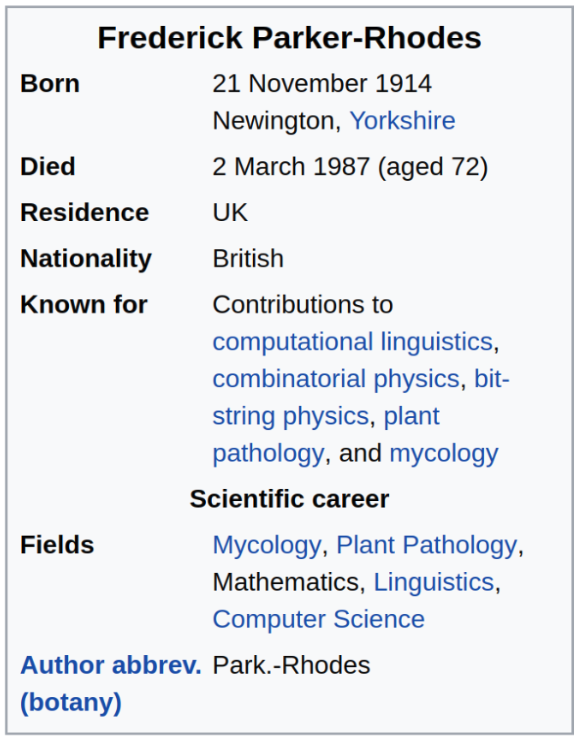
\includegraphics[width=5cm]{wiki}};
%       \path[draw, ->] (a) --  (a -|  gal.west) ;


%       \node [rounded corners, above =(0.2cm) of a] {{$x$}};

%       \visible{
%         \node(b) [xshift=4.5cm, yshift=-1cm, rectangle, scale=0.8, draw,thick,fill=blue!0,text width=12em, rounded corners, inner sep =5pt, minimum height=1em]{\baselineskip=50pt \small
%           [name] (born [born]) was a
% [nationality] [occupation], who
% lived in the [residence]. He was
% known for contributions to [known\_for].

%           \par};

%         \node [rounded corners, above = (0.2cm) of b] {$y_{1:T}$};
%         \path[draw, <-] (b) --  (b -| gal.east) ;
%       }




%     \end{tikzpicture}
%   \end{center}

% \end{frame}


\begin{frame}{Arguments for Templated Generation}
Guarantees about the quality, in particular,
\air


\begin{itemize}
\item \textbf{Interpretable} in its factual content.
  \air


  \air

\item \textbf{Controllable} in terms of style.
  \air


\end{itemize}

\begin{center}
  Can we achieve these criteria within a deep learning system?
\end{center}


\begin{enumerate}
\item Model
\item Training
\item Template Extraction
\end{enumerate}
\end{frame}


\begin{frame}{Technical Approach: Deep Latent-Variable Models}

  Expose specific choices as latent variables $z$.


\begin{align*}
p(y, z\ |\ x \param \theta)
\end{align*}

\begin{itemize}
    \item $x, y, \theta$ as before, \textit{what to talk about, how to say it}
    \item $z$ is a collection of problem-specific latent variables
\end{itemize}

% \begin{itemize}
%     \item Data consists of $N$ i.i.d samples,
% \end{itemize}

%                 \[ p(x^{(1:N)}, z^{(1:N)} \param \theta ) = \prod_{n=1}^N p(x^{(n)} \given z^{(n)}; \theta) p(z^{(n)};\theta). \]

\end{frame}

\begin{frame}{Example: Discrete Variables as Clusters}

Generative process:
\begin{enumerate}
\item Draw cluster $z \in \{1, \ldots, Z\}$ from a Categorical.
\item Draw words $y_{1:T}$ from decoder RNN with parameters $\pi_z$.
\end{enumerate}
\[p(y, z\ |\  x \param \theta)
       = \mu_{z} \times   \RNN(y_{1:T} \param \pi_z) \]
% \[p(x, z \param \theta)
%       = \mu_{z} \times  \prod_{t=1}^T \softmax(\RNN(\boldh_{t-1}, x_t\param \pi_z))\]
\begin{center}

\begin{tikzpicture}
  %\tikz{
% nodes
\node (dots) {$\ldots$};%
 \node[obs, left=1cm of dots] (x1) {$y_1$};%
 \node[obs, right=1cm of dots] (xT) {$y_T$};%
 \node[latent, above=of dots, fill=red!20] (z) {$z$}; %
 \node[const, above=(0.5cm) of z] (mu) {$\mu$};
 \node[const, below left=0.3cm and 0.8cm of x1] (pi) {$\pi$};

% plate
 % \plate {plate1} {(dots)(x1)(xT)(z)} {$N$}; %
% edges
 \edge {z} {dots};
 \edge {z} {x1};
 \edge {z} {xT};
 \edge {mu} {z};
 \edge {pi.east} {x1,xT.south};
 \edge {x1} {dots};
 %\edge[bend left] {x1.south} {xT.south};
  \edge {dots} {xT};

 \draw[->]
 (x1) edge[bend right=10] node [right] {} (xT);
 %}
 \node(a) [right=(3cm) of mu, fill=red!20]{The film is the first from ... };
 \node (aa) [right=(0.2cm) of a]{$z=1$};
 \node(b)[below = of a, fill=blue!20]{Allen shot four-for nine ... };
 \node (bb) [below= of aa]{$z=2$};
 \node(c) [below = of b, fill=orange!20]{In the last poll Ericson led ...};
 \node (cc) [below=of bb]{$z=3$};
 \end{tikzpicture}
 %}
\end{center}
%\begin{align*}
%\boldh_{z,t} &= \tanh(\mathbf{W}_z \bolde_t +\mathbf{U}_z\boldh_{z,t-1}  + \boldb_{z}) \nonumber \\
%p(x_{t} \given x_{<t} , z) &= \softmax(\mathbf{V} \boldh_{z,t-1} + \boldc)_{x_{t}} \nonumber \\
%p(x_1, \ldots, x_T \given z) &= \prod_{t=1}^{T} p(x_{t} \given x_{<t} , z)
%\end{align*}


\end{frame}


% begin{frame}
% \begin{center}
%     \textbf{ Latent-Variable Model Basics }
%   \end{center}


% \begin{align*}
% p(x, z \param \theta).
% \end{align*}

% \pause
% \begin{itemize}
%     \item $x$ is our observed data
%     \item $z$ is a collection of latent variables
%     \item $\theta$ are the deterministic parameters of the model, such as the neural network parameters
% \end{itemize}

% \pause

% \begin{itemize}
%     \item Data consists of $N$ i.i.d samples,
% \end{itemize}


%                 \[ p(x^{(1:N)}, z^{(1:N)} \param \theta ) = \prod_{n=1}^N p(x^{(n)} \given z^{(n)}; \theta) p(z^{(n)};\theta). \]
% \end{frame}

% \begin{frame}{Posterior Inference}
%     We'll be interested in the \textit{posterior} over latent variables $z$:

%     \begin{align*}
%         p(z \given y, x \param \theta) = \frac{\displaystyle p(y, z | x  \param \theta)}{\displaystyle p(y | x  \param \theta)} = \frac{\displaystyle p(y\given x, z \param  \theta) p(z | x  \param  \theta)}{\displaystyle \sum_{z'} p(y \given x, z'\param  \theta) p(z'| x\param  \theta) }.
%     \end{align*}

%     \air

%     \pause
%     % Why?
%     % \begin{itemize}
%     %   \item Required for training
%     %   \item Latent $z$ gives separation of data.

% % \item Intuition: if I know likely $z^{(n)}$ for $x^{(n)}$, I can learn by maximizing $p(x^{(n)} \given z^{(n)} \param \theta)$.
%         % \begin{itemize}
%         %     \item Intuition: if I know likely $z^{(n)}$ for $x^{(n)}$, I can learn by maximizing $p(x^{(n)} \given z^{(n)} \param \theta)$.
%         % \end{itemize}
%     % \end{itemize}

%     How?

%     \begin{itemize}
%     \item Sum out over all discrete choices (e.g. run $K$ RNNs).
%     \item Variational inference based methods.
%     \end{itemize}

% \end{frame}


% \begin{frame}{Preliminary Model 2: Copy Model}
% %{(Gu et al, 2016) (Gulcehre et al, 2016)}

% Generative process:
% \begin{enumerate}
% \item Draw copy switch $z_t \in \{0, 1\}$ from a Bernoulli.
% \item Draw words $y_t$ wherre
% \begin{itemize}
% \item If $z = 0$, generate a new word from the decoder.
%   \air
% \item If $z = 1$, copy a word from the source data.
% \end{itemize}

% \end{enumerate}

% \air
% \air

% Example:
% \begin{center}
% \underline{Frederick Parker-Rhodes} (born \underline{21 November
% 1914}) was a English \underline{linguist} $\ldots$


% % \centerline{\small (See et al, 2017)}
% \end{center}
% \end{frame}


\begin{frame}{Hidden Semi-Markov Model}

  \air
  \begin{itemize}

  \item Each discrete cluster produces multiple emissions (e.g. phrases).
    \air

  \item Parameterized with \textit{transition}
      and \textit{emission} distributions.
      \air

  \end{itemize}

  \begin{figure}
    \centering
    \begin{tikzpicture}[node distance=0.6cm]
    % \draw [step=0.2cm,gray,very thin] (-1.11, -1.11) grid  (1.1, 1.11);
    \node [circle](x){$$} ;
    \node[circle, draw, above right=of x, xshift = 1cm, fill=red!20](z){$z_1$};
    \node[ draw, rounded corners, below=of z, fill=red!10](rnn){};
    \node[circle, draw, below= of rnn](y){$y_1$};
    \node[circle, draw, right= of y](ya){$y_2$};
    \node[circle, draw, right= of ya](yb){$y_3$};
    \node[circle, draw, right= of yb](yc){$y_4$};
    \node[draw, rounded corners,  above= of yc, fill=blue!10](rnnb){};
    \node[circle, draw, above= of rnnb, fill=blue!20](zb){$z_{4}$};
    \draw[-] (z) -- (rnn) -- (y);
    \draw[-]  (rnn) -- (ya);
    \draw[-] (rnn) -- (yb);

    \draw[-] (zb) -- (rnnb) -- (yc);
     \draw (z) --node(mlp)[fill=white, draw, rounded corners]{} (zb);
     % \draw (x.north) edge [bend left=40] (mlp);
     % \draw (x) edge[] (rnn);
     % \draw (x) edge[bend left=20] (rnnb);

    \end{tikzpicture}
  \end{figure}

\end{frame}


\begin{frame}{Model: A Deep Hidden Semi-Markov Model}

  \begin{itemize}
  \item Employ HSMM as a conditional latent variable language model, $p(y_1, \ldots, y_T, z\ |\ x)$.

    \air
  \item Transition Distribution: neural network between clusters.

    \air
  \item Emission Distribution: Encoder-Decoder, specialized per cluster $\{1, \ldots, Z\}$.


  \end{itemize}

  \begin{figure}
    \centering
    \begin{tikzpicture}[node distance=0.6cm]
    \draw [step=0.2cm,gray,very thin] (-1.11, -1.11) grid  (1.1, 1.11);
    \node [draw, circle, fill=black!10](x){$x$} ;
    \node[circle, draw, above right=of x, xshift = 1cm, fill=red!20](z){$z_1$};
    \node[ draw, rounded corners, below=of z, fill=red!10](rnn){Decoder};
    \node[circle, draw, below= of rnn](y){$y_1$};
    \node[circle, draw, right= of y](ya){$y_2$};
    \node[circle, draw, right= of ya](yb){$y_3$};
    \node[circle, draw, right= of yb](yc){$y_4$};
    \node[draw, rounded corners,  above= of yc, fill=blue!10](rnnb){Decoder};
    \node[circle, draw, above= of rnnb, fill=blue!20](zb){$z_{4}$};
    \draw[-] (z) -- (rnn) -- (y);
    \draw[-]  (rnn) -- (ya);
    \draw[-] (rnn) -- (yb);

    \draw[-] (zb) -- (rnnb) -- (yc);
     \draw (z) --node(mlp)[fill=white, draw, rounded corners]{T} (zb);
     \draw (x.north) edge [bend left=40] (mlp);
     \draw (x) edge[] (rnn);
     \draw (x) edge[bend left=20] (rnnb);

    \end{tikzpicture}

    % \caption{HSMM factor graph (under a fixed segmentation) to illustrate parameters. Here we assume $z_1$ is in the ``red'' state (out of $K$ possibilities), and transitions to the ``blue'' state after emitting three words. The transition model, shown as $T$, is a function of the two states and the neural encoded source $x$. The emission model is a function of a ``red'' RNN model (with copy attention over $x$) that generates words 1, 2 and 3. After transitioning, the next word $y_4$ is generated by the ``blue'' RNN, but independently of the previous words.}
    \label{fig:my_label}
  \end{figure}
\end{frame}

\begin{frame}{Training}

  Training requires summing over clusters and segmentation of deep model.
    \[ {\cal L}(\theta) =  - \log \sum_{z_{1:T}} p(\hat{y}_{1:T}, z_{1:T} \ |\ x; \theta)\]
    \pause
    \centerline{\textbf{Example}}

    \begin{center}


Frederick Parker-Rhodes  was an English linguist, plant pathologist
    \begin{center}
      $\Downarrow \sum_{z_{1:T}}$
    \end{center}
\colorbox{green}{Frederick Parker-Rhodes}  \colorbox{red}{was an English} \colorbox{skyblue}{linguist}, \colorbox{redpurple}{plant pathologist} $\ldots$\\ \pause
\colorbox{red}{Frederick} \colorbox{redpurple}{Parker-Rhodes}  \colorbox{red}{was an\phantom{D}} \colorbox{skyblue}{English linguist}, \colorbox{green}{plant pathologist} $\ldots$\\ \pause
\colorbox{redpurple}{Frederick}  \colorbox{orange}{Parker-Rhodes was an English linguist ,} \colorbox{skyblue}{linguist}, \colorbox{redpurple}{plant pathologist} $\ldots$
    \end{center}
\end{frame}

% \begin{frame}{Technical Methodology}
%     \begin{itemize}
%     \item Requires summing over all clusters and segmentation.
%     \item Approach: backprop through HSMM dynamic programming algorithm, exact gradient.
%     \item Gives a new definition for $f_\theta(y_{1:T}, x)$
%     \end{itemize}
% \end{frame}


\begin{frame}{Template Extraction}
  Extract templates by finding most common, best latent sequences from training.
  \begin{figure}
    \centering
    \scalebox{0.5}{
    \begin{tikzpicture}[node distance=0.6cm]
    \draw [step=0.2cm,gray,very thin] (-1.11, -1.11) grid  (1.1, 1.11);
    \node [draw, circle, fill=black!10](x){$x$} ;
    \node[circle, draw, above right=of x, xshift = 1cm, fill=red!20](z){$z_1$};
    \node[ draw, rounded corners, below=of z, fill=red!10](rnn){Decoder};
    \node[circle, draw, below= of rnn](y){$y_1$};
    \node[circle, draw, right= of y](ya){$y_2$};
    \node[circle, draw, right= of ya](yb){$y_3$};
    \node[circle, draw, right= of yb](yc){$y_4$};
    \node[draw, rounded corners,  above= of yc, fill=blue!10](rnnb){Decoder};
    \node[circle, draw, above= of rnnb, fill=blue!20](zb){$z_{4}$};
    \draw[-] (z) -- (rnn) -- (y);
    \draw[-]  (rnn) -- (ya);
    \draw[-] (rnn) -- (yb);

    \draw[-] (zb) -- (rnnb) -- (yc);
     \draw (z) --node(mlp)[fill=white, draw, rounded corners]{T} (zb);
     \draw (x.north) edge [bend left=40] (mlp);
     \draw (x) edge[] (rnn);
     \draw (x) edge[bend left=20] (rnnb);
    \end{tikzpicture}
}
    % \caption{HSMM factor graph (under a fixed segmentation) to illustrate parameters. Here we assume $z_1$ is in the ``red'' state (out of $K$ possibilities), and transitions to the ``blue'' state after emitting three words. The transition model, shown as $T$, is a function of the two states and the neural encoded source $x$. The emission model is a function of a ``red'' RNN model (with copy attention over $x$) that generates words 1, 2 and 3. After transitioning, the next word $y_4$ is generated by the ``blue'' RNN, but independently of the previous words.}
  \end{figure}
    \[ z_{1:T}^* = \argmax_{z_{1:T}} p(y_{1:T}, z_{1:T} \ |\ x; \theta)\]
    \pause
    \centerline{\textbf{Example}}
    \begin{center}


Frederick Parker-Rhodes  was an English linguist, plant pathologist
    \begin{center}
      $\Downarrow \argmax_{z_{1:T}}$
    \end{center}
\colorbox{green}{Frederick Parker-Rhodes}  \colorbox{red}{was an English} \colorbox{skyblue}{linguist}, \colorbox{redpurple}{plant pathologist} $\ldots$\\ \pause
    \end{center}
\end{frame}

\begin{frame}{Template Grouping}
  Find templates $z_{1:T}$ that occur most often in the data.
\air
\begin{center}


Frederick Parker-Rhodes  was an English linguist, plant pathologist
    \begin{center}
      $\Downarrow \argmax_{z_{1:T}}$
    \end{center}
\colorbox{green}{Frederick Parker-Rhodes}  \colorbox{red}{was an English} \colorbox{skyblue}{linguist}, \colorbox{redpurple}{plant pathologist} $\ldots$\\ \pause
\air
\air

Bill Jones  was an American professor, and well-known author
    \begin{center}
      $\Downarrow \argmax_{z_{1:T}}$
    \end{center}

\colorbox{green}{Bill Jones}  \colorbox{red}{was an American} \colorbox{skyblue}{professor}, \colorbox{redpurple}{and well-known author} $\ldots$\\ \pause
\end{center}

\end{frame}




\begin{frame}{Example Templates: Wikipedia}

  Extracted templates $z_{1:T}^*$ and their generated words.

  \begin{center}
    \includegraphics[trim={5cm 5cm 0.2cm 0cm}, clip, width=0.9\textwidth]{extemp}
  \end{center}
\end{frame}



\begin{frame}{Technical Methodology}

  Training is end-to-end, i.e. clusters and segmentation are learned
  simultaneously with encoder-decoder model on GPU.


  \begin{itemize}
  \item  Training Technique: Backpropagation through dynamic programming. Parameters are trained by exactly marginalizing over segmentations (HSMM backward algorithms)
  \end{itemize}
  \air

  \begin{itemize}
  \item Extraction Technique: Viterbi algorithm over encoder-decoder potentials.
  \end{itemize}


\end{frame}






% \begin{frame}{ Latent Variable Models for Generation}
%   \textbf{Ongoing Work:} Can we develop other discrete latent-variable models for generation?

%   \air

%   \textbf{Goals:}

%     \begin{itemize}
%     \item Model Control
%     \item Model Debugging
%     \item Model Uncertainty
%     \end{itemize}
% \end{frame}




% \begin{frame}
%   \begin{figure}
%     \centering

%     \footnotesize
% \begin{tabular}{@{}ll@{}}
% \toprule
% \bf Meaning Representation        & \begin{tabular}[c]{@{}l@{}}name{[}The Golden Palace{]},  eatType{[}coffee shop{]},  food{[}Fast food{]}, \\ priceRange{[}cheap{]},  customer rating{[}5 out of 5{]},  area{[}riverside{]}\end{tabular}         \\ \midrule
% \bf Reference & \begin{tabular}[c]{@{}l@{}}A coffee shop located on the riverside  called The Golden Palace,  \\ has a 5 out of 5 customer rating.  Its price range are fairly cheap  \\for its excellent Fast food.\end{tabular} \\ \bottomrule
% \end{tabular}
%   \end{figure}

% \end{frame}

% \begin{frame}{Standard Approach}


% \textbf{Step 1: Encode the Source}
% \air

% \begin{small}
% Fitzbillies,type[coffee shop],price[$<$ \pounds 20],food[Chinese],rate[3/5],area[city centre]
% \end{small}

% \vspace{0.3cm}

% \textbf{Step 2: Generate with RNN Decoder}

% \air

% \underline{Fitzbillies}  is a  \underline{coffee shop}  providing  \underline{Chinese} food in the  moderate  price range  .  It is  located in the  \underline{city centre}  .  Its customer rating is  \underline{3} out of \underline{5}.

% \end{frame}

% \begin{frame}{Issues}
% \begin{enumerate}
% \item Interpretable in its content selection?
%   \air

%   \textit{Decisions may come from anywhere in the source $x$.}

%   \air

% \item Controllable in terms of style and form?
%   \air

%   \textit{Rely on a learned system to determine content.}
% \end{enumerate}

%\end{frame}

\begin{frame}{Neural Template Generation Approach}
  \vspace{-1cm}
  \begin{center}
    \begin{tikzpicture}

      \node (gal) {\includegraphics[width=1.5cm]{phone}};
      \node [rounded corners, above =(0.2cm) of gal] {$f_\theta$};
      \node (a) [rectangle, yshift=1cm, xshift=-5cm, scale=0.7, draw,thick,fill=blue!0,text width=11em, rounded corners, inner sep =5pt, minimum height=1em] {
        \small
        \begin{tabular}[]{lc}
          \textbf{Fitzbillies} & \\
          \toprule
          type & [coffee shop] \\
          price & $<$ \pounds 20 \\
          food & Chinese \\
          rating  & 3/5 \\
          area & city centre] \\
          \bottomrule
        \end{tabular}};



      % \path<2>[draw, ->] (a) --  (a -|  gal.west) ;


      \node [rounded corners, above =(0.2cm) of a] {\alert<1>{$x$}};
      \path[draw, ->] (a) --  (gal.west);
      \visible<2->{
        \node(b) [xshift=-5cm, yshift=-2.5cm, rectangle, scale=0.7, draw,thick,fill=blue!0,text width=18em, rounded corners, inner sep =5pt, minimum height=1em]{\baselineskip=50pt \small
$\textcolor{gray}{|} $ $ \substack{\text{The \rule{15pt}{1pt}}\\\text{\rule{15pt}{1pt}}\\ \dots}
\ \textcolor{gray}{|} \  $ $ \substack{\text{is a}\\\text{is an}\\\text{is an expensive}\\ \dots}
\ \textcolor{gray}{|} \  $ $ \text{\rule{15pt}{1pt}} \ \textcolor{gray}{|} \  $ $ \substack{\text{providing}\\\text{serving}\\\text{offering}\\ \dots}
\ \textcolor{gray}{|} \  $ $ \text{\rule{15pt}{1pt}} \ \textcolor{gray}{|} \  $ $ \substack{\text{food}\\\text{cuisine}\\\text{foods}\\ \dots}
\ \textcolor{gray}{|} \  $ $ \text{in the} \ \textcolor{gray}{|} \  $ $ \substack{\text{high}\\\text{moderate}\\\text{less than average}\\ \dots}
\ \textcolor{gray}{|} \  $ $ \substack{\text{price}\\\text{price range}\\ \dots}
\ \textcolor{gray}{|} \  $ $ \text{.}$ $\textcolor{gray}{|}$ $ \text{It is} \ \textcolor{gray}{|} \  $ $ \substack{\text{located in the}\\\text{located near}\\\text{near}\\ \dots}
\ \textcolor{gray}{|} \  $ $ \text{\rule{15pt}{1pt}} \ \textcolor{gray}{|} \  $ $ \text{.}$ $ \textcolor{gray}{|} \  $ $ \substack{\text{Its customer rating is}\\\text{Their customer rating is}\\\text{Customers have rated it}\\ \dots}
\ \textcolor{gray}{|} \  $ $ \text{\rule{15pt}{1pt} out of \rule{15pt}{1pt}} \ \textcolor{gray}{|} \  .$
          \par};

        \node [rounded corners, above = (0.1cm) of b] {$z_{1:T}$};
        \path[draw, ->] (b) --  (gal.west);
      }

      \visible<3->{
        \node(c) [xshift=4.5cm, rectangle, scale=0.75, draw,thick,fill=blue!0,text width=20em, rounded corners, inner sep =5pt, minimum height=1em] {\baselineskip=50pt \small $\|$  Fitzbillies $\|$   is a $\|$    coffee shop $\|$   providing $\|$  Chinese $\|$ food $\|$ in the $\|$  moderate $\|$ price range $\|$ . $\|$ It is  $\|$ located in the $\|$ city centre $\|$ . $\|$ Its customer rating is $\|$ 3 out of 5 $\|$ . \par };
      \node [rounded corners, above = (0.1cm) of c] { $y_{1:T}$};
      \path[draw, ->] (gal.east) -- (c);
    }


    \end{tikzpicture}
  \end{center}
\end{frame}

% \textbf{Step 1: Encode the Source}

% \begin{small}
% Fitzbillies,ty[coffee shop],pr[$<$ \pounds 20],food[Chinese],cust[3/5],area[city centre]
% \end{small}

% \pause
% \air
% \textbf{Step 2: Select a \textit{Template}}

%     \begin{center}

% $\textcolor{gray}{|} $ $ \substack{\text{The \rule{15pt}{1pt}}\\\text{\rule{15pt}{1pt}}\\ \dots}
% \ \textcolor{gray}{|} \  $ $ \substack{\text{is a}\\\text{is an}\\\text{is an expensive}\\ \dots}
% \ \textcolor{gray}{|} \  $ $ \text{\rule{15pt}{1pt}} \ \textcolor{gray}{|} \  $ $ \substack{\text{providing}\\\text{serving}\\\text{offering}\\ \dots}
% \ \textcolor{gray}{|} \  $ $ \text{\rule{15pt}{1pt}} \ \textcolor{gray}{|} \  $ $ \substack{\text{food}\\\text{cuisine}\\\text{foods}\\ \dots}
% \ \textcolor{gray}{|} \  $ $ \text{in the} \ \textcolor{gray}{|} \  $ $ \substack{\text{high}\\\text{moderate}\\\text{less than average}\\ \dots}
% \ \textcolor{gray}{|} \  $ $ \substack{\text{price}\\\text{price range}\\ \dots}
% \ \textcolor{gray}{|} \  $ $ \text{.}$ $\textcolor{gray}{|}$ $ \text{It is} \ \textcolor{gray}{|} \  $ $ \substack{\text{located in the}\\\text{located near}\\\text{near}\\ \dots}
% \ \textcolor{gray}{|} \  $ $ \text{\rule{15pt}{1pt}} \ \textcolor{gray}{|} \  $ $ \text{.}$ $ \textcolor{gray}{|} \  $ $ \substack{\text{Its customer rating is}\\\text{Their customer rating is}\\\text{Customers have rated it}\\ \dots}
% \ \textcolor{gray}{|} \  $ $ \text{\rule{15pt}{1pt} out of \rule{15pt}{1pt}} \ \textcolor{gray}{|} \  .$
%     \end{center}
% \pause
% \air
% \textbf{Step 3: Fill-in Each Segment}
%     \air


% $\|$ \underline{Fitzbillies} $\|$  \pause is a $\|$ \pause   \underline{coffee shop} $\|$ \pause  providing $\|$  \underline{Chinese} $\|$ food $\|$ in the $\|$  moderate $\|$ price range $\|$ . $\|$ It is  $\|$ located in the $\|$ \underline{city centre} $\|$ . $\|$


    % \caption{An example from the E2E Generation dataset~\citep{novikova2017e2e}; knowledge base $x$ (top) contains 5 records, and $\hat{y}$ (middle) is a system generation; records are shown as \texttt{type[value]}.
    % (bottom) An induced neural template learned by the system and employed in generating $\hat{y}$. %Each cell shows the possible output choices and each underscore represents a slot fillable with copy attention.
    % Each cell represents a segment in the learned segmentation, and underscores show where slots are (typically) filled through copy attention during generation.
    % }

% \end{frame}


% \begin{frame}{Criteria}

% \begin{enumerate}
% \item Interpretable in its content selection.
%   \air

%   \textit{Decisions are localized to a segment of the template.}

%   \air

% \item Easily controllable in terms of style and form.
%   \air

%   \textit{Alternative realizations through different templates.}
% \end{enumerate}


% \air

% \pause



% \alert{However:} templates feel much less ``end-to-end''.
% How can we learn them from data?

% \end{frame}



% \begin{frame}{Neural Template}
% \air

%       \begin{center}

% $\textcolor{gray}{|} $ $ \substack{\text{The \rule{15pt}{1pt}}\\\text{\rule{15pt}{1pt}}\\ \dots}
% \ \textcolor{gray}{|} \  $ $ \substack{\text{is a}\\\text{is an}\\\text{is an expensive}\\ \dots}
% \ \textcolor{gray}{|} \  $ $ \text{\rule{15pt}{1pt}} \ \textcolor{gray}{|} \  $ $ \substack{\text{providing}\\\text{serving}\\\text{offering}\\ \dots}
% \ \textcolor{gray}{|} \  $ $ \text{\rule{15pt}{1pt}} \ \textcolor{gray}{|} \  $ $ \substack{\text{food}\\\text{cuisine}\\\text{foods}\\ \dots}
% \ \textcolor{gray}{|} \  $ $ \text{in the} \ \textcolor{gray}{|} \  $ $ \substack{\text{high}\\\text{moderate}\\\text{less than average}\\ \dots}
% \ \textcolor{gray}{|} \  $ $ \substack{\text{price}\\\text{price range}\\ \dots}
% \ \textcolor{gray}{|} \  $ $ \text{.}$ $\textcolor{gray}{|}$ $ \text{It is} \ \textcolor{gray}{|} \  $ $ \substack{\text{located in the}\\\text{located near}\\\text{near}\\ \dots}
% \ \textcolor{gray}{|} \  $ $ \text{\rule{15pt}{1pt}} \ \textcolor{gray}{|} \  $ $ \text{.}$ $ \textcolor{gray}{|} \  $ $ \substack{\text{Its customer rating is}\\\text{Their customer rating is}\\\text{Customers have rated it}\\ \dots}
% \ \textcolor{gray}{|} \  $ $ \text{\rule{15pt}{1pt} out of \rule{15pt}{1pt}} \ \textcolor{gray}{|} \  .$
%     \end{center}
% \end{frame}

% \begin{frame}{Experimental Setup}

%   \begin{itemize}
%   \item Two datasets, E2E challenge and WikiBio
%     \air
%   \item Training with 35 and 65 state models, each 1x300 LSTMs.
%     \air
%   \item Extract 100 most common templates for each.
%     \air
%   \item Vocabulary limited to non-copy-able words.
%     \air

%   \item Generation with beam search with a pre-selected template.
%   \end{itemize}
% \end{frame}




% \begin{frame}{WikiBio (500k)}

%   \begin{center}



%       \begin{figure}[t]
% \centering
% \begin{tabular}{@{}l@{}}
% \toprule
% \\
% % \begin{tabular}[c]{c}
% %   \hspace{2.5cm}
% %     % \includegraphics[scale=0.7]{wbpage_cropped.pdf}
% % \end{tabular}
% \midrule
% \begin{tabular}[c]{@{}l@{}}
% {\small Frederick Parker-Rhodes (21 March 1914 - 21 November} \\
% {\small 1987) was an English linguist, plant pathologist, computer} \\
% {\small scientist, mathematician, mystic, and mycologist.}
% \end{tabular} \\
% \bottomrule
% \end{tabular}
% % \caption{An example from the WikiBio dataset~\citep{lebret2016neural} for entity \texttt{Frederick Parker-Rhodes}; $x$ (top) and $y$ (bottom) is the corresponding reference generation.}
% \label{fig:wbex}
% \end{figure}

%   \end{center}
% \end{frame}






% \begin{frame}{WikiBio}
% \begin{table}[t!]
% \small
% \centering
% \begin{tabular}{@{}lccc@{}}
% \toprule
%  & BLEU & NIST & ROUGE-4\\
% \midrule
% Conditional KN-LM  & 19.8 & 5.19 & 10.7 \\
% NNLM (field)  & 33.4 & 7.52 & 23.9 \\
% NNLM (field \& word)  & 34.7 & 7.98 & 25.8 \\
% Neural Template &  33.8 & 7.51 & 28.2 \\
% \bottomrule
% \end{tabular}
% \label{tab:wb}
% \end{table}

% \begin{itemize}
% \item Custom KN and NNLM Baselines from LeBret et al (2016)
% \end{itemize}k

% \end{frame}



% \begin{frame}
% \end{frame}


\begin{frame}{Arguments for Templated Generation}
Guarantees about the quality, in particular,
\air


\begin{itemize}
\item \textbf{Interpretable} in its factual content.
  \air


  \air

\item \textbf{Controllable} in terms of style.
  \air


\end{itemize}

\end{frame}



\begin{frame}[fragile]{Issue 1: Interpretable}

  \begin{center}



  \begin{table}[t]
\small
\centering

\begin{tabular}{@{}l@{}}
  \toprule
  \textbf{kenny warren} \\
  \midrule
  \begin{tabular}[c]{@{}l@{}}
    \textbf{name:} kenny warren, \textbf{birth date:} 1 april 1946, \\
    \textbf{birth name:} kenneth warren deutscher, \textbf{birth place:} brooklyn, new york, \\ \textbf{occupation:} ventriloquist, comedian, author, \\
    \textbf{notable work:} book - the revival of ventriloquism in america \\
  \end{tabular}         \\
  \midrule

  \begin{tabular}[c]{@{}l@{}}
    1. \colorbox{green}{kenny warren deutscher} (\colorbox{pink}{april 1, 1946}) is an \colorbox{cyan}{american} ventriloquist. \\
    2. \colorbox{green}{kenny warren deutscher} (\colorbox{pink}{april 1, 1946}, brooklyn,) is an \colorbox{cyan}{american} ventriloquist.\\
    3. \colorbox{green}{kenny warren deutscher} (\colorbox{pink}{april 1, 1946}) is an \colorbox{cyan}{american} \\
    \hspace{1cm} ventriloquist, best known for his the revival of ventriloquism. \\
    4. \colorbox{yellow}{``kenny'' warren} is an \colorbox{cyan}{american} ventriloquist. \\
5. kenneth warren \colorbox{yellow}{``kenny'' warren} (born \colorbox{pink}{april 1, 1946}) is  an \colorbox{cyan}{american} ventriloquist, and author. \\
\end{tabular} \\
\bottomrule
\end{tabular}
\label{tab:wbcontrol}
\end{table}

  \end{center}
\end{frame}


\begin{frame}{Controllable}

  \begin{table}[t]
\small
\centering
\begin{tabular}{@{}l@{}}
\toprule
\textbf{The Golden Palace} \\
\midrule
\begin{tabular}[c]{@{}l@{}}
name[The Golden Palace], type[coffee shop], food[Chinese], \\
priceRange[cheap] custRating[5 out of 5], area[city centre], \\
\end{tabular}         \\
\midrule
\begin{tabular}[c]{@{}l@{}}
1. The Golden Palace is a coffee shop located in the city centre. \\
2. In the city centre is a cheap Chinese coffee shop called  The Golden Palace. \\
3. The Golden Palace is a Chinese coffee shop. \\
4. The Golden Palace is a Chinese coffee shop  with a customer rating of 5 out of 5. \\
5. The Golden Palace that serves Chinese food in the cheap \\
\; \; price range. It is located in the city centre.  Its customer rating is 5 out of 5. \\

\end{tabular} \\
\bottomrule
\end{tabular}
% \caption{Impact of varying the template $z^{(i)}$ for a single $x$ from the E2E dataset.}
\label{tab:e2econtrol}
\end{table}
\end{frame}


\begin{frame}{Results}
\begin{table}[t!]
\small
\centering
\textbf{E2E}

\air

\includegraphics[width=10cm]{crop1}
\air

\textbf{WikiBio}
\air

\includegraphics[width=8cm]{crop2}
% \caption{Comparison of the system of \citet{duvsek2016sequence}, which forms the baseline for the E2E challenge, a non-parametric, substitution-based baseline (see text), and our HSMM model on the validation and test portions of the E2E dataset. ``ROUGE'' is ROUGE-L. Models are evaluated using the official E2E NLG Challenge scoring scripts.}
\label{tab:e2e}
\end{table}
\end{frame}



\begin{frame}{Outline}

  \begin{itemize}
  \item Background: Core Model and Implementation
    \air
  \item Work 1: Rethinking Model Training (\textit{Beam Search Optimization})
    \air

  \item Work 2: Rethinking  Generation  (\textit{Learning Neural Templates})
    \air
  \item \textbf{Challenges: Text Generation and Deep Learning}
  \end{itemize}
\end{frame}


% \begin{frame}{Three Challenge in Text Generation}
%   \begin{enumerate}
%   \item Long-Form Generation with High-Level Reasoning
%     \air
%   \item Compact and Efficient Generation
%     \air
%   \item Latent-Variable Modeling for NLP
%   \end{enumerate}
% \end{frame}

% \begin{frame}{Future Work}

%   \begin{center}
%   \begin{tikzpicture}
%     \node[rounded corners, draw] (ana) at (-15mm, 15mm) {Analysis};
%     \node[rounded corners, draw] (meth) at (0mm, 30mm) {\ Methods\phantom{p}};
%     \node[rounded corners, draw] (app) at (25mm, 30mm) {Applications};
%     \node[rounded corners, draw] (und) at (35mm, 15mm) {Understanding};
%     \node[rounded corners, draw] (dep) at (25mm, 0mm){Deployment};
%     \node[rounded corners, draw] (imp) at (0, 0) {Implement};
%     \draw (ana) -- (meth) --(app) -- (und) -- (dep) -- (imp) -- (ana);
%   \end{tikzpicture}
%   \end{center}
% \end{frame}

\begin{frame}{1) Long-Form Generation with Explicit Reasoning}
  \begin{center}
    \includegraphics[width=0.85\linewidth]{basketball}
  \end{center}
  % \begin{enumerate}
  % \item Discourse-aware structure in generation
  % \item Explicit Linking and coreference
  % \item Aggregation of factual information before generation
  % \end{enumerate}
\end{frame}

\begin{frame}{2) Controllable Interactive ML Systems}
  \research{w/ IBM}
  \begin{center}
    \includegraphics[width=0.7\textwidth]{DecoderVis}
  \end{center}
\end{frame}


\begin{frame}{2) Controllable Interactive ML Systems}

  \research{w/ IBM}
  \begin{center}
    \includegraphics[width=0.8\textwidth]{AttentionVIS}
  \end{center}
\end{frame}

\begin{frame}{3) Prob. Programming \& Deep Learning}
\research{w/ Uber}

\begin{center}
\includegraphics[width=3cm]{pyro} \hspace{2cm} \includegraphics[width=5cm]{pyro2}

\air
  \begin{tikzpicture}
\node[latent] (Y) {$y$};
\node[factor, xshift=1.25cm] (FYS) {$F$};
\node[latent, xshift=2.5cm](S) {$z$};
\node[factor, xshift=3.75cm](FS) {$G$};
\node[xshift=1.25cm, yshift=-0.5cm]() {$T$};
\node[obs, xshift=5cm](X) {$\mathbf{x}$};
\node[obs, xshift=2.5cm, yshift=1.3cm] (A) {$a$};
\node[obs, xshift=2.5cm, yshift=-1.45cm] (L) {$l$};


\plate [inner sep=0.1cm, xshift=0cm, yshift=0.0cm] {t} {(FS)(S)(FYS)} {};
\plate [inner xsep= 0.3cm, inner ysep= 0.2cm, xshift=-0.1cm, yshift=-0.1cm] {a} {(Y)(FYS)(S)(A)(FS)} {};
\plate [inner xsep= 0.3cm, inner ysep= 0.1cm, xshift=0.1cm, yshift=0.2cm] {l} {(Y)(FYS)(S)(L)(FS)} {};
\node[caption, below left=-0.1cm and -0.3cm of a-wrap.north west] {$|\cal{A}|$};
\node[caption, below left=-0.5cm and -0.4cm of l-wrap.south east] {$|\cal{L}|$};

\draw (Y) -- (FYS);
\draw (X) -- (FS);
\draw[-] (X) to [bend left=25] (FYS);
\draw (FYS) -- (S);
\draw (S) -- (FS);
\draw (FS) -- (A);
\draw (FS) -- (L);
\draw[-] (FYS) to [] (A);
\draw[-] (FYS) to [] (L);
\end{tikzpicture}

\end{center}
\end{frame}

\begin{frame}{4) Hardware Co-Design}
\research{w/ ARM}
\begin{center}
  \includegraphics[height=0.6\textheight]{testchip}
\end{center}
\end{frame}



% \begin{frame}{Learning Neural Reasoning-Based Models}
%   \begin{center}
%     \movie[width=\textwidth, repeat, height=0.85\textheight, width=\textwidth, poster, showcontrols]{Temporary}{videos/latnm.mp4}
%   \end{center}
% \end{frame}


\begin{frame}{Harvard NLP}
  \begin{center}
  \includegraphics[width=6cm]{Members}

  \includegraphics[width=2cm]{Members2}
  \end{center}
\end{frame}



\begin{frame}
  \url{http://lstm.seas.harvard.edu/client/lstmvis.html?project=00parens&source=states::states2&activation=0.3&cw=30&meta=..&pos=165}
  \url{http://lstm.seas.harvard.edu/client/lstmvis.html?project=05childbook&source=states::states1&activation=0.3&cw=30&meta=..&pos=100&wordBrush=..20,23&wordBrushZero=..1,0&sc=..55,59,159,167,174,179}

\end{frame}



\bibliography{me}
\bibliographystyle{acl_natbib_nourl}

\end{document}